\documentclass[twoside]{book}
\usepackage{problems}
\usepackage[colorlinks=true,
citecolor=black,
linkcolor=black,
anchorcolor=black,
filecolor=black,
menucolor=black,
urlcolor=black,
pdftitle={Puzzles in geometry which I know and love},
pdfsubject={Geometry},
pdfauthor={Anton Petrunin}
]{hyperref}
\makeindex

\begin{document}


\title{Puzzles in geometry \\
which I know \\ and love}
\author{Anton Petrunin}

\date{}
\maketitle



\null\vfill\noindent{\begin{lpic}[t(-0 mm),b(-0 mm),r(0 mm),l(0 mm)]{pics/by-sa(0.5)}\end{lpic} This work is licensed under the Creative Commons Attribution-ShareAlike 4.0 International License. To view a copy of this license, visit http://creativecommons.org/licenses/by-sa/4.0/.}

\ 

\thispagestyle{empty}
\noindent{\tt
%http://www.createspace.com/5230762 
%\\
arXiv:0906.0290 [math.HO]
%\\
%\\
%ISBN-13: 978-1506028590
%\\
%ISBN-10: 1506028594 
}
\thispagestyle{empty}
\tableofcontents
\thispagestyle{empty}

\newpage
\thispagestyle{empty}
\section*{Instead of Introduction}

This collection is about ideas, and it is not about theory.
An idea might feel more comfortable in a suitable theory,
but it has its own live and history and can speak for itself --- I hope you will hear it.

I am collecting these problems for fun, 
but they might be used to improve 
the problem solving skills in geometry.
Every problem has a short elegant solution ---
this gives a hint which was not available
when it was solved for the first time.

\parbf{How to read it.}
Open at a random chapter, make sure you like the practice problem --- if yes try to solve a random problem in the chapter.
A semisolution is given in the end of the chapter,
but think before reading,
otherwise it might not help. 

\parbf{Acknowledgments.} 
I want to thank everyone who helped me;
here is an incomplete list:
Stephanie Alexander,
Christopher Croke,
Bogdan Georgiev,
Jouni Luukkainen,
Alexander Lytchak,
Rostislav Matveyev, 
Peter Petersen, 
Idzhad Sabitov,
Serge Tabachnikov.

This collection is partly inspired by connoisseur's collection of puzzles  by Peter Winkler \cite[see][]{winkler}.
Number of problems were suggested on math\textit{overflow} \cite[see][]{One-step}.

\vfill

Some problems are marked by $\circ$, $*$, $+$ or $\sharp$.
\begin{itemize}
\item[$\circ$] --- easy problem;%\easy
\item[$*$] --- the solution requires at least two ideas;%\hard
\item[$+$] --- the solution requires knowledge of a theorem;%\thm
\item[$\sharp$] --- there are interesting solutions based on different ideas.%\many
\end{itemize}


\chapter{Curves}


Recall that a \index{curve}\emph{curve} is a continuous map 
from a real interval into a space (for example, Euclidean plane)
and 
a {}\emph{closed curve} is a continuous map defined on a circle.
If the map is injective then the curve is called {}\emph{simple}.

We assume that the reader is familiar with related definitions including 
length of curve 
and its curvature.
The necessary material is covered in the first couple of lectures 
of a standard introduction to differential geometry, 
see \cite[][\S26--27]{hilbert-cohn-vossen}
or  
\cite[][Chapter 1]{toponogov-curves-and-surfaces}.

\medskip

We give a practice problem with a solution 
and after that you are on your own.

\subsection*{Spiral}

The following problem states that 
if you drive on the plane and turn the steering wheel to the right all the time,
then you will not be able to come back to the same place.

\begin{pr}{}{Problem}\label{spiral}
Assume $\gamma$ is a smooth regular plane curve with strictly monotonic curvature. 
Show that $\gamma$ has no self-intersections.
\end{pr}

\begin{wrapfigure}{o}{25 mm}
\begin{lpic}[t(-4 mm),b(-2 mm),r(0 mm),l(0 mm)]{pics/kneser-log(1)}
\end{lpic}
\end{wrapfigure}

%???DONE
\parit{Solution.}
The trick is to show that the osculating circles of $\gamma$ are nested.

Without loss of generality we may assume that the curve is parametrized by its length and its
curvature decreases.

Let $z(t)$ be the center of osculating circle at $\gamma(t)$
and $r(t)$ is its radius.
Note that 
\begin{align*}
z(t)&=\gamma(t)+\tfrac{\gamma''(t)}{|\gamma''(t)|^2},
&
r(t)&=\tfrac{1}{|\gamma''(t)|}.
\end{align*}

Straightforward calculations show that
\[|z'(t)|\le r'(t).\]
Dentote by $D_t$ the osculating disc of $\gamma$ at $\gamma(t)$;
it has center at $z(t)$ and radius $r(t)$.
It follows that 
$D_{t_1}\supset D_{t_0}$ for $t_1>t_0$.
Hence the result follows.\qeds

This problem was considered by Peter Tait in \cite{tait}
and later rediscovered by Adolf Kneser in \cite{kneser};
see also \cite{ovsienko-tabachnikov}.

It is instructive to check that 3-dimensional analog does not hold.

Note that if the curve $\gamma(t)$ is defined for $t\in[0,\infty)$ and the curvature of converges to $\infty$ as $t\to \infty$, 
then the problem implies the convergence of $\gamma(t)$ as $t\to\infty$.
The latter could be considered as a continuous analog of the Leibniz's test for alternating series.

%%%%%%%%%%%%%%%%%%%%%%%%%%%%%%%%%%%%%%%%%%%%%%%%%
{

\begin{wrapfigure}[6]{r}{27 mm}
\begin{lpic}[t(-5 mm),b(0 mm),r(0 mm),l(0 mm)]{pics/moon-in-puddle(1)}
\lbl{14.5,22.5;$F$}
\end{lpic}
\end{wrapfigure}

\subsection*{The moon in the puddle}

\begin{pr}{}{The moon in the puddle}\label{moon-in-puddle}
A smooth closed simple plane curve with curvature less than $1$ bounds a figure $F$. 
Prove that $F$ contains a disc of radius~$1$.
\end{pr}

}

%%%%%%%%%%%%%%%%%%%%%%%%%%%%%%%%%%%%%%%%%%%%%%%%%
\subsection*{A spring in a tin}

\begin{pr}{\many}{A spring in a tin}\label{A spring in a tin} 
Let $\alpha$ be a closed smooth immersed curve
inside a unit disc. 
Prove that the average absolute curvature of $\alpha$ is at least $1$, with
equality if and only if $\alpha$ is the unit circle possibly traversed more than once.
\end{pr}

%%%%%%%%%%%%%%%%%%%%%%%%%%%%%%%%%%%%%%%%%%%%%%%%%
\subsection*{A curve in a sphere}
\label{A curve in a sphere}

\begin{pr}{\many}{A curve in a sphere} 
Show that if a closed curve on the unit sphere intersects every equator then it has length at least $2\cdot\pi$.
\end{pr}

%%%%%%%%%%%%%%%%%%%%%%%%%%%%%%%%%%%%%%%%%%%%%%%%%
{

\begin{wrapfigure}{r}{30 mm}
\begin{lpic}[t(2 mm),b(-1 mm),r(0 mm),l(0 mm)]{pics/tangent-eq(1)}
\end{lpic}
\end{wrapfigure}

\subsection*{Oval in oval}


\begin{pr}{}{Oval in oval}\label{Oval in oval} 
Consider two closed smooth strictly convex planar curves, one inside the other. 
Show that there is a chord of the outer curve, which is tangent to the inner curve at its midpoint.
\end{pr}

}

%%%%%%%%%%%%%%%%%%%%%%%%%%%%%%%%%%%%%%%%%%%%%%%%%
\subsection*{Capture a sphere in a knot\hard}

The following formulation use the notion of smooth isotopy of knots;
that is, one parameter of embeddings 
\[f_t\:\mathbb{S}^1\z\to \RR^3,\ \  t\in[0,1]\] 
such that the map $[0,1]\times \mathbb{S}^1\to\RR^3$ is smooth.


\begin{pr}{}{Capture a sphere in a knot}\label{Capture a sphere in a knot}
Show that one can not capture a sphere in a knot.

More precisely, let $B$ be the closed unit ball in $\RR^3$
and $f\:\mathbb{S}^1\z\to \RR^3\backslash B$ be a knot.
Show that there is a smooth isotopy 
$$f_t\:\mathbb{S}^1\to \RR^3\backslash B,\ \ \ t\in [0,1],$$ 
such that $f_0=f$,
the length of $f_t$ does not increase in $t$
and $f_1(\mathbb{S}^1)$ can be separated from $B$ by a plane.
\end{pr}

%%%%%%%%%%%%%%%%%%%%%%%%%%%%%%%%%%%%%%%%%%%%%%%%%
{
\begin{wrapfigure}{r}{24 mm}
\begin{lpic}[t(-4 mm),b(-1 mm),r(0 mm),l(0 mm)]{pics/gehring-0(1)}
\end{lpic}
\end{wrapfigure}

\subsection*{Linked circles}


\begin{pr}{}{Linked circles}\label{linked-circles}
Suppose that two linked  simple closed curves in $\RR^3$
lie at a distance at least $1$ from each other.
Show that the length of each curve is at least $2\cdot\pi$.
\end{pr}

}
%%%%%%%%%%%%%%%%%%%%%%%%%%%%%%%%%%%%%%%%%%%%%%%%%
\subsection*{Surrounded area}

\begin{pr}{\easy}{Surrounded area}\label{Surrounded area}
Consider two simple closed plane curves  
$\gamma_1,\gamma_2\:\mathbb S^1\to\RR^2$.
Assume 
\[|\gamma_1(v)-\gamma_1(w)|\le|\gamma_2(v)-\gamma_2(w)|\]
for any $v,w\in \mathbb S^1$.
Show that the area surrounded by $\gamma_1$ does not exceed the area surrounded by $\gamma_2$. 
\end{pr}



%%%%%%%%%%%%%%%%%%%%%%%%%%%%%%%%%%%%%%%%%%%%%%%%%
\subsection*{Crooked circle}

\label{Crooked circle}

\begin{pr}{}{Crooked circle} 
Construct 
a bounded set in $\RR^2$
homeomorphic to an open disc
such that 
its boundary contains no simple curves.
\end{pr}

%%%%%%%%%%%%%%%%%%%%%%%%%%%%%%%%%%%%%%%%%%%%%%%%%
\subsection*{Rectifiable curve}

For the following problem we need the notion of 
\index{Hausdorff measure}\emph{Hausdorff measure}.
Fix a compact set $X\subset\RR^2$ and $\alpha>0$.
Given $\delta>0$ consider the value
\[h(\delta)=\inf\left\{\,\sum_i(\diam X_i)^\alpha\,\right\}\]
where the infimum is taken for all coverings of $X$ by $\{X_i\}$
such that $\diam X_i<\delta$ for each $i$.

Note that the function $\delta\mapsto h(\delta)$ is not decreasing in $\delta$.
In particular,there is a (possibly infinite) limit, say $h$, of $h(\delta)$ as $\delta\to0$.
This value $h$ is called $\alpha$-dimensional Hausdorff measure of $X$.

\begin{pr}{}{Rectifiable curve}\label{Rectifiable curve}
Let $X\subset \RR^2$ be a compact connected set
with finite 1-dimensional Hausdorff measure. 
Show that there is a rectifiable curve which pass through all the points in $X$.
\end{pr}

%%%%%%%%%%%%%%%%%%%%%%%%%%%%%%%%%%%%%%%%%%%%%%%%%
\subsection*{Typical convex curves}

\begin{pr}{\easy}{Typical convex curve}
Show that for \emph{most} of the convex closed curves in the plane
have vanishing curvature at every point where it is defined.
\end{pr}

We need to explain the meaning of word ``most'' in the formulation;
it use \index{Hausdorff distance}\emph{Hausdorff distance} and \index{G-delta set}\emph{G-delta sets}.

The Hausdorff distance $|A-B|_H$ between two closed bounded sets $A$ and $B$ in the plane is defined as the infimum of positive numbers $r$ such that $r$-neighborhood of $A$ contains $B$ and $r$-neighborhood of $B$ contains $A$.

In particular we can equip the space of all closed plane curves with Hausdorff metric.
The obtained metric space is locally compact.
The latter follows from the \index{selection theorem}\emph{selection theorem} \cite[see \S18 in][]{blaschke},
which states the closed subsets of closed bounded set in the plane form a comact set with respect to Hausdorff metric. 

G-delta set in a metric space $X$ is defined as countable intersection of open sets.
According to \index{Baire category theorem}\emph{Baire category theorem}, 
in locally compact metric spaces $X$,
any intersection of countable collection of dense open set 
has to be dense.
(The same holds if $X$ is as complete, but we do not need it.)

In particular, in $X$, 
the intersection of a finite or countable collection of G-delta dense sets is also G-delta dense. 
The later means that G-delta dense sets contains {}\emph{most} of the points of a complete metric space. 
This is the meaning of the word {}\emph{most} used in the problem.



\section*{Semisolutions}

%%%%%%%%%%%%%%%%%%%%%%%%%%%%%%%%%%%%%%%%%%%%%%%%%%

\parbf{The moon in the puddle.}
In the proof we will use \emph{cut locus}
of $F$ with respect to its boundary\footnote{Also called \emph{medial axis}.};
it will be further denoted as $T$.
The cut locus can be defined as the closure
of the set of points $x\in F$ 
such that there are two or more points in $\partial F$ which minimize distance to $x$.



For each point $x\in T$, consider the subset $X\subset\partial F$ which lies on the minimal distance from $x$.
If $X$ is not connected then we say that $x$ is a \emph{cut point};
equivalently it means that for any sufficiently small neighborhood $U\ni x$, 
the complement $U\backslash T$ has at least two connected components.
If $X$ is connected 
then we say that $x$ is a \emph{focal point};
equivalently it means that the osculating circle to $\partial F$ at any point of $X$ centered at $x$.


\begin{wrapfigure}{r}{28 mm}
\begin{lpic}[t(-0 mm),b(-4 mm),r(0 mm),l(0 mm)]{pics/moon-in-puddle-sol(1)}
\lbl[t]{21,10;$\partial F$}
\lbl[br]{8.5,30,;{\small $T$}}
\lbl[tr]{6,3;{\small $z$}}
\end{lpic}
\end{wrapfigure}

The trick is to show that $T$ contains a focal point, say $z$.
Since $\partial F$ has curvature of at most $1$, the radius of any osculating circle has radius at lest $1$.
Hence $z$ lies on the distance at least $1$ from $\partial F$
and the statement will follow.

\medskip

Note that after a small perturbation
of $\partial F$ we may assume that
$T$ is a graph embedded in
$F$ with finite number of edges.

Note that $T$ is a
deformation retract of $F$.
The retraction $F\to T$ can be obtained the following way:
(1) given a point $x\in F\setminus T$,
consider  the (necessarily unique) point $\hat x\in \partial F$ which minimize the distance $|x-\hat x|$ and
(2) move $x$ along the extension of the line segment $[\hat x x]$ behind $x$ until it hits $T$.

In particular, $T$ is a tree.
Therefore $T$  has
an end vertex say $z$.
The point $z$ is focal since there is arbitrary small neighborhood $U$ of $z$ such that the complement $U\backslash T$ is connected.
\qeds

The problem was discussed by German Pestov and Vla\-di\-mir Ionin in \cite{pestov-ionin}.
Another solution via curve shortening flow 
was given by Konstantin Pankrashkin in  \cite{pankrashkin}.
The statement still holds if the curve fails to be smooth at one point.
A spherical version of the later statement 
was used by Dmitri Panov and me 
in \cite{panov-petrunin-ramification}.

The 3-dimensional analog of this statement does not hold.
Namely, there is a smooth embedding $\mathbb{S}^2\hookrightarrow \RR^3$ 
with all the principle curvatures between $-1$ and $1$
such that it does not surround a ball of radius 1.
Such example can be obtained by fattening a nontrivial contractible 2-complex in $\RR^3$ 
\cite[the Bing's house constructed in][will do the job]{bing}.
This problem is discussed by Vladimir Lagunov in \cite{lagunov-2} 
and it was generalized to Riemannian manifolds with boundary by Stephanie Alexander and Richard Bishop \cite[see][]{alexander-bishop}.

A similar argument shows that for any Riemannian metric $g$ on the 2-sphere $\mathbb S^2$ 
and any point $p\in(\mathbb S^2,g)$ there is a minimizing geodesic $[pq]$ with conjugate ends.
On the other hand, 
for $(\mathbb S^3,g)$ this is not true.
A related examples discussed after the hint for ``Almost flat manifold'', page \pageref{page-sol:almost-flat}.

%%%%%%%%%%%%%%%%%%%%%%%%%%%%%%%%%%%%%%%%%%%%%%%%%%
\parbf{A spring in a tin.}
To solve this problem,
you should imagine that you travel on a train along the curve $\alpha(t)$
and watch the position of the center of the disc in the frame of your wagon.

\medskip

Denote by $\ell$ the length of $\alpha$.
Equip the plane with complex coordinates so that $0$ is the center of the unit disc.
We can assume that $\alpha$ equipped with $\ell$-periodic parametrization by length.

Consider the curve $\beta(t)=t-\tfrac{\alpha(t)}{\alpha'(t)}$.
Note that 
\[\beta(t+\ell)=\beta(t)+\ell\] 
for any $t$.
In particular 
\[\length (\beta|_{[0,\ell]}) 
\ge 
|\beta(\ell)-\beta(0)|
=
\ell.\]

Note that 
\begin{align*}
|\beta'(t)|&=|\tfrac{\alpha(t)\cdot\alpha''(t)}{\alpha'(t)^2}|\le
\\
&\le|\alpha''(t)|.
\end{align*}
Since $|\alpha''(t)|$ is the curvature of $\alpha$ at $t$,
we get the result.\qeds

The statement was originally proved 
by Istv\'an F\'ary in \cite{fary};
number of different proofs are discussed by Serge Tabachnikov in \cite{tabachnikov}, see also \cite[19.5 in ][]{fuchs-tabachnikov}.

If instead of a disc, 
we have a region bounded by closed convex curve $\gamma$, 
then it is still true that the average curvature of $\alpha$ is at least as big as average curvature of $\gamma$. 
The proof was given by Jeffrey Lagarias
and Thomas Richardson in \cite{lagarias-richardson}, see also \cite{nazarov-petrov}.


%%%%%%%%%%%%%%%%%%%%%%%%%%%%%%%%%%%%%%%%%%%%%%%%%%
\parbf{A curve in a sphere.} 
Let us present two solutions, both by contradiction.
We assume that $\alpha$ is a closed curve in $\mathbb{S}^2$ of length $2\cdot\ell$ which intersects each equator.

\parit{A solution with the Crofton formula.}
Note that we can assume that $\alpha$ is a broken line.

Given a unit vector $u$ denote by $e_u$ the equator with pole at $u$.
Let $k(u)$ the number of intersections
of the $\alpha$ and $e_u$.

Note that for almost all $u\in \mathbb{S}^2$, the value $k(u)$ is even.
Since each equator intersects $\alpha$, we get $k(u)\ge 2$ for almost all $u$.

Then we get
\begin{align*}
2\cdot\ell&=\tfrac14\cdot\int\limits_{\mathbb{S}^2}k(u)\cdot\, d_u\area\ge 
\\
&\ge\tfrac12\cdot\area\mathbb{S}^2=
\\
&=2\cdot\pi.
\end{align*}

The first identity above is called \index{Crofton formula}\emph{Crofton formula}.
Prove this formula first for a curve formed by one geodesic segment,
summing up we get it for broken lines
and by approximation it holds for all curves.
\qeds

\parit{A solution by symmetry.}
Let $\check\alpha$ be a sub-arc of $\alpha$ of length $\ell$, with endpoints $p$ and $q$.  
Let $z$ be the midpoint of a minimizing geodesic $[pq]$ in $\mathbb{S}^2$.  

Let $r$ be a point of intersection of $\alpha$ with the equator with pole at $z$.  
Without loss of generality we may assume that $r\in\check\alpha$. 

The arc $\check\alpha$ together with its reflection in the point $z$ 
form a closed curve of length $2\cdot \ell$ 
that passes through $r$ and its antipodal point $r^{*}$.
Therefore 
\[\ell=\length \check\alpha\ge |r-r^{*}|_{\mathbb S^2}=\pi.\]
Here $|r-r^{*}|_{\mathbb S^2}$ 
denotes the angle metric in the sphere $\mathbb S^2$.\qeds


The problem was suggested by Nikolai Nadirashvili.
It is nearly equivalent to the following: 
\begin{itemize}
\item Show that total curvature of any closed smooth regular space curve is at least $2\cdot\pi$.
\end{itemize}
A way more advanced problem is to show that any embedded circle of total curvature at most $4\cdot\pi$ is unknot.
It was solved independently by Istv{\'a}n F{\'a}ry \cite[in][]{fary-knot} and  John Milnor \cite[in][]{milnor}. 
Later many interesting generalizations and refinements were found including a generalization to singular spaces 
by Stephanie Alexander and Richard Bishop  \cite[in][]{alexander-bishop:knot} and the
theorem on embedded minimal disc proved by Tobias Ekholm, 
Brian White
and Daniel Wienholtz \cite[in][]{EWW}.

%%%%%%%%%%%%%%%%%%%%%%%%%%%%%%%%%%%%%%%%%%%%%%%%%%
%%%%%%%%%%%%%%%%%%%%%%%%%%%%%%%%%%%%%%%%%%%%%%%%%%
\begin{wrapfigure}{r}{51 mm}
\begin{lpic}[t(-3 mm),b(-3 mm),r(0 mm),l(0 mm)]{pics/tangent-eq-sol(1)}
\lbl[tr]{20,5;$u$}
\lbl[rt]{18,15;$r$}
\lbl[rt]{26,6;$l$}
\lbl[bl]{25,10;$x_u$}
\end{lpic}
\end{wrapfigure}

\parbf{Oval in oval.}
Choose the a chord which minimizes (or maximizes) the ratio, 
in which it divides the bigger oval.
If the chord is not divided into equal parts, then you can rotate it slightly
to decrease the ratio.
Hence the problem follows.
\qeds


\parit{Alternative solution.}
Given a unit vector $u$, denote by $x_u$ the point on the inner curve
with outer normal vector $u$.
Draw a chord of outer curve which is tangent to the inner curve at $x_u$;
denote by $r=r(u)$ and $l=l(u)$ the lengths of this chord at the right and left from $x_u$.


Arguing by contradiction, assume $r(u)\ne l(u)$ for any $u\in\mathbb{S}^1$.
Since the functions $r$ and $l$ are continuous,
we can assume that 
$$r(u)>l(u)\ \ \text{for any}\ \ u\in\mathbb{S}^1.\leqno{({*})}$$

Prove that
each of the following two integrals 
\begin{align*}
\tfrac12\cdot\int\limits_{\mathbb{S}^1}r^2(u)\cdot du
\quad\text{and}\quad
\tfrac12\cdot\int\limits_{\mathbb{S}^1}l^2(u)\cdot du
\end{align*}
gives 
the area between the curves.
In particular, 
the integrals are equal to each other. 
The latter contradicts $({*})$.\qeds



This is a problem of Serge Tabachnikov \cite[see][]{tabachnikob-mi}.
A closely related, so called {}\emph{equal tangents problem} is discussed by the same author in \cite{tabachnikov-tan}.

%%%%%%%%%%%%%%%%%%%%%%%%%%%%%%%%%%%%%%%%%%%%%%%%%%
\parbf{Capture a sphere in a knot.}
We can assume that the knot is given by lies on the sphere.

Fix a M\"obius transformation 
$m\:\mathbb{S}^2\to\mathbb{S}^2$ which is close to identity and not a rotation.

Note that $m$ is a conformal map;
that is, there is a function $u$ defined on $\mathbb{S}^2$ 
such that 
\[u(x)=\lim_{y,z\to x}\frac{|m(y)-m(z)|}{|y-z|}.\]
(The function $u$ is called \emph{conformal factor} of $m$.)

Since the area is preserved, 
we get 
$$\frac1{\area \mathbb{S}^2}\cdot\int\limits_{\mathbb{S}^2} u^2=1.$$ 
Therefore, 
$$\frac1{\area \mathbb{S}^2}\cdot\int\limits_{\mathbb{S}^2} u<1.$$ 

It follows that after a suitable rotation of $\mathbb{S}^2$, 
the map $m$ decrease the length of the knot.

Iterate this construction and pass to the limit as $m\to\id$.
This way you get a continuous one parameter family of M\"obius transformations which shorten its length of the knot.
Therefore it moves the knot in a hemisphere and allows the ball to escape. 
\qeds


This is a problem of Zarathustra Brady, 
the given solution is based on the idea of David Eppstein \cite[see][]{zeb}.



%%%%%%%%%%%%%%%%%%%%%%%%%%%%%%%%%%%%%%%%%%%%%%%%%%

\parbf{Linked circles.} 
Denote the linked circles by $\alpha$ and $\beta$. 

Fix a point $x\in\alpha$. 
Note that one can find another point $y\in\alpha$ such that the interval 
$[xy]$ intersects $\beta$, say at the point $z$. 
Indeed, if this is not the case, 
we can shrink $\alpha$ to $x$ without crossing $\beta$;
this can be done by rescaling $\alpha$ with center $x$.
The latter contradicts that $\alpha$ and $\beta$ are linked. 

\begin{wrapfigure}{r}{54 mm}
\begin{lpic}[t(-0 mm),b(-0 mm),r(0 mm),l(0 mm)]{pics/gehring(1)}
\lbl[br]{4,31;$x$}
\lbl[l]{37.3,12;$y$}
\lbl[rw]{29,19;$z$}
\lbl[bl]{12.2,3.2;$\alpha$}
\lbl[br]{49,11;$\beta$}
\lbl[bl]{18,11;$\alpha^{*}$}
\end{lpic}
\end{wrapfigure}

Consider the curve $\alpha^{*}$ which is the central projection of $\alpha$ 
from $z$ onto the unit sphere around $z$.
Clearly
$$\length \alpha\ge \length\alpha^{*}.$$

Note that $\alpha^{*}$ passes through two antipodal points of the sphere,
one corresponds to $x$ and the other to $y$.
Therefore 
$$\length \alpha^{*}\ge 2\cdot\pi.$$
Hence the result follows.\qeds


This problem was proposed by Frederick Gehring \cite[see 7.22 in][]{gehring};
\cite{mateljevic} surveys solutions and generalizations. 
The presented the solution given by Michael Edelstein and Binyamin Schwarz in \cite{edelstein-schwatz}.

%%%%%%%%%%%%%%%%%%%%%%%%%%%%%%%%%%%%%%%%%%%%%%%%%%
\parbf{Surrounded area.}
Let $C_1$ and $C_2$ be the compact regions bounded by $\gamma_1$ and $\gamma_2$ correspondingly.

By Kirszbraun theorem, 
any 1-Lipschitz map $X\to \RR^2$ defined on $X\subset \RR^2$
can be extended to a 1-Lipschitz map on the whole $\RR^2$.
In particular, there is a 1-Lipschitz map $f\:\RR^2\to\RR^2$ 
such that $f(\gamma_2(v))\z=f(\gamma_1(v))$ for any $v\in\mathbb S^1$.

Note that $f(C_2)\supset C_1$.
Hence the statement follows.\qeds


The Kirszbraun theorem appears in his thesis \cite[see][]{kirszbraun}
and rediscovered later by Frederick Valentine in \cite{valentine}.
An interesting survey is given by 
Ludwig Danzer, Branko Gr{\"u}nbaum  and Victor Klee
in \cite{danzer-grunbaum-klee}.





%%%%%%%%%%%%%%%%%%%%%%%%%%%%%%%%%%%%%%%%%%%%%%%%%%
\parbf{Crooked circle.}
A continuous function $f\:[0,1]\to [0,1]$
will be called $\eps$-crooked 
if $f(0)=0$, $f(1)=1$ 
and for any segment $[a,b]\subset [0,1]$ 
one can choose $a\le x\le y\le b$ 
such that
\[|f(y)-f(a)|\le\eps\ \ \text{and}\ \ |f(x)-f(b)|\le\eps.\]

\begin{center}
\begin{lpic}[t(-0 mm),b(4 mm),r(0 mm),l(0 mm)]{pics/crooked(1)}
\lbl[t]{8,0;$\eps=\tfrac12$}
\lbl[t]{33,0;$\eps=\tfrac13$}
\lbl[t]{57,0;$\eps=\tfrac14$}
\lbl[t]{80,0;$\eps=\tfrac15$}
\end{lpic}
\end{center}

A sequence of $\tfrac1n$-crooked maps can be constructed recursively. 
Guess the construction from the diagram.

Now, start with the unit circle, 
$\gamma_0(t)=(\cos \tfrac{t}{2\cdot\pi},\sin \tfrac{t}{2\cdot\pi})$.
Fix a sequence of positive numbers $\eps_n$ which converges to zero very fast. 
Construct recursively a sequence of simple closed curves $\gamma_n\:[0,1]\z\to\RR^2$.
Such that $\gamma_{n+1}$ runs outside of the disc bounded by $\gamma_n$
and 
\[|\gamma_{n+1}(t)-\gamma_n\circ f_n(t)|<\eps_n,\]
for some $\eps_n$-crooked function $f_n$.
(On the diagram you see an attempt to draw the first iteration.)

{

\begin{wrapfigure}{o}{46 mm}
\begin{lpic}[t(-2 mm),b(0 mm),r(0 mm),l(0 mm)]{pics/circrooked(1)}
\lbl[tr]{35,33;$\gamma_0$}
\lbl[bl]{38,36;$\gamma_1$}
\end{lpic}
\end{wrapfigure}

Denote by $D$ the union of all discs bounded by $\gamma_n$.
Clearly $D$ is homeomorphic to an open disc.
For the right choice of the sequence $\eps_n$, 
the set $D$ is bounded and by construction its boundary contains no simple curves. \qeds

In fact, the only curves in the boundary of the constructed set are constant, compare to the problem \emph{Simple path} on page~\pageref{Simple path}.

The proof use so called on \emph{pseudo-arc} 
constructed by Bronis\l{}aw Knaster in \cite{knaster}.
The construction is similar to the construction of the Cantor set.
Here are few similar problems:

}
\begin{itemize}
\item {\it Construct three disjoint non-empty open sets in $\RR$ which have the same boundary.}
\item {\it Construct three open discs in $\RR^2$ which have the same boundary.}
(These discs are called \index{lakes of Wada}\emph{lakes of Wada}; it is  described by Kuniz\^{o} Yoneyama in \cite{yoneyama}.)
\item {\it Construct a Cantor set in $\RR^3$ with non simply connected complement.}
(This example was is called  \index{Antoine's necklace}\emph{Antoine's necklace};
it is constructed in \cite{antoine}.)
\item {\it Construct an open set in $\RR^3$ with fundamental group isomorphic to the additive group of rational numbers.}
\end{itemize}
More advanced examples include
\emph{Whitehead manifold}, 
\emph{Dogbone space}, 
\emph{Casson handle};
see also the problem ``Conic neighborhood'' on page \pageref{Conic neighborhood}.





%%%%%%%%%%%%%%%%%%%%%%%%%%%%%%%%%%%%%%%%%%%%%%%%%%
\parbf{Rectifiable curve.}
The 1-dimensional Hausdorff measure will be denoted as $\mathcal{H}_1$. 

Set $L=\mathcal{H}_1(K)$.
Without loss of generality, we may assume that $K$ has diameter $1$.

Since $K$ is connected, we get 
\[\mathcal{H}_1(B(x,\eps)\cap K)\ge\eps\leqno(*)\]
for any $x\in K$ and $0<\eps<\tfrac12$.

Let $x_1,\dots, x_n$ be a maximal set of points in $K$ such that 
\[|x_i-x_j|\z\ge\eps\] for all $i\ne j$. 
From $(*)$ we have $n\le2\cdot L/\eps$.

Note that there is a tree $T_\eps$ with the vertices $x_1,\dots, x_n$ and straight edges with length at most $2\cdot\eps$ each.
Therefore the total length of $T_\eps$ is below $2\cdot n\cdot\eps\le 4\cdot L$.
By construction, 
$T_\eps$ is $\eps$-close to $K$ in the Hausdorff metric.

Note that there is a closed curve $\gamma_\eps$ which image is $T_\eps$ and its length is twice the total length of $T_\eps$;
that is, 
\[\length\gamma_\eps\le 8\cdot L.\]

Passing to a partial limit of $\gamma_\eps$ as $\eps\to 0$,
we get the needed curve. \qeds


This is a problem of Kenneth Falconer
\cite[see Exercise 3.5 in][]{falconer}.



%%%%%%%%%%%%%%%%%%%%%%%%%%%%%%%%%%%%%%%%%%%%%%%%%%

\begin{wrapfigure}{o}{38 mm}
\begin{lpic}[t(-0 mm),b(0 mm),r(0 mm),l(0 mm)]{pics/typical-curve(1)}
\lbl[rt]{20,20;$\gamma$}
\end{lpic}
\end{wrapfigure}

\parbf{Typical convex curves.}
Denote by $\mathfrak{C}$ the space of closed convex curves in the plane equipped with Hausdorff metric.
Recall that  $\mathfrak{C}$ is locally compact.
In particular, by Baire theorem, a countable intersection of everywhere dense open sets is everywhere dense.

Note that if a curve $\gamma\in\mathfrak{C}$ 
has nonzero second derivative at some point $p$,
then it lies between two circles such that the one is tangent to the other from inside at $p$.

Fix these two circles.
It is straightforward to check that there is $\eps>0$ such that 
the Hausdorff distance from any convex curve $\gamma$ squeezed between the circles 
to any convex $n$-gon is at least $\frac{\eps}{n^{100}}$.

Fix a countable set of convex polygons $p_1,p_2,\dots$ which is dense in $\mathfrak{C}$.
Denote by $n_i$ the number of sides in $p_i$.
For any positive integer $k$,
consider the set $\Omega_k\subset\mathfrak{C}$ defined as 
\[\Omega_k
=
\set{\xi\in \mathfrak{C}}{|\xi-p_i|_{H}<\tfrac1{k\cdot n_i^{100}}\quad\text{for some}\quad i},\]
where $|{*}-{*}|_H$ denotes the Hausdorff distance 

From above we get that $\gamma\notin\Omega_k$ for some $k$. 

Note that $\Omega_k$ is open and everywhere dense in $\mathfrak{C}$.
Therefore 
\[\Omega=\bigcap_k\Omega_k\]
is a G-delta dense set.
Hence the statement follows.\qeds
  
It worth to note that the curvature of a convex curve is defined almost everywhere.

This problem states that typical convex curves have unexpected property.
In fact, this is very common situation --- typically we do not see the typical objects and these object often have surprising properties.

For example, as it was proved by
Bernd Kirchheim, 
Emanuele Spadaro  
and 
L{\'a}szl{\'o} Sz{\'e}kelyhidi in \cite{KSS},
a typical 1-Lipschitz maps from the plane to itself preserves the length of all curves.
The same way one could show that boundary of typical open set in the plane contain no nontrivial curves in their boundary, 
although the construction of a concrete example is not trivial;
see ``Crooked circle'', page \pageref{Crooked circle}.
More problems of that type are surveyed by Tudor Zamfirescu in \cite{zamfirescu}.








\csname @openrightfalse\endcsname
\chapter{Surfaces}

In this chapter we consider mostly {}\emph{smooth surfaces} in the Euclidean space. 
Once we consider an {}\emph{abstract surfaces} that is  two-dimensional Riemannian manifold.

We assume that the reader is familiar with related definitions
including intrinsic metric, 
geodesics,
convex and saddle surfaces, 
normal, principle and 
Gauss curvatures.
A typical introductory course in differential geometry should cover all necessary background material, 
say \cite[][\S28--29]{hilbert-cohn-vossen}
or  
\cite{toponogov-curves-and-surfaces}.



%%%%%%%%%%%%%%%%%%%%%%%%%%%%%%%%%%%%%%%%%%%%%%
\subsection*{Convex hat}

\begin{pr}{\easy}{Problem}\label{Convex hat}
Let $\Sigma$ be a smooth closed convex surface 
in $\RR^3$ 
and $\Pi$ be a plane which cuts from $\Sigma$ a disc $\Delta$.
Assume that the reflection of $\Delta$ in $\Pi$ lies inside $\Sigma$.
Show that $\Delta$ is \index{convex set}\emph{convex} in the intrinsic metric  of $\Sigma$;
that is, 
if the ends of a minimizing geodesic in $\Sigma$ 
lie in $\Delta$,
then whole geodesic lies in $\Delta$.
\end{pr}


\parit{Solution.}
Let $\gamma$ be a minimizing geodesic with the ends in $\Delta$.

Assume $\gamma\backslash\Delta\ne\emptyset$.
Denote by $\hat\gamma$ the curve formed by $\gamma\cap \Delta$ 
and the reflection on $\gamma\backslash\Delta$ in $\Pi$.
Note 
\[\length\hat\gamma=\length\gamma\]
and $\hat\gamma$ runs partly inside and partly outside of the surface, but does not get inside of $\Sigma$.

Denote by $\bar\gamma$ the closest point projection of $\hat\gamma$ on $\Sigma$.
The curve $\bar\gamma$ lies in $\Sigma$ has the same ends as $\gamma$.

It remains to note that 
\[\length\bar\gamma<\length\gamma;\]
the latter leads to a contradiction.\qeds

%%%%%%%%%%%%%%%%%%%%%%%%%%%%%%%%%%%%%%%%%%%%%%
\subsection*{Unbended geodesic}

\begin{pr}{}{Unbended geodesic}\label{Unbended geodesic}
Let $\Sigma$ be a smooth closed convex surface 
in $\RR^3$ 
and $\gamma\:[0,\ell]\z\to \Sigma$ be a unit speed minimizing geodesic in $\Sigma$.
Set $p=\gamma(0)$, $q=\gamma(\ell)$ and 
$$p_t=\gamma(t)-t\cdot\dot\gamma(t),$$ 
where $\dot\gamma(t)$ denotes the velocity vector of $\gamma$ at $t$.

Show that for any $t\in (0,\ell)$,
one {}\emph{cannot see}  $q$ from $p_t$;
that is, the line segment $[p_tq]$ intersects $\Sigma$ at a point distinct from $q$.
\end{pr}

%%%%%%%%%%%%%%%%%%%%%%%%%%%%%%%%%%%%%%%%%%%%%%
\subsection*{Corkscrew geodesic}

\begin{pr}{}{Corkscrew geodesic}\label{Corkscrew geodesic}
Given a line $\ell$ in $\RR^3$
construct a closed convex body $K$  
with a minimizing geodesic $\sigma\:[a,b]\to\partial K$ in the surface of $K$ 
which {}\emph{rotates 1000 times} around $\ell$; 
that is, 
if $\phi(t)$ is a continuous azimuth-function of $\sigma(t)$ in the cylindrical coordinates with axis at $\ell$,
then $|\phi(b)-\phi(a)|=2000\cdot\pi$.
\end{pr}

{

\begin{wrapfigure}{r}{21 mm}
\begin{lpic}[t(-0 mm),b(-4 mm),r(0 mm),l(0 mm)]{pics/long-geodesic(1)}
\end{lpic}
\end{wrapfigure}

%%%%%%%%%%%%%%%%%%%%%%%%%%%%%%%%%%%%%%%%%%%%%%
\subsection*{Long geodesic}

\begin{pr}{}{Long geodesic}\label{Long geodesic}
Assume that the surface of convex body $B$ in $\RR^3$
admits an arbitrary long closed simple geodesic.
Show that $B$ is a tetrahedron with equal opposite sides.
\end{pr}

}

%%%%%%%%%%%%%%%%%%%%%%%%%%%%%%%%%%%%%%%%%%%%%%
\subsection*{Geodesics for birds}

Let $\gamma\:[a,b]\to\RR^m$ be a curve.
The \index{total curvature}\emph{total curvature} of $\gamma$ is defined as supremum of sum of external angles for broken lines inscribed in $\gamma$. 
Namely, 
\[\sup\set{\sum_{i=1}^{n-1}\alpha_i}{a=t_0<t_1<\dots<t_n=b},\]
where $\alpha_i=\pi-\measuredangle \hinge{\gamma(t_{i})}{\gamma(t_{i-1})}{\gamma(t_{i+1})}$.

If $\gamma$ is smooth and parametrized by the arc length, 
then its total curvature equals to
\[\int\limits_a^b|\ddot\gamma(t)|\cdot dt.\]

The \index{geodesic}\emph{geodesics} in the following problem are defined as the curves locally minimizing the length.

\begin{pr}{}{Geodesics for birds}\label{liberman}
Let $f\:\RR^2\to\RR$ be a $\ell$-Lipschitz function.
Let $W\subset \RR^3$ be the epigraph of $f$;
that is,
$$W=\set{(x,y,z)\in\RR^3}{z\ge f(x,y)}.$$
Equip $W$ with the induced intrinsic metric.

Show that any geodesic in $W$ 
 has  total curvature at most $2\cdot\ell$. 
\end{pr}

%%%%%%%%%%%%%%%%%%%%%%%%%%%%%%%%%%%%%%%%%%%%%%
\subsection*{Simple geodesic}


\begin{pr}{}{Simple geodesic}\label{Simple geodesic}
Let $\Sigma$ be a complete unbounded convex surface in $\mathbb R^3$.
Show that there is a two-sided infinite geodesic in $\Sigma$ with no self-intersections.
\end{pr}

%%%%%%%%%%%%%%%%%%%%%%%%%%%%%%%%%%%%%%%%%%%%%%
\subsection*{Immersed surface}
\label{Immersed surface}

\begin{pr}{}{Immersed surface}
Let $\Sigma$ be an immersed surface in $\RR^3$ with strictly positive Gauss curvature and nonempty boundary $\partial\Sigma$.
Assume $\partial\Sigma$ lies in a plane $\Pi$
and whole $\Sigma$ lies on one side from $\Pi$.
Prove that $\Sigma$ is an embedded disc.
\end{pr}

%%%%%%%%%%%%%%%%%%%%%%%%%%%%%%%%%%%%%%%%%%%%%%
\subsection*{Periodic asymptote}

\begin{pr}{}{Periodic asymptote}\label{Asymptotic geodesic}
Let $\Sigma$ be a closed smooth surface with non-positive curvature
and $\gamma$ be a geodesic in $\Sigma$.
Assume that $\gamma$ is not periodic
and the curvature of $\Sigma$ vanish at every point of $\gamma$.
Show that $\gamma$ does not have a periodic asymptote;
that is, there is no periodic geodesic $\delta$ such that the distance from $\gamma(t)$ to $\delta$  converges to $0$ as $t\to\infty$. 
\end{pr}

%%%%%%%%%%%%%%%%%%%%%%%%%%%%%%%%%%%%%%%%%%%%%%
\subsection*{Saddle surface}
\label{Saddle surface}

Recall that a smooth surface $\Sigma$ in $\RR^3$
is called \index{saddle surface}\emph{saddle} if its principle curvatures have opposite signs at each point.

\begin{pr}{}{Saddle surface}
Let $\Sigma$ be a saddle surface in $\RR^3$
homeomorphic to a disc.
Assume that othonormal projection to $(x,y)$-plane
maps the boundary of $\Sigma$
injectively to convex closed curve.
Show that the othonormal projection to $(x,y)$-plane is injective on whole $\Sigma$.
\end{pr}

In other words, you need to show that $\Sigma$ is formed by a graph $z=f(x,y)$ for a function $f$ defined on a convex figure in the $(x,y)$-plane.



%%%%%%%%%%%%%%%%%%%%%%%%%%%%%%%%%%%%%%%%%%%%%%
\subsection*{Asymptotic line}

Recall that \index{asymptotic line}\emph{asymptotic line} on the smooth surface $\Sigma\subset \RR^3$
is a curve always tangent to an \index{asymptotic direction}\emph{asymptotic direction} of $\Sigma$; 
that is, the direction in which the normal curvature of $\Sigma$ is zero.

We say that a smooth surface is \index{saddle}\emph{saddle} at point $p$ if its principle curvatures at this point have opposite signs.

\begin{pr}{}{Asymptotic line}\label{asymptotic-line}
Let $\Sigma\subset \RR^3$ be the graph $z\z=f(x,y)$
of smooth function $f$ 
and $\gamma$ be a closed smooth asymptotic line in $\Sigma$.
Assume $\Sigma$ is strictly saddle in a neighborhood of $\gamma$.
Prove that the projection of $\gamma$ to the $x y$-plane cannot be star-shaped.
\end{pr}

%%%%%%%%%%%%%%%%%%%%%%%%%%%%%%%%%%%%%%%%%%%%%%
\subsection*{A minimal surface}

Recall that a smooth surface in $\RR^3$ is called \index{minimal surface}\emph{minimal} if its mean curvature vanish at all points.
The \index{mean curvature}\emph{mean curvature} is defined as the sum of the principle curvatures at the point.

\begin{pr}{}{A minimal surface}%
\label{min-surf}
Let $\Sigma$ be a minimal surface in $\RR^3$ which has boundary on a unit sphere.
Assume $\Sigma$ passes through the center of the sphere.
Show that the area of $\Sigma$ is at least $\pi$.
\end{pr}

{

\begin{wrapfigure}[4]{r}{33 mm}
\begin{lpic}[t(-6 mm),b(-0 mm),r(0 mm),l(0 mm)]{pics/zhelob(1)}
\lbl{28.5,11;$\Omega$}
\lbl[bl]{6.3,5.3;$\gamma$}
\end{lpic}
\end{wrapfigure}

%%%%%%%%%%%%%%%%%%%%%%%%%%%%%%%%%%%%%%%%%%%%%%
\subsection*{Round gutter\hard}

A round gutter is the surface shown on the picture.

Formally: consider torus $T$;
that is, a surface generated by revolving a circle in $\RR^3$ about an axis coplanar with the circle.
Let $\gamma\z\subset T$ be one of the circles in $T$ which locally separates positive and negative curvature on $T$;
a plane containing $\gamma$ it tangent to $T$ at all points of $\gamma$.
Let $\Omega$ be an neighborhood of $\gamma$ in $T$.
The surface $\Omega$ will be called 
\index{round gutter}\index{gutter}\emph{round gutter}
and the circle $\gamma$ will be called its \index{main latitude}\emph{main latitude}.

}

\begin{pr}{\hard}{Gutter}\label{half-torus}
Let $\Omega\subset \RR^3$ is a round gutter with main latitude $\gamma$. 
Assume $\iota\:\Omega\to\RR^3$ 
is a smooth length-preserving embedding which is sufficiently close to the identity.
Show that $\gamma$ and $\iota(\gamma)$ are congruent;
that is, there is a motion of $\RR^3$ which sends $\gamma$ to $\iota(\gamma)$
\end{pr}



%%%%%%%%%%%%%%%%%%%%%%%%%%%%%%%%%%%%%%%%%%%%%%
\subsection*{Non-contractible geodesics}


\begin{pr}{\easy}{Non-contractible geodesics}\label{torus}
Give an example of a non-flat metric 
on the $2$-torus such that it has no contractible geodesics.
\end{pr}

%%%%%%%%%%%%%%%%%%%%%%%%%%%%%%%%%%%%%%%%%%%%%%
\subsection*{The last problem of Poincar\'e\hard}

\begin{pr}{\hard}{The last problem of Poincar\'e}\label{The last problem of Poincare}
Let $f\:\CC\to \CC$ be an area preserving homeomorphism
such that 
\[f(z)
=
\left[
\begin{aligned}
&z-i&&\text{if}&&\Re(z)\le -1,
\\
&z+i&&\text{if}&&\Re(z)\ge 1.
\end{aligned}
\right.
\] 
and $f(z+i)=f(z)+i$ for any $z\in\CC$.

Show that $f$ has a fixed point.
\end{pr}

%%%%%%%%%%%%%%%%%%%%%%%%%%%%%%%%%%%%%%%%%%%%%%
\subsection*{Two discs}

\begin{pr}{}{Two discs}\label{Two discs}
Let $\Sigma_1$ and $\Sigma_2$ be two smoothly embedded open discs in $\mathbb R^3$ 
which have a common closed smooth curve $\gamma$.
Show that there is a pair of points  $p_1\in \Sigma_1$ and $p_2\in \Sigma_2$ with parallel tangent planes.
\end{pr}



\section*{Semisolutions}
%%%%%%%%%%%%%%%%%%%%%%%%%%%%%%%%%%%%%%%%%%%%%%%%%%
\parbf{Unbended geodesic.}
Let $W$ be the closed unbounded set formed by $\Sigma$ and its exterior points.

Prove that for any $x\in\Sigma$ the distance $|x - p_t|$ is non-decreasing in $t$.

Use the latter statement, to prove the same for $|x - p_t|_W$,
where $|x - p_t|_W$ stays for the intrinsic distance from $x$ to $p_t$ in $W$.

Prove that 
\[|q - p|_W=|q - p|_\Sigma\] 
for any $p,q\in\Sigma$.


Conclude that the distance $|q - p_t|_W=|q - p|_\Sigma$
for any $t$.
It follows that the curve 
$$\gamma_t(\tau)=\left[
\begin{aligned}
&(\tau-t)\cdot\dot\gamma(\tau)&&\text{if}&&\tau< t;
\\
&\gamma(\tau)&&\text{if}&&\tau> t.
\end{aligned}
\right.$$
is a minimizing geodesic from $p_t$ to $q$ in the intrinsic metric of $W$. 

If $q$ is visible from $p_t$ for some $t$ then the line segment $[qp_t]$ intersects $\Sigma$ only at $q$.
From above, 
$\gamma_t$  coincides with the line segment $[qp_t]$ which is impossible.\qeds

This  observation was used by Anatoliy Milka
to generalize Alexandrov's comparison theorem for convex surfaces \cite[see][]{milka-geod}.

%%%%%%%%%%%%%%%%%%%%%%%%%%%%%%%%%%%%%%%%%%%%%%%%%%
\parbf{Corkscrew geodesic.}
An example can be found among the surfaces of convex polyhedrons look like a vertical needle. 

One can assume that 
the non-degenerate intersections of such polyhedron, say $K$,
with horizontal planes are triangles with parallel sides.

On the surface of $K$ there are three almost vertical broken lines, 
formed by the corresponding vertices of triangles.
The polyhedron can be made in such a way that any minimizing geodesic from the top of $K$ to its bottom
has to cross these lines in the cyclic order at nearly each edge, and the number of edges can be made arbitrary large. 
(The projection of geodesic spirals around the origin.)\qeds

The construction is due to 
Imre B\'ar\'any, 
Krystyna Kuiperberg 
and Tudor Zamfirescu \cite[see][]{imre-kuiperberg-zamfirescu}.

%%%%%%%%%%%%%%%%%%%%%%%%%%%%%%%%%%%%%%%%%%%%%%%%%%
\parbf{Long geodesic.}
Denote by $a$ the area of the surface.

Cut the surface along a long closed simple geodesic $\gamma$.
We get two discs with non-negative curvature and large perimeter, 
say $\ell$.
Note that the area of each disc is bounded above by $a$.

Choose one of the discs $D$ and equip it with the intrinsic metric.
Note that $D$ is non-negatively curved in the sense of Alexandrov.
Denote by $p$ and $q$ be the points in $D$ which lie at the maximal distance from each other.

Fix $\eps>0$.
Fix a geodesic $[pq]$ in $D$.
Show that if $\ell$ is large enough in terms of $\eps$,
then 
the distance from any point in $D$ to $[pq]$ is at most $\eps$
and the curvature of $\eps$-neighborhood of $p$ in $D$
is at least $\pi-\eps$.

By Gauss--Bonnet formula the total curvature of $\Sigma$ is $4\cdot\pi$.
Since $\eps>0$ is arbitrary, we get that there are 4 point in $\Sigma$, each with curvature $\pi$
and the remaining part of $\Sigma$ is flat.

\begin{wrapfigure}{o}{21 mm}
\begin{lpic}[t(-3 mm),b(-2 mm),r(0 mm),l(0 mm)]{pics/akopyan(1)}
\end{lpic}
\end{wrapfigure}

It remains to show that any surface with this property 
is isometric to the surface of a tetrahedron with equal opposite edges.
To do this cut $\Sigma$ along three geodesics which connect one singular point to the remaining three,
develop the obtained flat surface on the plane and think (also look at the diagram).\qeds

The problem was suggested by Arseniy Akopyan.

%%%%%%%%%%%%%%%%%%%%%%%%%%%%%%%%%%%%%%%%%%%%%%%%%%
\parbf{Geodesics for birds.}
Consider a geodesic 
\[t\mapsto(x(t),y(t),z(t))\] 
in $W$;
assume it is defined in the interval $\II\subset \RR$.
Let us denote by $\phi$ the total curvature;
it is a measure on $\II$.
We need to estimate $\phi(\II)$.

Denote by $s=s(t)$ the natural parameter of the plane curve \[t\mapsto (x(t),y(t)).\]

Prove that the function $f\:s\mapsto z$ is concave.

Given a semi-open interval $\mathbb J=(a,b]\subset \II$,
set
$\mu(\mathbb J)=f^+(a)-f^+(b)$,
where $f^+$ denotes right derivatives.
The function $\mu$ extends to a measure which could be also written as
\[\mu=\tfrac{dz^2}{d^2s}\cdot ds.\]
if $\tfrac{dz^2}{d^2s}$ understood in the sense of distribution.
 
Note that $|\tfrac{dz}{ds}|\le \ell$.
In particular, $\mu(\II)\le 2\cdot\ell$.

Further note that $\phi\le \sqrt{1+\ell^2}\cdot\mu$.
In particular, 
$$\phi(\II)\le 2\cdot\ell\cdot\sqrt{1+\ell^2}.$$

A straightforward improvement of these estimates gives 
$$\phi(\II)\le 2\cdot\ell.$$
This bound is optimal, check a both side infinite geodesic on the graph of  
\[f(x,y)=-\ell\cdot\sqrt{x^2+y^2}.\]
\qedsf

The problem is due to David Berg \cite[see][]{berg}.
The main observation (the concavity of the function $s\mapsto z$)
is called \index{Liberman’s lemma}\emph{Liberman’s lemma}; 
it was used earlier 
to bound the total curvature
of a geodesic on a convex surface \cite[see][]{liberman}.

%%%%%%%%%%%%%%%%%%%%%%%%%%%%%%%%%%%%%%%%%%%%%%%%%%
\parbf{Simple geodesic.}
Let $\gamma$ be a two-sided infinite geodesic in $\Sigma$.
The following is the key statement in the proof.

\parit{Claim.}
The geodesic $\gamma$ contains at most one simple loop.
\medskip

To prove the claim use the following observations.
\begin{itemize}
\item The integral curvature $\omega$ of $\Sigma$ cannot exceed $2\cdot\pi$.
\item If $\phi$ is the angle at the base of a simple geodesic loop then the integral curvature surrounded by the loop equals to $\pi+\phi$.
\end{itemize}

Once the claim is proved, 
note that, 
if a geodesic $\gamma$ has a self-intersection,
then it contains a simple loop.
From above there is only one such loop;
it cuts a disc from $\Sigma$ 
and can go around it either clockwise or counterclockwise.
This way we divide all the self-intersecting geodesics 
into two sets which we will call {}\emph{clockwise} and {}\emph{counterclockwise}.

Note that the geodesic $t\mapsto \gamma(t)$ is clockwise 
if and only if 
$t\mapsto \gamma(-t)$
is counterclockwise.
The sets of clockwise and counterclockwise are open and the space of geodesics is connected. 
It follows that there are geodesics 
which are, neither clockwise, nor counterclockwise;
by the definition, these geodesics have no self-intersections.\qeds


This idea is due to 
Victor Bangert \cite[see Cor. 2 in][]{bangert}.

%%%%%%%%%%%%%%%%%%%%%%%%%%%%%%%%%%%%%%%%%%%%%%%%%%
\parbf{Immersed surface.}
Let $\ell$ be a linear function which vanishes on $\Pi$ 
and is positive in $\Sigma$.

Let $z$ be a point of maximum of $\ell$ on $\Sigma$;
set $s_0=\ell(z)$.
Given $s<s_0$, denote by $\Sigma_s$ the connected component of $z$ in $\Sigma\cap\ell^{-1}([s,s_0])$.
Note that for all $s$ sufficiently close to $s_0$
we have
\begin{itemize}
\item $\Sigma_s$ is an embedded disc;
\item $\partial\Sigma_s$ is convex plane curve.
\end{itemize}

Applying open-closed argument, we get that the same holds for all $s\in[0,s_0)$.

Since $\Sigma$ is connected, $\Sigma_0=\Sigma$.
Hence the result follows.\qeds


This problem is discussed in the lectures of Mikhael Gromov \cite[see \S$\tfrac12$~in][]{gromov-SGMC}.

%%%%%%%%%%%%%%%%%%%%%%%%%%%%%%%%%%%%%%%%%%%%%%%%%%
\parbf{Periodic asymptote.}
Assume the contrary.
Passing to a finite cover, we can assume that the asymptote has no self intersections.
In this case 
the restriction $\gamma|_{[a,\infty)}$  
has no self-intersections, 
if $a$ is large large enough.

Cut $\Sigma$ along $\gamma([a,\infty))$ and then cut from the obtained surface an infinite triangle $\triangle$. 
The triangle $\triangle$ should have two sides formed by both sides of cuts along $\gamma$;
let us denote these sides of $\triangle$ by $\gamma_-$ and $\gamma_+$.
Note that 
\[\area\triangle<\area \Sigma<\infty\leqno(*)\]
and both sides $\gamma_\pm$ 
form infinite minimizing geodesics in $\triangle$.

Consider the Buseman function $f$ for $\gamma_+$;
denote by $\ell(t)$ the length of the level curve $f^{-1}(t)$.
Let $-\kappa(t)$  be the total curvature of the suplevel set $f^{-1}([t,\infty))$.  
Note that for all large $t$ we have
\[\ell'(t)=\kappa(t)
\ \ \text{and}\ \ 
\kappa'(t)\le C\cdot \ell(t)^2,\] 
where $C$ is a fixed constant.
The latter implies that there is $\eps>0$ such that
\[\ell(t)\ge \frac\eps{t-a}\]
for any large $t$.
In particular,
\[\int\limits_a^\infty\ell(t)=\infty.\]
By the coarea formula we get 
\[\area\triangle=\infty;\]
the latter contradicts $(*)$.\qeds

I've learned the problem from 
Dmitri Burago 
and Sergei Ivanov, 
it is originated from a discussion with
Keith Burns, 
Michael Brin 
and Yakov Pesin.

%%%%%%%%%%%%%%%%%%%%%%%%%%%%%%%%%%%%%%%%%%%%%%%%%%
\parbf{Saddle surface.}
First note that for any plane $\Pi$,
every connected component of the intersection $\Pi\cap\Sigma$ is homeomorphic to a tree.
Moreover the endpoints of such tree lie in the boundary of $\Sigma$.

If $\Sigma$ is not a graph then there is a point $p\in\Sigma$ with vertical tangent plane, say $\Pi$.
Note that the intersection $\Pi\cap\Sigma$ has cross-point at $p$.
Hence $\Pi\cap\Sigma$ has to have at least $4$ end-points.

On the other hand, since the boundary of $\Sigma$ projects injectively to a closed convex curve in $(x,y)$-plane,
the intersection of $\Pi\cap\partial \Sigma$ has at most 2 points,
a contradiction.\qeds

One can show the same for generalized saddle surfaces,
that not necessary smooth surfaces which contain no closed simple plane curves.
The geometry of these surfaces is far from being understood,
in particular it is not known in general, if the induced intrinsic metric on such surface homeomorphic to the disc have non-positive curvature in the sense of Alexandrov (that is, it satisfies the $\mathrm{CAT}(0)$ inequality). 
The latter problem was solved for graphs by Samuil Shefel, see \cite{shefel}.


%%%%%%%%%%%%%%%%%%%%%%%%%%%%%%%%%%%%%%%%%%%%%%%%%%
\parbf{Asymptotic line.}
Arguing by contradiction, assume that the projection $\bar\gamma$
of $\gamma$ on $x y$-plane is star shaped with respect to the origin.

Consider the function 
$$h(t)=(d_{\bar\gamma(t)}f)(\gamma(t)).$$
Prove that $h'(t)\ne 0$.
In particular $h(t)$ is a strictly monotonic function of $\mathbb{S}^1$, a contradiction.\qeds

The problem is discussed by Dmitri Panov in \cite{panov-curves}.

%%%%%%%%%%%%%%%%%%%%%%%%%%%%%%%%%%%%%%%%%%%%%%%%%%
\parbf{A minimal surface.}
Without loss of generality we may assume that the sphere is centered at $0\in\RR^3$.

Consider the restriction $h$ of the function $x\mapsto |x|^2$ to the surface $\Sigma$.
Prove that $\Delta_\Sigma h\le 4$ and apply apply the divergence theorem for $\nabla_\Sigma h$.
It follows that the function
\[f\:r\mapsto \frac{\area(\Sigma\cap B(0,r))}{r^2}
\]
is non-decreasing in the interval $(0,1)$.
Hence the result follows.\qeds

We described a partial case of so called \index{monotonicity formula}\emph{monotonicity formula}.

The same argument shows that if $0$ is a double point
of $\Sigma$ then $\area\Sigma\ge 2\cdot \pi$.
This observation was used in the proof 
that the minimal disc bounded by a simple closed curve with total curvature $\le 4\cdot\pi$ 
is necessarily embedded.
The proof was given by 
Tobias Ekholm, 
Brian White
and Daniel Wienholtz
in \cite{EWW};
an amusing simplification and generalization
was obtained by 
Stephan Stadler. %???REF
This result also implies the result of John Milnor that any embedded circle of total curvature at most $4\cdot\pi$ is unknot \cite[see][]{milnor}.

Note that if we assume in addition that the surface is a disc,
then the statement holds for any saddle surface. 
Indeed, denote by $S_r$ the sphere of radius $r$ concentrated with the unit sphere. 
Then according to the problem ``A curve in a sphere'' [page \pageref{A curve in a sphere}], 
\[\length(\Sigma\cap S_r)\ge 2\cdot\pi\cdot r.\]
Then the coarea formula leads to the solution.

On the other hand there are saddle surfaces homeomorphic to the cylinder
that may have arbitrary small area in the ball. 

If $\Sigma$ does not pass through the center 
and we only know the distance, say $r$, 
from the center to $\Sigma$,
then the optimal bound is expected to be $\pi\cdot(1-r^2)$.
This is known if $\Sigma$ is homeomorphic to a disc.
This is also known for the area minimizing surfaces;
an analogous statement
holds in all dimensions and codimensions.
These results were proved by 
Herbert Alexander, 
David Hoffman
and Robert Osserman \cite[see][]{alexander-osserman,alexander-hoffman-osserman}.






%%%%%%%%%%%%%%%%%%%%%%%%%%%%%%%%%%%%%%%%%%%%%%%%%%
\parbf{Round gutter.}
Let $K$ be the convex hull of $\Omega'=\iota(\Omega)$.
Consider the boundary curve $\gamma'$ of $\partial K\cap \Omega'$ in $\Omega'$.

First note that the Gauss curvature of $\Omega'$ has to vanish at the points of $\gamma'$;
in other words, $\gamma'=\iota(\gamma)$.
Indeed since $\gamma'$ lies on convex part, 
the Gauss curvature at the points of $\gamma'$ has to be non-negative. 
On the other hand $\gamma'$ bounds a flat disc in $\partial K$;
therefore its integral intrinsic curvature has to be $2{\cdot}\pi$.
If the Gauss curvature is positive at some point of $\gamma'$, 
then total intrinsic curvature of $\gamma'$ has to be $<2{\cdot}\pi$, a contradiction.

Now prove that $\gamma'$ is an asymptotic line.
(Assume that the asymptotic direction goes transversely to $\gamma'(t)$ and conclude $\gamma(t)\notin\partial K$.)

Without loss of generality, we can assume that the length of $\gamma$ is $2{\cdot}\pi$ and its intrinsic curvature is $\equiv 1$.
Therefore, as the space curve,
$\gamma'$ has to be a curve with constant curvature $1$ and it should be closed.
Any such curve is congruent to a flat circle.\qeds

It is not known if $\Omega'$ is congruent to $\Omega$.

The solution presented above is based on my answer 
to the question of Joseph O'Rourke \cite[see][]{rourke}.
Here are some related statements.
\begin{itemize}
\item A half-torus is second order rigid;
this was proved by Eduard Rembs in
\cite{rembs}, see also \cite[][135]{efimov}.
\item Any second order rigid surface does not admit analytic deformation 
\cite[proved by Nikolay Efimov, see][121]{efimov}
and for the surfaces of revolution, the assumption of analyticity can be removed 
\cite[proved by Idzhad Sabitov, see][]{sabitov}.
\end{itemize}









%%%%%%%%%%%%%%%%%%%%%%%%%%%%%%%%%%%%%%%%%%%%%%%%%%
\parbf{Non-contractible geodesics.}
Take a torus of revolution $T$.
It has a family {}\emph{meridians} --- the family of circles which form closed geodesics.

Note that a geodesic on $T$ is either a meridian
or it intersects meridians transversally.
No closed curve of these types can be contractible.\qeds 




 I know this problem 
from the book of Mikhael Gromov \cite[see][]{gromov-MetStr},
where it is attributed to Y. Colin de Verdi\`ere.
I am not aware of any solutions 
which do not admit a foliation by geodesics.

%%%%%%%%%%%%%%%%%%%%%%%%%%%%%%%%%%%%%%%%%%%%%%%%%%
\begin{wrapfigure}{r}{44 mm}
\begin{lpic}[t(-0 mm),b(2 mm),r(0 mm),l(0 mm)]{pics/birkhoff(1)}
\lbl[r]{33,44.5;{\small $\hat\gamma(0)$}}
\lbl[r]{31,57.5;{\small $\hat\gamma(1)$}}
\lbl[rb]{6.5,63;{\small $\hat\gamma(n)$}}
\lbl[l]{10.3,28.3;{\small $\check\gamma(0)$}}
\lbl[l]{12.4,18.6;{\small $\check\gamma(1)$}}
\lbl[l]{37,19;{\small $\check\gamma(n)$}}
\lbl[b]{21.5,35.5;$0$}
\lbl[br]{33.5,35.5;$1$}
\lbl{40,3;$H_+$}
\lbl{3,3;$H_-$}
\end{lpic}
\end{wrapfigure}

\parbf{The last problem of Poincar\'e.}
Set 
\begin{align*}
H_+&=\set{z\in\CC}{\Re(z)\ge 1},
\\
H_-&=\set{z\in\CC}{\Re(z)\le -1}.
\end{align*}

Assume $f$ has no fixed points;
in other words the image of the map 
\[\phi\:z\mapsto f(z)-z\] 
lies in $\CC^*=\CC\backslash\{0\}$.


Fix $\eps>0$ such that $|f(z)-z|>\eps$ for any $z\in\CC$.
Note that the map 
\[\check f\:z\mapsto f(z)+\eps\]
is area preserving and has no fixed points.

Prove that for some positive integer $n$,
there is a curve 
\[\check \gamma\:[0,n]\to \CC\]
which starts in $H_-$, ends in $H_+$
and 
$\check f\circ\check\gamma(t)=\check\gamma(t+1)$
for any $t\z\in [0,n-1]$.

Repeat the same construction for the function $\hat f(z)=f(z)-\eps$ and obtain a curve $\hat \gamma\:[0,n]\to \CC$ starting in $H_+$ and ending in $H_-$.

Connect $\check\gamma(n)$ to $\hat \gamma(0)$ by a curve in $H_+$ 
and 
$\hat\gamma(n)$ to  $\check\gamma(0)$ by a curve in $H_-$.
Denote by $\sigma$ the obtained loop.

Prove that
\begin{itemize}
\item The loop $\phi\circ\sigma$ has to be null-homotopic in $\CC^*$.
\item The loop $\phi\circ\sigma$ is a generator of $\pi_1\CC^*$.
\end{itemize}
These two statements contradict each other. \qeds


The problem was proposed by Henri Poincar\'e \cite[see][]{poincare}
and solved by George Birkhoff in \cite{birkhoff}.



 






%%%%%%%%%%%%%%%%%%%%%%%%%%%%%%%%%%%%%%%%%%%%%%%%%%
\parbf{Two discs.}
Choose a continuous map $h\:\Sigma_1\to \Sigma_2$
which is identical on $\gamma$.
Let us prove that for some $p_1\in \Sigma_1$ and $p_2=h(p_1)\in \Sigma_2$
the tangent plane $\T_{p_1} \Sigma_1$ is parallel to the tangent plane $\T_{p_2} \Sigma_2$;
this is stronger than required.

Arguing by contradiction,
assume that such point does not exist.
Then for each $p\in\Sigma_1$
there is unique line $\ell_p\ni p$ 
which is parallel to each of the the tangent planes $\T_{p} \Sigma_1$ and $\T_{h(p)} \Sigma_2$.

Note that the lines $\ell_p$ form a tangent line distribution over $\Sigma_1$
and $\ell_p$ is tangent to $\gamma$ at any $p\in\gamma$.

Let $D$ be the disc in $\Sigma_1$ bounded by $\gamma$.
Consider the doubling of $D$ in $\gamma$;
it is diffeomorphic to $\mathbb S^2$.
The line distribution $\ell$ lifts to a line distribution on the doubling;
the latter contradicts the hairy ball theorem.\qeds


This proof was suggested nearly simultaneously 
by Steven Sivek 
and Damiano Testa \cite[see][]{two-discs}.

Note that the same proof works in case $\Sigma_i$ are oriented open surfaces such that $\gamma$ cuts a compact domain in each $\Sigma_i$.

There are examples of three disks $\Sigma_1$, $\Sigma_2$ and $\Sigma_3$
with a common closed curve $\gamma$ such that there 
no triple of points $p_i\in\Sigma_i$ with parallel tangent planes.
Such examples can be found among ruled surfaces \cite[see][]{three-discs}.
\csname @openrightfalse\endcsname
\chapter{Comparison geometry}

In this chapter we consider Riemannian manifolds with curvature bounds.

This chapter is the very demanding;
we assume that the reader is familiar with the 
main definitions in the subject,
including Jacobi fields, 
Shape operator and second fundamental form, 
equations of Riccati and Jacobi,
comparison theorems and Morse theory.
The classical book \cite{cheeger-ebin} by Cheeger and Ebin covers all the  necessary  material.

%%%%%%%%%%%%%%%%%%%%%%%%%%%%%%%%%%%%%%%%%
\subsection*{Geodesic immersion\hard}

\begin{pr}{\hard}{Geodesic immersion}
\label{Geodesic immersion}
Let $M$ be a simply connected positively curved Riemannian manifold and $\iota\:N\looparrowright M$ be a totally geodesic immersion.
Assume that 
\[\dim N>\tfrac 12\cdot \dim M.\]
Prove that $\iota$ is an embedding.
\end{pr}

%%%%%%%%%%%%%%%%%%%%%%%%%%%%%%%%%%%%%%%%%%%%%%%%%%
\parit{Semisolution.}
Set $n=\dim N$, $m=\dim M$.

Fix a smooth increasing strictly concave function $\phi$.
Consider the function $f=\phi\circ\dist_N$.

Note that if $f$ is smooth at some point $x\in M$ 
then the Hessian of $f$ at $x$ (briefly $\Hess_xf$)
has at least $n+1$ negative eigenvalues.

Moreover, at any point $x\notin \iota(N)$ the same holds in the barrier sense.
That is, there is a smooth function $h$ defined on $M$
such that $h(x)=f(x)$, $h(y)\ge f(y)$ for any $y$
and $\Hess_xh$ has at least $n+1$ negative eigenvalues.

Use that $m< 2\cdot n$ and the described property to prove the following
analog of Morse lemma for $f$.

\parbf{Claim.}
{\it Given $x\notin \iota(N)$ there is a neighborhood $U\ni x$ such that the set 
\[U_-=\set{z\in U}{f(z)<f(x)}\] is simply connected.}

\medskip

Since $M$ is simply connected,
any closed curve in $\iota(N)$
can be contracted by a disc, say $s_0\:\mathbb D\to M$.

Applying the claim, one can construct an $f$-decreasing homotopy starting at $s_0$.
That is,
there is an homotopy $s_t\:\mathbb D\to M$, $t\in [0,1]$ 
such that $s_t(\partial \mathbb D)\subset \iota(N)$ for any $t$ 
and $s_1(\mathbb D)\subset \iota(N)$.
It follows that $\iota(N)$ is simply connected.

Finally note that if $\iota\:N\to M$ has a self-intersection,
then the image
$\iota(N)$ is not simply connected.
Hence the result follows.\qeds


The statement was proved by 
Fuquan Fang, 
S\'ergio Mendon\c{c}a 
and Xiaochun Rong in \cite{FMR}.
The main idea was discovered by 
Burkhard Wilking \cite[see][]{wilking-2003}.

%%%%%%%%%%%%%%%%%%%%%%%%%%%%%%%%%%%%%%%%%
\subsection*{Geodesic hypersurface}
Recall that a submanifold of a Riemannian manifold is called \index{totally geodesic}\emph{totally geodesic} if any geodesic on the submanifold with its induced Riemannian metric is also a geodesic on the ambient Riemannian manifold.

\begin{pr}{\easy}{Geodesic hypersurface}\label{Geodesic hypersurface}
Assume a compact connected positively curved manifold $M$ has a totally geodesic embedded hypersurface.
Show that $M$ or its double cover is homeomorphic to the sphere.
\end{pr}

%%%%%%%%%%%%%%%%%%%%%%%%%%%%%%%%%%%%%%%%%
\subsection*{If convex, then embedded}

\begin{pr}{}{If convex, then embedded}\label{If convex then embedded} 
Let $M$ be a complete simply connected Riemannian manifold 
with non-positive curvature 
and dimension at least $3$.
Prove that any immersed locally convex
compact hypersurface in $M$ is embedded.
\end{pr}

%%%%%%%%%%%%%%%%%%%%%%%%%%%%%%%%%%%%%%%%%
\subsection*{Immersed ball\hard}

\begin{pr}{\hard}{Immersed ball}\label{Immersed ball}
Prove that any immersed locally convex
hypersurface $\iota\:\Sigma\looparrowright M$
in a compact positively curved manifold $M$ of dimension $m\ge 3$, is the boundary of an immersed ball. 
That is, there is an immersion of a closed ball $f\:\bar B^m\looparrowright M$ and a diffeomorphism $h\:\Sigma\to\partial \bar B^m$
such that $\iota=f\circ h$.
\end{pr}

%%%%%%%%%%%%%%%%%%%%%%%%%%%%%%%%%%%%%%%%%
\subsection*{Minimal surface in the sphere}

\label{minimal surface}
A  smooth $n$-dimensional surface $\Sigma$ in
an $m$-dimensional Riemannian manifold $M$ is called minimal
if it locally minimized the $n$-dimensional area;
that is, sufficiently small regions of $\Sigma$ do not admit area decreasing deformations with fixed boundary.

The minimal surfaces can be also defined via mean curvature vector as follows.
Let $\T=\T\,\Sigma$ and $\mathrm{N}=\mathrm{N}\,\Sigma$ correspondingly tangent and normal bundle.
Let $s$ denotes the \emph{second fundamental form} of $\Sigma$;
it is a quadratic from on $\T$ with values in $\mathrm{N}$,
see the remark after problem ``Hypercurve'' below. % page \pageref{page:second fundamental form}
Let  $e_i$ is an orthonormal basis for $\T_x$, 
set 
$$H_x=\sum_i s(e_i,e_i)\in \mathrm{N}_x.$$ 
$H_x$ is the mean curvature vector at $x\in \Sigma$. 
We say that $\Sigma$ is \index{minimal surface}\emph{minimal} if $H\equiv 0$.

\begin{pr}{}{Minimal surface in the sphere}\label{almgren} 
Let $\Sigma$ be a closed $n$-dimensional 
minimal surface
in $\mathbb{S}^m$.
Prove that
$\vol_n \Sigma\ge \vol_n \mathbb{S}^n$.
\end{pr}

%%%%%%%%%%%%%%%%%%%%%%%%%%%%%%%%%%%%%%%%%
\subsection*{Hypercurve}

The Riemannian curvature tensor $R$
can be viewed as an operator $\text{\bf R}$ on the space of tangent bi-vectors $\bigwedge^2 \T$;
it is uniquely defined by identity
$$\langle\mathbf{R}(X\wedge Y),V\wedge W\rangle
=
\langle R(X,Y)V,W\rangle.$$
The operator $\mathbf{R}\:\bigwedge^2 \T\to \bigwedge^2 \T$ is called \index{curvature operator}\emph{curvature operator} and it is said to be {}\emph{positive definite} if
$\langle\mathbf{R}(\phi),\phi\rangle>0$ for all non zero
bi-vector $\phi\in\bigwedge^2 \T$.


\begin{pr}{}{Hypercurve}\label{codim=2}
Let $M^m\hookrightarrow \RR^{m+2}$ be a closed smooth $m$-dimensional
submanifold and let  $g$ be the  induced Riemannian metric on $M^m$.
Assume that sectional curvature of $g$ is positive.
Prove that the curvature operator of $g$ is positive definite.
\end{pr}

The second fundamental form for manifolds of arbitrary codimension
which we are about to describe 
might help to solve this problem.

Assume $M$ is a smooth submanifold in $\RR^m$.
Given a point $p\in M$ denote by $\T_p$ and $\mathrm{N}_p=\T_p^\bot$
the tangent and normal spaces of $M$ at $p$.
The \index{second fundamental form}\emph{second fundamental form}\label{page:second fundamental form} of $M$ at $p$ is defined as $$s(X,Y)=(\nabla_X Y)^\bot,$$ 
where $(\nabla_X Y)^\bot$ denotes the orthogonal projection of covariant derivative $\nabla_X Y$ onto the normal bundle.

The curvature tensor of $M$ can be found from the second fundamental form using the following  formula
\[\langle R(X,Y)Y,X\rangle=\langle s(X,X),s(Y,Y)\rangle-\langle s(X,Y),s(X,Y)\rangle,\]
which is direct generalization of the formula for Gauss curvature of surface.


%%%%%%%%%%%%%%%%%%%%%%%%%%%%%%%%%%%%%%%%%
\subsection*{Horosphere}

We say that a Riemannian manifold has negatively pinched sectional curvature, if its sectional curvature at any point in any sectional direction lies in  $[-a^2, -b^2]$, for fixed constants $a>b>0$.

Let $M$ be a complete Riemannian manifold
and $\gamma$ is a ray in $M$; 
that is, $\gamma\:[0, \infty)\to M$ is a minimizing unit-speed geodesic.

The \index{Busemann function}\emph{Busemann function} $b_\gamma\:M\to\RR$ is defined by
$$b_\gamma(p)=\lim_{t\to\infty}\left(|p-\gamma(t)|_M-t\right).$$
From the triangle inequality, 
the expression under the limit is non-increasing in $t$; 
therefore  the limit above is defined for any $p$.

A \index{horosphere}\emph{horosphere} in $M$ is defined as a level set of a Busemann function
in $M$.

We say that a complete Riemannian manifold $M$ has \index{polynomial volume growth}\emph{polynomial volume growth} if for some (and therefore any) $p\in M$, 
we have 
$$\vol B(p,r)_M\z\le C\cdot (r^k+1),$$ 
where $B(p,r)_M$ denotes the ball in $M$ and  $C$, $k$ are real constants.

\begin{pr}{}{Horosphere}\label{Horosphere} Let $M$ be a complete simply connected manifold with negatively pin\-ched sectional curvature
and $\Sigma\subset M$ be an horosphere in $M$.
Show that
$\Sigma$ with the induced intrinsic metric 
has polynomial volume growth.
\end{pr}

%%%%%%%%%%%%%%%%%%%%%%%%%%%%%%%%%%%%%%%%%
\subsection*{Minimal spheres}


Recall that two subsets $A$ and $B$ in a metric space $X$ are called \index{equidistant sets}\emph{equidistant} if the distance function $\dist_A\:X\to\RR$ is constant on $B$ and $\dist_B$ is constant on $A$.

The minimal surfaces are defined on page \pageref{minimal surface}.

\begin{pr}{}{Minimal spheres}\label{Minimal spheres}
Show that a 
$4$-dimensional
compact 
positively curved 
Riemannian manifold 
cannot contain infinite number of  mutually
 equidistant minimal 2-spheres.
\end{pr}


%%%%%%%%%%%%%%%%%%%%%%%%%%%%%%%%%%%%%%%%%
\subsection*{Positive curvature and symmetry\thm}

\begin{pr}{\thm}{Positive curvature and symmetry}\label{kleiner-hopf} 
Assume $\mathbb S^1$ acts isometrically on a $4$-dimensional positively curved closed Riemannian manifold.
Show that the action 
has at most $3$ isolated fixed points.
\end{pr}

The following statement might be useful.
\begin{itemize}
\item If $(M,g)$ is a Riemannian manifold with sectional curvature $\ge 1$ which admits a continuous isometric action of $\mathbb S^1$, 
then $A=(M,g)/\mathbb S^1$ is an Alexandrov space with curvature $\ge 1$;
that is, the conclusion of Toponogov comparison theorem holds in $A$. 
\end{itemize}
For more on Alexandrov Geometry read our book \cite{akp}.

%%%%%%%%%%%%%%%%%%%%%%%%%%%%%%%%%%%%%%%%%
\subsection*{Energy minimizer}

Let $F$ be a smooth map from a closed Riemannian manifold $M$ to a Riemannian manifold $N$.
Then energy functional of $F$ is defined as
\[E(F)=\int\limits_M |d_xF|^2\cdot d_x\vol_M.\]
If $(a_{i,j})$ denote the components 
of the differential $d_xF$ 
written in the orthonormal bases of the tangent spaces $\T_xM$ and $\T_{F(x)}N$,
then 
\[|d_xF|^2=\sum_{i,j}a_{i,j}^2.\]

\begin{pr}{}{Energy minimizer}\label{Energy minimizer}
Show that the identity map on $\RP^m$ is 
energy
minimizing in its homotopy class.
Here we assume that $\RP^m$ is equipped with canonical metric.
\end{pr}

%%%%%%%%%%%%%%%%%%%%%%%%%%%%%%%%%%%%%%%%%
\subsection*{Curvature vs. injectivity radius\thm}

\begin{pr}{\thm}{Curvature vs. injectivity radius}\label{scalar-curv} 
Let $(M,g)$ be a closed 
Riemannian $m$-dimensional manifold.
Assume average of sectional curvatures of $(M,g)$ is $1$. 
Show that the injectivity radius of $(M,g)$ is at most $\pi$.
\end{pr}

A solution use that geodesic flow on the tangent bundle to a Riemannian manifold preserves the volume form; this is a corollary of Liouville's theorem.

%%%%%%%%%%%%%%%%%%%%%%%%%%%%%%%%%%%%%%%%%
\subsection*{Almost flat manifold}

\emph{Nil-manifolds} form the minimal class of manifolds which includes a point, and has the following property:  
the total space of any principle $\mathbb{S}^1$-bundle over a nil-manifold is a nil-manifold. 

The nil-manifolds can be also defined as the quotients of a connected nilpotent Lie group by a lattice.

A compact Riemannian manifold $M$ is called $\eps$-flat if its sectional curvature at all points in all directions lie in the interval $[-\eps,\eps]$. 

The main theorem of Gromov in \cite{gromov-almost-flat}, 
states that for any positive integer $n$ there is $\eps>0$ such that any $\eps$-flat compact $n$-dimensional manifold with diameter at most $1$ admits a finite cover by a nil-manifold.
A more detailed proof can be found in \cite{buser-karcher}
and a more precise statement can be found in \cite{ruh}.

\begin{pr}{}{Almost flat manifold}\label{almost-flat}
Given $\eps>0$ construct a compact Riemannian manifold $M$ of sufficiently large dimension which admits a Riemannian metric with diameter $\le 1$ and sectional
curvature $|K|<\eps$,
but does not admit a finite covering by a nil-manifold.
\end{pr}

%%%%%%%%%%%%%%%%%%%%%%%%%%%%%%%%%%%%%%%%%
\subsection*{Approximation of a quotient}

\begin{pr}{}{}
Let $(M,g)$ be a compact Riemannian manifold 
and $G$ is a compact Lie group acting by isometries on $(M,g)$.
Construct a sequence of metrics $g_n$ on a fixed manifold $N$ such that $(N,g_n)$ converges to the quotient space $(M,g)/G$ in the sense of Gromov--Hausdorff.
\end{pr}


%%%%%%%%%%%%%%%%%%%%%%%%%%%%%%%%%%%%%%%%%
\subsection*{Polar points\many}

\begin{pr}{\many}{Polar points}\label{milka-polar} 
Let $M$ be a compact Riemannian manifold with sectional curvature at least $1$ 
and the dimension at least $2$. 
Prove that for any point $p\in M$ there is a point $p^*\in M$ such that 
\[|p-x|_M+|x-p^*|_M\le \pi\]
for any $x\in M$.
\end{pr}

%%%%%%%%%%%%%%%%%%%%%%%%%%%%%%%%%%%%%%%%%
\subsection*{Isometric section\hard}

\begin{pr}{\hard}{Isometric section}\label{Isometric section}
Let $M$ and $W$ be compact Riemannian manifolds,
$\dim W>\dim M$
and $s\:W\to M$ be a Riemannian submersion.
Assume that $W$ has positive sectional curvature.
Show that $s$ does not admit an isometric section;
that is, there is no isometric embedding $\iota\:M\hookrightarrow W$ such that $s\circ\iota(p)=p$ for any $p\in M$.
\end{pr}

%%%%%%%%%%%%%%%%%%%%%%%%%%%%%%%%%%%%%%%%%
\subsection*{Warped product}

\label{page:warped product}
Let $(M,g)$ and $(N,h)$ be Riemannian manifolds 
and $f$ be a smooth positive function defined on $M$.
Consider the product manifold $W\z=M\times N$.
Given a tangent vector 
$X\z\in \T_{(p,q)} W
\z=\T_p M\times \T_p N$ denote by 
$X_M\z\in \T M$ and $X_N\z\in \T N$ its projections.
Let us equip $W$ with the Riemannian metric defined as
\[s(X,Y)=g(X_M,Y_M)+f^2\cdot h(X_N,Y_N).\]
The obtained Riemannian manifold $(W,s)$ is called \index{warped product}\emph{warped product} of $M$ and $N$ with respect to $f\:M\to \RR$;
it can be written as  
\[(W,g)\z=(N,h)\times_f(M,g).\]

\begin{pr}{}{Warped product}\label{Warped product}
Assume $M$ is an oriented 3-dimensional Riemannian manifold with positive scalar curvature 
and $\Sigma\subset M$ is an oriented smooth hypersurface which is area minimizing in its homology class.

Show that there is a positive smooth function $f\:\Sigma\to \RR$
such that the warped product $\mathbb S^1\times_f \Sigma$
has positive scalar curvature;
here $\Sigma$ is equipped with the Riemannian metric
induced from $M$.
\end{pr}

%%%%%%%%%%%%%%%%%%%%%%%%%%%%%%%%%%%%%%%%%
\subsection*{No approximation\many}

\begin{pr}{\many}{No approximation}\label{No approximation}
Prove that 
if $p\not=2$,
then $\RR^m$ 
equipped with the metric induced by the $\ell^p$-norm 
cannot be a
Gromov--Hausdorff limit of
$m$-dimensional Riemannian manifolds $(M_n,g_n)$ with $\Ric_{g_n}\z\ge C$ for some fixed constant $C\in\RR$.
\end{pr}

%%%%%%%%%%%%%%%%%%%%%%%%%%%%%%%%%%%%%%%%%
\subsection*{Area of spheres}

\begin{pr}{}{Area of spheres}\label{Area of spheres}
Let $M$ be a complete non-compact Riemannian manifold 
with non-negative Ricci curvature and $p\in M$.
Then there is $\eps>0$ such that 
$$\area\left[\partial B(p,r)\right]>\eps$$
for all sufficiently large $r$.
\end{pr}

%%%%%%%%%%%%%%%%%%%%%%%%%%%%%%%%%%%%%%%%%
\subsection*{Curvature hollow}

\begin{pr}{}{Curvature hollow}\label{Curvature hollow}
Construct a Riemannian metric on $\RR^3$ 
which is Euclidean outside of an open bounded set $\Omega$ 
and with negative scalar curvature in $\Omega$.
\end{pr}

%%%%%%%%%%%%%%%%%%%%%%%%%%%%%%%%%%%%%%%%%
\subsection*{Flat coordinate planes}

\begin{pr}{}{Flat coordinate planes}\label{Flat coordinate planes}
Let $g$ be a Riemannian metric on $\RR^3$,
such that the coordinate planes $x=0$, $y=0$ and $z=0$ are flat and totally geodesic.
Assume the sectional curvature of $g$ is either non-negative or non-positive.
Show that in both cases $g$ is flat. 
\end{pr}

%%%%%%%%%%%%%%%%%%%%%%%%%%%%%%%%%%%%%%%%%
\subsection*{Two-convexity\many}

An open subset $V$ with smooth boundary in the Euclidean space  
is called \index{two-convex set}\emph{two-convex} if at most one principle curvatures in the outward direction to $V$ is negative.

The two-convexity of $V$ is equivalent to the following property:
assume a closed curve $\gamma$ lies in $V$ and in the plane $\Pi$,
if $\gamma$ is contactable in $V$ then it is contactable in $\Pi\cap V$.

\begin{pr}{\many}{Two-convexity}\label{Two-convexity}
Let $K$ be a closed set bounded by a smooth surface
in $\RR^4$.
Assume $K$ contains two coordinate planes $$\{(x,y,0,0)\in\RR^4\}\ \ 
\text{and}
\ \ \{(0,0,z,t)\in\RR^4\}$$
in its interior 
and also belongs to the closed $1$-neighborhood of these two planes.

Show that the complement of $K$ is not two-convex.
\end{pr}

%%%%%%%%%%%%%%%%%%%%%%%%%%%%%%%%%%%%%%%%%%%%%%%%%%
\section*{Semisolutions}



%%%%%%%%%%%%%%%%%%%%%%%%%%%%%%%%%%%%%%%%%%%%%%%%%%
\parbf{Geodesic hypersurface.}
Assume $\Sigma$ is a totally geodesic embedded hypersurface in $M$.
Without loss of generality, we can assume that $\Sigma$ is connected.%
\footnote{In fact, by Frankel's theorem [see page \ref{page:frankel}] $\Sigma$ is connected.}

The complement $M\backslash\Sigma$ has one or two connected components.
First let us show that if the number of connected components is two, 
then $M$ is homeomorphic to sphere.

By cutting $M$ along $\Sigma$ 
we get two manifolds, say $M_1$ and $M_2$,
with geodesic boundaries. 
Denote by $f_1$ and $f_2$ the distance functions to the boundary on $M_1$ and $M_2$.
Prove that  
$f_i$ is strictly convex in the interior of $M_i$.

Smooth the functions $f_i$ keeping them convex; 
this can be done by applying Greene--Wu Theorem \cite[see Thm. 2 in][]{greene-wu}.
After the smoothing, each $f_i$ has single critical point which is its maximum.

Applying Morse lemma, we get that each manifold $M_i$ is homeomorphic to a ball; 
hence $M$ 
is homeomorphic to the sphere.

If $M\backslash\Sigma$ is connected,
passing to a double cover of $M$,
we reduce the problem to the case which already has been considered.\qeds

The problem was suggested by Peter Petersen.



%%%%%%%%%%%%%%%%%%%%%%%%%%%%%%%%%%%%%%%%%%%%%%%%%%
\parbf{If convex, then embedded.}
Observe first that any closed embedded locally convex hypersurface in a non-positively curved simply connected complete manifold bounds a convex region.


Let $\Sigma$ be an immersed locally convex hypersurface in $M$.
Set 
\[m=\dim \Sigma=\dim M-1\]

Given a point in $p$ on $\Sigma$ 
denote by $p_r$ the point on distance $r$ from $p$
which lies on the geodesic starting from $p$ in the outer normal direction to $\Sigma$.
For fixed $r\ge 0$,
the points $p_r$ sweep an immersed locally convex hypersurface which we denote by $\Sigma_r$.

Fix $z\in \Sigma$.
Denote by $S_r$ the sphere of radius $r$ centered at $z$.
Note that $S_r$ is diffeomorphic to $m$-dimensional sphere.

Denote by $d$ the diameter of $\Sigma$.
Note that for all $r>0$
any point on $\Sigma_r$
lies on a distance at most $d$ from $S_r$.
Conclude that for large $r$ the closest point projection $\phi_r\:\Sigma_r\to S_r$ is an immersion.


Since $\Sigma$ is connected
and $m\ge 2$, it follows that $\phi_r$ is a diffeomorphism for all large $r$.

By the observation above, $\Sigma_r$ bounds a convex region for all large $r$.
By an open-closed argument, the same holds for all $r\ge 0$.
Hence the result follows.\qeds

The problem is due to Stephanie Alexander \cite[see][]{alexander}.



%%%%%%%%%%%%%%%%%%%%%%%%%%%%%%%%%%%%%%%%%%%%%%%%%%
\parbf{Immersed ball.}
Equip $\Sigma$ with the induced intrinsic metric.
Denote by $\kappa$ the lower bound for principle curvatures of $\Sigma$.
Note that we can assume that $\kappa>0$.

Fix sufficiently small $\eps=\eps(M,\kappa)>0$.
Given $p\in \Sigma$ denote by $\Delta(p)$ the $\eps$-ball in $\Sigma$ centered at $p$.
Consider the lift $\tilde h_p\:\Delta(p)\to \T_{h(p)}$ along the exponential map $\exp_{h(p)}\:\T_{h(p)}\to M$.
More precisely:
\begin{enumerate}
\item Connect each point $q\in \Delta(p)\subset \Sigma$ to $p$
by a minimizing geodesic  path $\gamma_q\:[0,1]\to \Sigma$
\item Consider the lifting $\tilde\gamma_q$ in $\T_{h(p)}$; 
that is the curve such that $\tilde\gamma_q(0)=0$ 
and $\exp_{h(p)}\circ\,\tilde\gamma_q(t)=\gamma_q(t)$ for any $t\in[0,1]$.
 \item Set $\tilde h(q)=\tilde\gamma_q(1)$.
\end{enumerate}

Show that all the hypersurfaces $\tilde h_p(\Delta(p))\subset \T_{h(p)}$ has principle curvatures at least $\tfrac\kappa2$.

Use the same idea as in the solution of ``Immersed surface'' [page ~\pageref{Immersed surface}] to show that 
one can fix $\eps\z=\eps(M,\kappa)>0$ such that the restriction of $\tilde h_p|_{\Delta(p)}$ is injective.
Conclude that the restriction $h|_{\Delta(p)}$ is injective for any $p\in\Sigma$.

Now consider locally equidistant surfaces $\Sigma_t$ in the inward direction for small $t$. 
The principle curvatures of $\Sigma_t$ remain at least $\kappa$ in the barrier sense.
By the same argument as above, any $\eps$-ball in $\Sigma_t$
is embedded.

Applying open-closed argument we get a one parameter family of locally convex locally equidistant surfaces $\Sigma_t$
for $t$ in the maximal interval $[0,a]$,
where the surface $\Sigma_a$ degenerates to a point, say $p$. 

To construct the immersion $\partial \bar B^m\looparrowright M$,
take the point $p$ as the image of the center $\bar B^m$ 
and take the surfaces $\Sigma_t$ as the restrictions of the  embedding to the spheres;
the existence of the immersion follows from the Morse lemma.\qeds

\begin{wrapfigure}[5]{r}{20 mm}
\begin{lpic}[t(-5 mm),b(0 mm),r(0 mm),l(0 mm)]{pics/ass(1)}
\end{lpic}
\end{wrapfigure}

As you see from the picture, 
the analogous statement does not hold in the two-dimensional case.

The proof presented above was indicated in the lectures of Mikhael Gromov \cite[see][]{gromov-SGMC} and written rigorously by Jost Eschenburg in \cite{eschenburg}.

A variation of Gromov's proof 
was obtained independently by Ben Andrews in \cite{andrews}.
Instead of equidistant deformation, 
he uses a so called \index{inverse mean curvature flow}\emph{inverse mean curvature flow};
this way one has to perform some calculations to show that convexity survives in the flow, 
but one does not have to worry about non-smoothness of the hypersurfaces $\Sigma_t$. 




%%%%%%%%%%%%%%%%%%%%%%%%%%%%%%%%%%%%%%%%%%%%%%%%%%
\parbf{Minimal surface in the sphere.}
Fix a  geodesic $n$-dimensional sphere $\tilde\Sigma$ in $\mathbb{S}^m$.

Given $r\in (0,\tfrac\pi2]$,
denote by $U_r$ and $\tilde U_r$ the tubular $r$-neighborhood 
of $\Sigma$ and $\tilde\Sigma$ in $\mathbb{S}^m$ correspondingly.

Prove that $U_{\frac\pi2}\supset\mathbb{S}^m$.
Then it follows that
\[U_{\frac\pi2}=\tilde U_{\frac\pi2}=\mathbb{S}^m.
\leqno({*})\]

Prove that for any $x\in \partial U_r$ we have
\[H_r(x)\ge \tilde H_r,\] 
where $H_r(x)$ denotes the mean curvature of $\partial U_r$  at a point $x$
and $\tilde H_r$ is the mean curvature of $\partial\tilde U_r$,
the latter is the same at all points.

Set 
\begin{align*}
a(r)&=\vol_{m-1} \partial U_r,
&
\tilde a(r)&=\vol_{m-1} \partial\tilde U_r,
\\
v(r)&=\vol_m U_r,
&
\tilde v(r)&=\vol_m \tilde U_r.
\intertext{by the coarea formula,}
\tfrac d{dr} v(r)&\aall a(r),
&
\tfrac d{dr}\tilde v(r)&=\tilde a(r).
\end{align*}
Note that
\begin{align*}\tfrac d{dr}a(r)&\le \int\limits_{\partial U_r} H_r(x)\cdot d_x\vol_{m-1}\le
\\
&\le a(r)\cdot \tilde H_r
\end{align*}
and
\begin{align*}
\tfrac d{dr}\tilde a(r)
&= \tilde a(r)\cdot \tilde H_r.
\intertext{It follows that}
\frac {v''(r)}{v(r)}&\le \frac {\tilde v''(r)}{\tilde v(r)}
\end{align*}
for almost all $r$. 
Therefore
\[v(r)\le\frac{\area\Sigma}{\area \tilde\Sigma}\cdot \tilde v(r)\]

for any $r>0$.

According to $({*})$,
\[v(\tfrac\pi2)=\tilde v(\tfrac\pi2)=\vol\mathbb{S}^m.\]
Whence the result follows.\qeds

This problem is the geometric part of the isoperimetric inequality proved by Frederick Almgren in \cite{almgren}.
The argument is similar to 
the proof of isometric inequality for manifolds with positive Ricci curvature
given by Mikhael Gromov in \cite{gromov-apendix}.

%%%%%%%%%%%%%%%%%%%%%%%%%%%%%%%%%%%%%%%%%%%%%%%%%%
\parbf{Hypercurve.}
Fix $p\in M$.
Denote by $s$ 
the second fundamental form of $M$ at $p$.
Recall that $s$ is a symmetric bi-linear form on the tangent space $\T_pM$ of $M$ with values in the normal space $\mathrm{N}_pM$ to $M$, see page~\ref{page:second fundamental form}.

Note that the normal space $\mathrm{N}_pM$ is two-dimensional.

Prove that if the sectional curvature of $M$ is positive, 
then
\[\<s(X,X),s(Y,Y)\> > 0\leqno({*})\]
for any pair of nonzero vectors $X,Y\in\T_pM$.

Show that $({*})$ implies that there is an orthonormal basis $e_1,e_2$ in $\mathrm{N}_pM$ 
such that the real-valued quadratic forms 
\begin{align*}
s_1(X,X)&=\<s(X,X),e_1\>,
&
s_2(X,X)&=\<s(X,X),e_2\>
\end{align*}
are positive definite.

Note that the curvature operators $R_1$ and $R_2$, 
defined by the following identity
\[R_{i}(X\wedge Y), V\wedge W\rangle 
=s_i(X,W)\cdot s_i(Y,V)-s_i(X,V)\cdot s_i(Y,W),\]
 are positive.
Finally, note that $R_{1}+R_{2}$ is the curvature operator of $M$ at $p$.\qeds

The problem is due to Alan Weinstein \cite[see][]{weinstein}.
Note that from \cite{micallef-moore}/\cite{boehm-wilking} it follows that
that the universal cover of $M$ is homeomorphic/diffeomorphic to a standard sphere.



%%%%%%%%%%%%%%%%%%%%%%%%%%%%%%%%%%%%%%%%%%%%%%%%%%
\parbf{Horosphere.}
Set 
$m=\dim \Sigma=\dim M-1$.

Let $b\:M\to\RR$ be the Busemann function such that $\Sigma=b^{-1}(\{0\})$.
Set  $\Sigma_r=b^{-1}(\{r\})$, so $\Sigma_0=\Sigma$.

Let us equip each $\Sigma_r$ with induced Riemannian metric.
Note that all $\Sigma_r$ have bounded curvature.
In particular, the unit ball in $\Sigma_r$ has volume bounded above by a universal constant, say $v_0$.
 

Given $x\in \Sigma$ denote by $\gamma_x$ 
the unit-speed geodesic
such that $\gamma_x(0)=x$ and $b(\gamma_x(t))=t$ for any $t$.
Consider the map $\phi_{r}\:\Sigma\to\Sigma_r$ defined as
$\phi_r\:x\mapsto \gamma_x(r)$.

Notice that $\phi_r$ is a bi-Lipschitz map with the Lipschitz constants $e^{a\cdot r}$ and $e^{b\cdot r}$.
In particular, the ball of radius $R$ in $\Sigma$ is mapped by $\phi_r$
to a ball of radius $e^{a\cdot r}\cdot R$ in $\Sigma_r$.
Therefore
\[\vol_m B(x,R)_\Sigma\le e^{m\cdot b\cdot r}\cdot \vol_m B(x,e^{a\cdot r}\cdot R)_{\Sigma_r}\]
for any $R,r>0$.
Taking $e^{a\cdot r}\cdot R=1$, we get
\[\vol_m B(x,R)_\Sigma\le v_0\cdot R^{m\cdot \frac ba}\]
for any $R\ge1$. 
Hence the statement follows.
\qedsf

The problem was suggested by Vitali Kapovitch.

There are examples of horospheres as above with degree of polynomial growth higher than $m$.
For example, consider the horosphere $\Sigma$ in the
the complex hyperbolic space 
of real dimension $4$.
Clearly $m=\dim \Sigma=3$, but the degree of its volume growth is $4$.

In this case $\Sigma$ is isometric to the Heisenberg group defined below Twith a left-invariant metric.
It instructive to show that any such metric has volume  growth of degree $4$.

\index{Heisenberg group}\emph{Heisenberg group}
is the group of $3\times3$ upper triangular matrices of the form
\[\begin{pmatrix}
 1 & a & c\\
 0 & 1 & b\\
 0 & 0 & 1\\
\end{pmatrix}\]
under the operation of matrix multiplication. 
                                                      



%%%%%%%%%%%%%%%%%%%%%%%%%%%%%%%%%%%%%%%%%%%%%%%%%%
\parbf{Minimal spheres.}
Choose a pair of sufficiently close minimal spheres $\Sigma$ and $\Sigma'$,
say assume that the distance $a$ between $\Sigma$ and $\Sigma'$ is strictly smaller than the injectivity radius of the manifold.
Note that in this case there is a bijection $\Sigma\to \Sigma'$, which will be denoted by $p\mapsto p'$ such that the distance $|p-p'|=a$ for any $p\in\Sigma$.

Let $\iota_p\:\T_p\to\T_{p'}$ be the parallel translation along the (necessary unique) minimizing geodesic from $p$ to $p'$.
Use the hairy ball theorem 
to show that there is a pair $(p,p')$ such that $\iota_p(\T_p\Sigma)=\T_{p'}\Sigma'$.

Consider pairs of unit-speed geodesics $\alpha$ and $\alpha'$ 
in $\Sigma$ and $\Sigma'$  
which start at $p$ and $p'$ correspondingly
and go in the parallel directions, say $\nu$ and $\nu'$. 
Set $\ell_\nu(t)=|\alpha(t)-\alpha'(t)|$.

Use the second variation formula together with the lower bound on Ricci curvature
to show that $\ell_\nu''(0)$ has negative average for all tangent directions $\nu$ to $\Sigma$ at $p$. 
In particular $\ell_\nu''(0)<0$ for a pair $\alpha$ and $\alpha'$ as above.
It follows that there are points $v\in\Sigma$ near $p$ 
and $v'\in\Sigma'$ near $p'$
such that 
\[|v-v'|<|p-p'|,\]
a contradiction.\qeds

Likely, any compact positively curved 
4-dimensional manifold
cannot contain a pair of equidistant spheres.
The argument above implies that the distance between such a pair has to exceed the injectivity radius of the manifold.


The problem was suggested by Dmitri Burago.
Here is a short list of classical problems with use second variation formula in similar fission:
\begin{itemize}
\item Synge's problem \cite[see][]{synge}.
\begin{itemize}
 \item {\it Any compact even-dimensional orientable manifold with positive sectional curvature is
simply connected.}
\end{itemize}
\item Frankel's problems \cite[see][]{frankel}.
\begin{itemize}
\item {\it Any two compact minimal hypersurfaces in a Riemannian manifold with positive Ricci curvature must intersect.}
\item \label{page:frankel} {\it Assume $\Sigma_1$ and $\Sigma_2$ be two compact geodesic submanifolds in a manifold with positive sectional curvature $M$ and 
\[\dim \Sigma_1+\dim \Sigma_2\ge \dim M.\] 
Show that $\Sigma_1\cap\Sigma_2\ne\emptyset$.}
\end{itemize}
\item Bochner's problem \cite[see][]{bochner}.
\begin{itemize}
\item{\it  Let $(M,g)$ be a closed Riemannian manifold with negative Ricci curvature.
Prove that $(M,g)$ does not admit an isometric $\mathbb{S}^1$-action.}
\end{itemize}
\end{itemize}
The problem ``Geodesic immersion'' [page \pageref{Geodesic immersion}] can be considered as further development of the idea.






%%%%%%%%%%%%%%%%%%%%%%%%%%%%%%%%%%%%%%%%%%%%%%%%%%
\parbf{Positive curvature and symmetry.}
Let $M$ be a 4-dimensional Riemannian manifold with isometric $\mathbb{S}^1$-action.
Consider the quotient space $X=M/\mathbb{S}^1$.
Note that $X$ is a positively curved 3-dimensional Alexandrov space.
In particular the angle $\measuredangle\hinge xyz$ between any two geodesics $[xy]$ and $[xz]$ is defined
and for any non-degenerate triangle $[xyz]$ 
formed by the minimizing geodesics $[xy]$, $[yz]$ and $[zx]$  in $X$ we have
\[\measuredangle\hinge xyz+\measuredangle\hinge yzx+\measuredangle\hinge zxy> \pi.
\leqno({*})\]

Assume $p\in X$ corresponds to a fixed point of $\mathbb{S}^1$-action.
Show that 
for any three geodesics $[px]$, $[py]$ and $[pz]$ in $X$ we have
\[\measuredangle\hinge pxy+\measuredangle\hinge pyz+\measuredangle\hinge pzx\le \pi.\leqno({*}{*})\]
and
\[\measuredangle\hinge pxy, \measuredangle\hinge pyz, \measuredangle\hinge pzx\le \tfrac\pi2.\leqno(\asterism)\]

Arguing by contradiction,
assume that there are 4 fixed points $q_1$, $q_2$, $q_3$ and $q_4$.
Connect each pair $q_i\ne q_j$ by a minimizing geodesic $[q_iq_j]$.

Denote by $\omega$ the sum of all 12 angles of the type  $\measuredangle\hinge{q_i}{q_j}{q_k}$.
By $(\asterism)$, each triangle $\triangle q_iq_jq_k$ is non-degenerate.
Therefore by $({*})$, we have
\[\omega>4\cdot\pi.\]
Applying $({*}{*})$ at each vertex $q_i$, we have 
\[\omega\le 4\cdot\pi,\]
a contradiction.\qeds


The problem is due to 
Wu-Yi Hsiang 
and Bruce Kleiner 
\cite[see][]{hsiang-kleiner}.
The connection of this proof to Alexandrov geometry was noticed by Karsten Grove in \cite{grove}.
An interesting new twist of the idea 
is given by 
Karsten Grove 
and Burkhard Wilking 
in  \cite{grove-wilking}.

%%%%%%%%%%%%%%%%%%%%%%%%%%%%%%%%%%%%%%%%%%%%%%%%%%
\parbf{Energy minimizer.}
Denote by $\mathcal{U}$ the unit tangent bundle over $\RP^m$
and by $\mathcal{L}$ the space of projective lines in $\ell\:\RP^1\to \RP^m$.
The spaces $\mathcal{U}$ and $\mathcal{L}$ 
have dimensions $2\cdot m-1$ 
and $2\cdot(m-1)$
correspondingly.


According to Liouville's theorem, the identity
\[\int\limits_{\mathcal{U}}f(v)\cdot d_v\vol_{2\cdot m-1}
=
\int\limits_{\mathcal{L}}d_\ell\vol_{2\cdot(m-1)}\cdot\int\limits_{\RP^1} f(\ell'(t))\cdot dt\]
holds for any integrable function $f\:\mathcal{U}\to\RR$.

Let $F\:\RP^m\to\RP^m$ be a smooth map.
Note that up to a multiplicative constant,
the energy of $F$ can be expressed the following way
\[\int\limits_{\mathcal{U}} |dF(v)|^2\cdot d_v\vol_{2m-1}
=
\int\limits_{\mathcal{L}}d_\ell\vol_{2\cdot(m-1)}\cdot\int\limits_{\RP^1} |[d(F\circ \ell)](t)|^2\cdot dt.\]

The result follows since
\[\int\limits_{\RP^1} |[d(F\circ \ell)](t)|^2\cdot dt\ge \pi\]
for any line $\ell\:\RP^1\to \RP^m$.\qeds

\label{page:liouville}
The problem is due to Christopher Croke \cite[see][]{croke-energy}. 
He uses the same idea to show that the identity map on $\CP^m$ is energy minimizing in its homotopy class.
For $\mathbb S^m$, an analogous statement does not hold if $m\ge 3$.
In fact, 
if a closed Riemannian manifold $M$ 
has dimension at least 3 
and $\pi_1M=\pi_2M=0$,
then the identity map on $M$ is homotopic 
to a map with arbitrary small energy;
the latter was shown by Brian White in \cite{white}.

The same idea is used to prove Loewner's inequality on the volume in of $\RP^m$ with metric conformally equivalent to the canonical one \cite[see][]{gromov-filling}.
Among the other applications, 
the sharp isoperimetric inequality for 
4-dimensional Hadamard manifolds;
it was proved by Christopher Croke in \cite{croke-4d},
see also \cite{croke-eigenvalue}.





%%%%%%%%%%%%%%%%%%%%%%%%%%%%%%%%%%%%%%%%%%%%%%%%%%
\parbf{Curvature vs. injectivity radius.}
We will show that 
if the injectivity radius of the manifold $(M,g)$ is at least $\pi$,
then the average of sectional curvatures on $(M,g)$ is at most $1$.
This is equivalent to the problem.

Fix a point $p\in M$ and two orthonormal vectors $U,V\in\T_p M$.
Consider the geodesic $\gamma$ in $M$ such that $\dot\gamma(0)=U$.

Set $U_t=\dot\gamma(t)\in \T_{\gamma(t)}$ 
and let $V_t\in \T_{\gamma(t)}$ be the parallel translation of $V=V_0$ along $\gamma$.


Consider the field $W_t=\sin t\cdot V_t$ on $\gamma$.
Set 
\begin{align*}
\gamma_\tau(t)&=\exp_{\gamma(t)} (\tau\cdot W_t),
\\
\ell(\tau)&=\length(\gamma_\tau|_{[0,\pi]}),
\\
q(U,V)&=\ell''(0).
\end{align*}
Note that
$$q(U,V)
=
\int\limits_{0}^\pi [(\cos t)^2-K(U_t,V_t)\cdot (\sin t)^2]\cdot dt,
\leqno({*})$$
where $K(U,V)$ is the sectional curvature 
in the direction spanned by $U$ and $V$. 

Since any geodesics of length $\pi$ is minimizing,
we get $q(U,V)\ge0$ for any pair of orthonormal vectors $U$ and $V$.
It follows that average value of the right hand side in $({*})$ is non-negative.

By Liouville's theorem, while taking the average of $({*})$, we can switch the order of integrals;
therefore  
\[0\le \tfrac\pi2\cdot(1-\bar{K}),\]
where $\bar{K}$ denotes the average of sectional curvatures on $(M,g)$.
Hence the result follows.\qeds

The problem illustrates the idea of Eberhard Hopf \cite[see][]{hopf}
which was developed further by Leon Green in \cite{green}.
Hopf used it to show that a metric on torus without conjugate points must be flat
and Green showed that average of sectional curvature on closed manifold without conjugate points can not be positive.

More applications of Liouville's theorem discussed in the comments the solution of ``Energy minimizer'', page~\pageref{page:liouville}.






%%%%%%%%%%%%%%%%%%%%%%%%%%%%%%%%%%%%%%%%%%%%%%%%%%
\parbf{Almost flat manifold.}
First prove that for given $\eps>0$, 
there is big enough $m$ and $m\times m$ integer matrix 
$A$ such that all its eigenvalues are $\eps$-close to $1$. 

Consider $(m+1)$-dimensional manifold $S$ obtained from $\TT^m\times [0,1]$ by gluing $\TT^m\times 0$ to $\TT^m\times 1$ along the map given by $A$.

Show that $S$ does not admit a finite cover by a nill-manifold.

Assuming that $\eps$ is small,
show that $S$ admits a metric with curvature and diameter sufficiently small.\qeds

\label{page-sol:almost-flat}
This example was constructed 
by Galina Guzhvina in \cite{guzhvina}.

It is expected that for small enough $\eps>0$,
a Riemannian manifold $(M,g)$ of any dimension 
with  $\diam(M,g)\le 1$ and $|K_g|\le \eps$ cannot be simply connected,
here $K_g$ denotes the sectional curvature of $g$.

The latter does not hold with the condition $K_g\le \eps$ instead.
In fact, 
for any $\eps>0$,
there is a metric $g$ on $\mathbb{S}^3$ 
with $K_g\le \eps$ and $\diam(\mathbb{S}^3,g)\le 1$.
This example was originally constructed by Mikhael Gromov in \cite{gromov-almost-flat}; 
a simplified proof was given by 
Peter Buser
and Detlef Gromoll in \cite{buser-gromoll}.


%%%%%%%%%%%%%%%%%%%%%%%%%%%%%%%%%%%%%%%%%%%%%%%%%%
\parbf{Approximation of a quotient.}
Note that $G$ admits an embedding into a compact connected Lie group $H$, say we can assume $H=\SO(n)$, for large enough $n$.

Fix a $\kappa\le 0$ such that the curvature bound of $(M,g)$ is bounded below by $\kappa$.

The bi-invariant metric $h$ on $H$ is nonnegatively curved.
Therefore for any positive integer $n$ the product $(H,\tfrac1n\cdot h)\times (M,g)$ is a Riemannina manifold with  curvature bounded below by $\kappa$.

The diagonal action of $G$ on $(H,\tfrac1n\cdot h)\times (M,g)$ is        isometric and free. 
Therefore 
the quotient $(H,\tfrac1n\cdot h)\times (M,g)/G$
is a Riemannian manifold, say $(N,g_n)$.
By O'Nail's formula, $(N,g_n)$ has curvature bounded below by $\kappa$.

Clearly, $(N,g_n)$ converge to $(M,g)/G$ as $n\to \infty$.\qeds

This construction is called \index{Cheeger's trick}\emph{Cheeger's trick},
although it was used before Cheeger;
say in \cite{GKM}, it was used to show that Berger's spheres have positive curvature.
This trick is used to construct most of the known examples of positively and non-negatively curved manifolds
 \cite[see][]{cheeger,aloff-wallach,gromoll-meyer,eschenburg-spaces,bazajkin}.
 
The quotient space  $(M,g)/G$ has dinite dimension and curvature bounded below in the sense of Alexandrov. 
It is expected that not all spaces with this property admit approximation by Riemannina manifolds with curvature bounded below,
some partial results are discussed in \cite{pwz,kapovitch}.








%%%%%%%%%%%%%%%%%%%%%%%%%%%%%%%%%%%%%%%%%%%%%%%%%%
\parbf{Polar points.}
Fix a unit-speed geodesic $\gamma$ which starts at $p$;
that is, $\gamma(0)=p$.
Set $p^*=\gamma(\pi)$.

Prove that $p^*$ is a solution.\qeds

\parit{Alternative proof.} 
Assume the contrary;
that is, for any $x\in M$ there is a point $x'$ such that 
\[|x-x'|_g+|p-x'|_g>\pi.\]

Show that there is a continuous map $x\mapsto x'$
such that the above inequality holds for any $x$.

Fix sufficiently small $\eps>0$.
Prove that the set $W_\eps=M\backslash B(p,\eps)$ 
is homeomorphic to a ball 
and the map $x\mapsto x'$ sends $W_\eps$ into itself.

By Brouwer's fixed-point theorem, $x=x'$ for some $x$.
In this case 
\begin{align*}
|x-x'|_g+|p-x'|_g&=|p-x'|_g\le
\\
&\le\pi,
\end{align*}
a contradiction.\qeds
 
The problem is due to Anatoliy Milka \cite[see][]{milka-poly}.





%%%%%%%%%%%%%%%%%%%%%%%%%%%%%%%%%%%%%%%%%%%%%%%%%%
\parbf{Isometric section.}
Arguing by contradiction, 
assume there is an isometric section $\iota\: M\z\to W$.
It makes possible to treat $M$ as a submanifold in $W$.

Given $p\in M$,
denote by $\mathrm{N}^1_p$ the unit normal space to $M$ at $p$.
Given $v\in \mathrm{N}^1_p$ and real value $k$,
set 
\[p^{k\cdot v}=s\circ\exp_{p} (k\cdot v).\]
Note that 
\[p^{0\cdot v}=p\ \ \text{for any}\ \  p\in M\ \ \text{and}\ \ v\in \mathrm{N}^1_p.\leqno({*})\]

Fix sufficiently small $\delta>0$.
By Rauch comparison, 
if $w\in \mathrm{N}^1_q$ 
is the parallel translation of $v\in \mathrm{N}^1_q$ 
along a minimizing geodesic from $p$ to $q$ in $M$,
then 
\[|p^{k\cdot v}-q^{k\cdot w}|_M<|p-q|_M
\leqno({*}{*})\]
assuming $|k|\le \delta$.
The same comparison implies that 
\[|p^{k\cdot v}-q^{k'\cdot w}|_M^2<|p-q|_M^2+ (k-k')^2
\leqno(\asterism)\]
assuming $|k|,|k'|\le \delta$.

Choose $p$ and $v \in \mathrm{N}^1_p$ so that $r=|p-p^{\delta\cdot v}|$ 
takes the maximal possible value.
From $({*}{*})$ it follows that $r>0$.

Let $\gamma$ be the extension of the unit-speed minimizing geodesic from $p_v$ to $p$;
denote by $v_t$ the parallel translation of $v$ to $\gamma(t)$ along $\gamma$. 

We can choose the parameter of $\gamma$ so that $p=\gamma(0)$, $p^v=\gamma(-r)$.
Set $p_n=\gamma(n\cdot r)$, so $p=p_0$ and $p^v=p_{-1}$. 
Fix large integer $N$ and set $w_n=(1-\tfrac nN)\cdot v_{n\cdot r}$
and $q_n=p_n^{w_n}$.


\begin{center}
\begin{lpic}[t(-0 mm),b(0 mm),r(0 mm),l(0 mm)]{pics/perelman(1)}
\lbl[trw]{8,5;$p_{-1}{=}q_0$}
\lbl[tr]{14,5;$p_0$}
\lbl[tl]{15,5;$q_1$}
\lbl[tr]{24,5;$p_1$}
\lbl[tl]{26,5;$q_2$}
\lbl[tr]{34.5,5;$p_2$}
\lbl[tl]{36.5,5;$q_3$}
\lbl[tr]{45,5;$p_3$}
\lbl[tl]{47.2,5;$q_4$}
\lbl[tr]{55.5,5;$p_4$}
\lbl[b]{64,8;$M$}
\lbl[t]{64,5;$\dots$}
\lbl[b]{35.2,26,90;{\small $\exp_{p_3} (w_3)$}}
\end{lpic}
\end{center}


From $(\asterism)$, there is a constant $C$ independent of $N$ such that
\[|q_k-q_{k+1}|<r+\tfrac C{N^2}\cdot\delta^2.\]
Therefore 
\[|q_{k+1}-p_{k+1}|>|q_k-p_k|-\tfrac C{N^2}\cdot\delta^2.\]
By induction, we get 
\[|q_N-p_N|>r-\tfrac C{N}\cdot\delta^2.\]
Since $N$ is large we get
\[|q_N-p_N|>0.\]
By $({*})$ we get $q_N=p_N^0=p_N$, a contradiction.\qeds


This is the core of the solution of Soul conjecture
by Grigori Perelman \cite[see][]{perelman}.

%%%%%%%%%%%%%%%%%%%%%%%%%%%%%%%%%%%%%%%%%%%%%%%%%%
\parbf{Warped product.}
Given $x\in \Sigma$, denote by $\nu_x$ the normal vector to $\Sigma$ at $x$ which agrees with the orientations of $\Sigma$ and $M$.
Denote by $\kappa_x$ the non-negative principle curvature of $\Sigma$ at $x$;
since $\Sigma$ is minimal the other principle curvature has to be $-\kappa_x$.

Consider the warped product $W=\mathbb S^1\times_f\Sigma$ for some positive smooth function $f\:\Sigma\to \RR$.
Assume that a point $y\in W$ projects to a point $x\in\Sigma$.
Straightforward computations show that
\begin{align*}
\Sc_W(y)
&=\Sc_\Sigma(x)-2\cdot\frac{\Delta f(x)}{f(x)}=
\\
&=\Sc_M(x)-2\cdot\Ric(\nu_x)-2\cdot\kappa_x^2-2\cdot\frac{\Delta f(x)}{f(x)}.
\end{align*}
Consider linear operator $L$ on the space of smooth functions on $\Sigma$ defined as 
\[(Lf)(x)= -[\Ric(\nu_x)+\kappa_x^2]\cdot f(x)-(\Delta f)(x)\]
It is sufficient to find a smooth function $f$ on $\Sigma$ such that
\[f(x)>0 \ \ \text{and}\ \ (Lf)(x)\ge 0\leqno({*})\]
for any $x\in \Sigma$.


Fix a smooth function $f\:\Sigma\to \RR$.
Extend the field $f(x)\cdot\nu_x$
on $\Sigma$ to a smooth field, say $v$, on whole $M$.
Denote by $\iota_t$ the flow along $v$ for time $t$ and set $\Sigma_t=\iota_t(\Sigma)$.

\parit{Informal end of proof.}
Denote by $H_t(x)$ the mean curvature of $\Sigma_t$ at $\iota_t(x)$.
Note that the value $(Lf)(x)$ is the derivative of
the function $t\mapsto H_t(x)$  at $t=0$.

Therefore the condition $({*})$
means that we can push $\Sigma$ into one of its sides 
so that its mean curvature does not increase in the first order.
Since $\Sigma$ is area minimizing,
the existence of such push follows;
read further if you are not convinced.\qeds

\parit{Formal end of proof.}
Denote by $\delta(f)$ the second variation of area of $\Sigma_t$;
that is consider the area function $a(t)=\area\Sigma_t$ 
and set $\delta(f)=a''(0)$.
Direct calculations show that
\begin{align*}
\delta(f)
&=
\int\limits_{\Sigma} 
\left(-[\Ric(\nu_x)+\kappa_x^2]\cdot f^2(x)+|\nabla f(x)|^2\right)\cdot d_x\area=
\\
&=\int\limits_{\Sigma} 
(Lf)(x)\cdot f(x)\cdot d_x\area.\end{align*}
Since $\Sigma$ is area minimizing we get 
\[\delta(f)\ge 0\leqno({*}{*})\] for any $f$.

Choose a function $f$ which minimize $\delta(f)$ among all the functions such that $\int_\Sigma f^2(x)\cdot d_x\area=1$.
Note that $f$ an eigenfunction 
for the linear operator $L$;
in particular $f$ is smooth.
Denote by $\lambda$ the eigenvalue of $f$;
by $({*}{*})$,
$\lambda\ge 0$.

Show that $f(x)>0$ at any $x$.
Since $Lf=\lambda\cdot f$, the inequalities $({*})$ follow.\qeds


The problem is due to Mikhael Gromov and Blaine Lawson \cite[see][]{gromov-lawson}.
Earlier, Shing-Tung  Yau and Richard Schoen showed that the same assumptions 
imply existence of conformal factor on $\Sigma$ which makes it positively curved.
Both statement are used 
to proof that $\TT^3$ does not admit a metric with positive scalar curvature;
the original proof is given in \cite{schoen-yau}.

Both statements admit straightforward generalization to higher dimensions
and they can be used to show non existence metric with positive scalar curvature on $\TT^m$ with $m\le 7$.
For $m=8$, the proof stops to work 
since in this dimension the area minimizing hypersurfaces might have singularities.
For example, 
any domain in the cone in $\RR^8$
defined by the identity
\[x^2_1+x^2_2+x^2_3+x^2_4=x^2_5+x^2_6+x^2_7+x^2_8\]
is area minimizing among the hypersurfaces with the same boundary.





%%%%%%%%%%%%%%%%%%%%%%%%%%%%%%%%%%%%%%%%%%%%%%%%%%
\parbf{No approximation.}
Fix an increasing function $\phi\:(0,r)\to \RR$
such that 
\[\phi''+(n-1)\cdot(\phi')^2+C=0.\]

Note that if $\Ric_{g_n}\ge C$, 
then the function 
$x\mapsto\phi(|p-x|_{g_n})$ is subharmonic.
Therefore for arbitrary array of points $p_i$ 
and positive reals $\lambda_i$ the function $f_n\:M_n\to \RR$
defined by the formula
$$f(x)=\sum_i\lambda_i\cdot\phi(|p_i-x|_M)$$
is subharmonic.
In particular $f_n$ cannot admit a local minima in $M_n$.

Passing the limit as $n\to \infty$, we get that any function $f\:\mathbb{R}^m\to\mathbb{R}$
of the form 
$$f(x)=\sum_i\lambda_i\cdot\phi(|p_i-x|_{\ell_p})$$
does not admit a local minima in $\mathbb{R}^m$.

Arrive to a contradiction
by showing that if $p\ne 2$,
then there is an array
points $p_i$ and positive reals $\lambda_i$
such that the function 
$$f(x)=\sum_i\lambda_i\cdot\phi(|p_i-x|_{\ell_p})$$
has strict local minimum.\qeds

The argument given here is very close to the proof of Abresch--Gromoll inequality in \cite{abresch-gromoll}.
An alternative solution of this problem can be build on almost splitting theorem proved by  Jeff Cheeger and Tobias Colding in \cite{cheeger-colding}.





%%%%%%%%%%%%%%%%%%%%%%%%%%%%%%%%%%%%%%%%%%%%%%%%%%
\parbf{Area of spheres.}
Fix $r_0>0$.
Given $r>r_0$, choose a point $q$ on the distance $2\cdot r$ from $p$.

\begin{wrapfigure}{r}{30 mm}
\begin{lpic}[t(0 mm),b(0 mm),r(0 mm),l(0 mm)]{pics/calabi-yau(1)}
\lbl[t]{9.5,8.5;$p$}
\lbl[t]{28,2.5;$q$}
\lbl[b]{10,20.5;$\partial B(p,r)$}
\end{lpic}
\end{wrapfigure}

Note that any minimizing geodesic from $q$ to a point in $B(p,r_0)$
has to cross $\partial B(p,r)$.
By volume comparison, we get that 
\[\vol B(p,r_0)\le C_m\cdot r_0\cdot \area \partial B(p,r),\]
where $C_m$ is a constant depending only on the dimension $m=\dim M$;
say, $C_m\z=10^m$ will do.\qeds


Applying the coarea formula, 
we get that volume growth of $M$ 
is at least linear and in particular it has infinite volume.
The latter was proved independently 
by Eugenio Calabi 
and Shing-Tung Yau \cite[see][]{calabi,yau-ricci}.

%%%%%%%%%%%%%%%%%%%%%%%%%%%%%%%%%%%%%%%%%%%%%%%%%%
\parbf{Curvature hollow.}
Construct a metric that the connected sum
$\RR^3\#\mathbb{S}^2\times\mathbb{S}^1$
which is flat outside a compact set and has non positive scalar curvature.
Further, note that such metric can be constructed in such a way that it has a closed geodesic $\gamma$ with trivial holonomy and with constant negative curvature in its a tubular neighborhood.

Let us cut tubular neighborhood $V\simeq\mathbb{D}^2\times \mathbb{S}^1$ of $\gamma$ 
and glue in the product $W\simeq\mathbb{S}^1\times \mathbb{D}^2$ with the swapped factors. 
Note that after this surgery we get back $\RR^3$.

It remains to construct a metric $g$ on $W$ with negative scalar curvature which 
is identical to the original metric on $V$ near its boundary.
The needed space $(W,g)$ can be found among \emph{wrap products} $\mathbb{S}^1\times_f \mathbb{D}^2$ [see page~\pageref{page:warped product}].
\qeds


This construction was given by Joachim Lohkamp in \cite{lohkamp},
he describes there yet an other equally simple construction.
In fact,
his constructions produce 
$\mathbb{S}^1$-invariant hollows 
with negative Ricci curvature.

On the other hand there are no hollows with positive scalar curvature;
the latter is equivalent to the Positive Mass Conjecture.

%%%%%%%%%%%%%%%%%%%%%%%%%%%%%%%%%%%%%%%%%%%%%%%%%%
\parbf{Flat coordinate planes.}
Fix $\eps>0$ such that there is unique geodesic between any two points on distance $<\eps$ from the origin of $\RR^3$.

Consider three points $a$, $b$ and $c$ 
on the coordinate lines which are $\eps$-close 
to the origin.

Prove that the angles of the triangle $\triangle abc$
coincide with its model angles.
It follows that there is a flat geodesic triangle in $(\RR^3,g)$ with vertex at $a$, $b$ and $c$.

Use the family of constructed flat triangles 
to show that at any $x$ point in the $\tfrac\eps{10}$-neighborhood of the origin
the sectional curvature 
vanish in an open set of sectional directions.
The latter implies that the curvature is identically zero 
in this neighborhood.

Moving the origin and apply the same argument we get that the curvature is identically zero everywhere.
\qeds

This problem appears in the paper of Dmitri Panov and me \cite[see][]{panov-petrunin}; 
it is based on a lemma discovered by Sergei Buyalo in \cite{buyalo}.

%%%%%%%%%%%%%%%%%%%%%%%%%%%%%%%%%%%%%%%%%%%%%%%%%%
\parbf{Two-convexity.}
\textit{Morse-style solution.}
Equip $\RR^4$ with coordinates $(x,y,z,t)$.

Consider a generic linear function $\ell\:\RR^4\to\RR$
which is close to the sum of coordinates $x+y+z+t$.
Note that $\ell$
has non-degenerate critical points on $\partial K$ and all its critical values are different.

Consider the sets 
$$W_s=\set{w\in \RR^4\backslash K}{\ell(w)<s}.$$
Note that $W_{-1000}$ contains a closed curve, say $\alpha$, 
which is contactable in $\RR^4\backslash K$, 
but not constructable in the set $W_{-1000}$.

Set $s_0$ to be the infimum of the values $s$ such that
the $\alpha$ is contactable in $W_s$.

Note that $s_0$ is a critical value of $\ell$ on $\partial K$;
denote by $p_0$ the corresponding critical point.
By 2-convexity of $\RR^4\backslash K$,
the index of $p_0$ has to be at most $1$.
On the other hand, since the disc hangs at this point,
its index has to be at least $2$,
 a contradiction.\qeds

\parit{Alexandrov-style proof.}
Fix a constant metric $g$ on $\RR^4$.
According to the main result of Alexander Bishop and Berg in \cite{ABB}, $W_g\z=(\RR^4\backslash (\Int K),g)$ has non-positive curvature in the sense of Alexandrov.
In particular the universal cover of $\tilde W_g$ of $W_g$ is a $\CAT[0]$ space.

By rescaling $g$ and passing to the limit we obtain that universal Riemannian cover $Z_g$ of $(\RR^4,g)$ branching in the coordinate planes is a $\CAT[0]$ space.
Show that $Z_g$ is $\CAT[0]$ space if and only if the two planes are orthogonal with respect to $g$;
the latter leads to a contradiction.\qeds

The Morse-style proof was essentially given  by Mikhael Gromov in \cite[][\S\textonehalf]{gromov-SGMC}, where two-convexity was introduced.

Note that the $1$-neighborhood of these two planes has two-convex complement $W$ in the sense of the second definition;
that is, if a closed curve $\gamma$ lies in the plane $\Pi$
and contactable in $W$ then it is contactable in $\Pi\cap W$.
Clearly the boundary of this neighborhood is not smooth
and as it follows from above, it cannot be smoothed in the class of two-convex sets. 

Yet an other place where two-convexity shows up --- the zero curvature set in the manifolds of nonnegative or nonpositive curvature is two-convex \cite[see][]{panov-petrunin}.
\csname @openrightfalse\endcsname
\chapter{Curvature free differential geometry}
\chaptermark{Curvature free}

The reader should be familiar 
with the notions of smooth manifolds, 
Riemannian metrics and symplectic forms.

%%%%%%%%%%%%%%%%%%%%%%%%%%%%%%%%%%%%%%%%%
\subsection*{Distant involution}
\label{Distant involution}

\begin{pr}
Construct a Riemannian metric $g$ on $\mathbb{S}^3$ and an involution $\iota\:\mathbb{S}^3\z\to\mathbb{S}^3$ such that $\vol (\mathbb{S}^3,g)$ is arbitrary small and 
\[|x\z-\iota(x)|_g>1\]
 for any $x\in\mathbb{S}^3$.
\end{pr}

%%%%%%%%%%%%%%%%%%%%%%%%%%%%%%%%%%%%%%%%%%%%%%%%%%

\parit{Semisolution.}
Given $\eps>0$, construct a disk $\Delta$ in the plane with 
\[\length\partial \Delta<10\ \ \text{and}\ \ \area \Delta<\eps\]
that admits an continuous involution $\iota$ such that 
\[|\iota(x)-x|\ge 1\]
for any $x\in\partial \Delta$.

\begin{wrapfigure}{o}{20 mm}
\vskip-0mm
\centering
\includegraphics{mppics/pic-402}
\end{wrapfigure}

An example of $\Delta$ can be guessed from the picture;
the involution $\iota$ makes a length preserving half turn of its boundary $\partial \Delta$.


Take the product $\Delta\times \Delta\subset \RR^4$;
it is homeomorphic to the 4-ball.
Note that 
$$\vol_3[\partial(\Delta\times \Delta)]=2\cdot\area \Delta\cdot\length \partial \Delta<20\cdot\eps.$$
The boundary $\partial(\Delta\times \Delta)$ is homeomorphic to $\mathbb{S}^3$
and the restriction of the involution $(x,y)\z\mapsto (\iota(x),\iota(y))$ has the needed property.

All we have to do now is to smooth $\partial(\Delta\times \Delta)$ a little bit.
\qeds

This example is given by Christopher Croke \cite{croke}.
Note that according to Gromov's systolic inequality \cite{gromov-filling}, 
the involution $\iota$ above cannot be made isometric.

The following problem states that a similar construction is not possible for $\mathbb{S}^2$. 


%%%%%%%%%%%%%%%%%%%%%%%%%%%%%%%%%%%%%%%%%
\subsection*{Another distant involution}
\label{Another distant involution}

\begin{pr}
Given $x\in \mathbb{S}^2$, denote by $x'$ its antipodal point.
Suppose that $g$ is a Riemannian metric on $\mathbb{S}^2$ such that
\[|x-x'|_g\ge1\]
for any $x\in\mathbb{S}^2$.
Show that the area of $(\mathbb{S}^2,g)$ is bounded below by a fixed positive constant. 
\end{pr}

The expected solution uses Besicovitch inequality described in the next problem.

%???

%%%%%%%%%%%%%%%%%%%%%%%%%%%%%%%%%%%%%%%%%
\subsection*{Besicovitch inequality}
\label{Besicovitch inequality}

\begin{pr}
Let $g$ be a Riemannian metric on an $m$-dimensional cube $Q$ such that any curve connecting opposite faces has length at least $1$. 
Prove that 
\[\vol(Q,g)\ge 1,\] 
and the equality holds if and only if $(Q,g)$ is isometric to the unit cube.
\end{pr}



%%%%%%%%%%%%%%%%%%%%%%%%%%%%%%%%%%%%%%%%%
\subsection*{Minimal foliation\thm}
\label{gromomorphic-curves}

Minimal surfaces in Riemannian manifolds are defined on page \pageref{minimal surface}.

\begin{pr}
Consider the product of spheres $\mathbb{S}^2\times \mathbb{S}^2$ equipped with a Riemannian metric $g$ that is $C^\infty$-close to the product metric. 
Prove that there is a conformally equivalent metric $\lambda\cdot g$ and a re-parametrization of $\mathbb{S}^2\times \mathbb{S}^2$
such that for any $x,y\in \mathbb{S}^2$, the spheres $\{x\}\times\mathbb{S}^2$ and $\mathbb{S}^2\times \{y\}$ are minimal surfaces 
in $(\mathbb{S}^2\times \mathbb{S}^2,\lambda\cdot g)$.
\end{pr}


The expected solution requires pseudo-holomorphic curves introduced by Mikhael Gromov \cite{gromov-pseudoholomorphic}.

%%%%%%%%%%%%%%%%%%%%%%%%%%%%%%%%%%%%%%%%%
\subsection*{Volume and convexity\thm}
\label{Volume and convexity} 

A function $f$ defined on a Riemannian manifold is called convex if for any geodesic $\gamma$, the composition $f\circ\gamma$ is a convex real-to-real function.

\begin{pr}
Let $M$ be a complete Riemannian manifold that admits a non-constant convex function. 
Prove that $M$ has infinite volume.
\end{pr}

The expected solution uses Liouville's theorem about phase volume.
It implies in particular, that the geodesic flow on the unit tangent bundle of a Riemannian manifold preserves the volume.


%%%%%%%%%%%%%%%%%%%%%%%%%%%%%%%%%%%%%%%%%
\subsection*{Sasaki metric}
\label{pr:Sasaki metric}

Let $(M,g)$ be a Riemannian manifold.
The Sasaki metric is a natural choice of Riemannian metric $\hat g$ on the total space of the tangent bundle $\tau\:\T M\to M$.
It is uniquely defined by the following properties:
\begin{itemize}
\item The map $\tau\:(\T M,\hat g)\to (M,g)$ is a Riemannian submersion.
\item The metric on each tangent space $\T_p\subset \T M$ is the Euclidean metric induced by $g$.
\item Assume that $\gamma(t)$ is a curve in $M$ and $v(t)\in\T_{\gamma(t)}$ is a parallel vector field along $\gamma$. 
Note that $v(t)$ forms a curve in $\T M$.
For the Sasaki metric, we have $v'(t)\perp \T_{\gamma(t)}$ for any $t$;
that is, the curve $v(t)$ normally crosses the tangent spaces $\T_{\gamma(t)}\subset \T M$.
\end{itemize}

In other words, we identify the tangent space 
$\T_u[\T M]$ for any $u\z\in \T_p M$ with the direct sum of vertical and horizontal subspaces $\T_p M\z\oplus \T_p M$.
The projection of this splitting is defined by the differential $d\tau\:\T\T M\to \T M$
and we assume that the velocity of a curve in $\T M$ formed by a parallel field along a curve in $M$ is horizontal.
Then $\T_u[\T M]$ is equipped with the metric $\hat g$ defined by
\[\hat g(X,Y)=g(X^V,Y^V)+g(X^H,Y^H),\]
where $X^V$ and $X^H\in\T_pM$ denote the vertical and horizontal components of $X\in\T_u[\T M]$.



\begin{pr}
Let $g$ be a Riemannian metric on the sphere $\mathbb{S}^2$.
Consider the tangent bundle $\T \mathbb{S}^2$ 
equipped with the induced Sasaki metric $\hat g$.
Show that
the space $(\T \mathbb{S}^2, \hat g)$ lies at bounded distance to the ray $\RR_+=[0,\infty)$ in the sense of Gromov--Hausdorff.
\end{pr}


%%%%%%%%%%%%%%%%%%%%%%%%%%%%%%%%%%%%%%%%%
\subsection*{Two-systole}

\begin{pr} Given a large real number $L$,
construct a Riemannian metric $g$ on the 3-dimensional torus $\TT^3$ such that $\vol(\TT^3,g)=1$
and \[\area S\ge L\]
for any closed surface $S$ that does not bound in $\TT^3$.
\end{pr}

According to Gromov's systolic inequality \cite{gromov-filling}, the volume of $(\TT^3,g)$ can be bounded below in terms of its \emph{1-systole} defined to be the shortest length of a noncontractible closed curve in $(\TT^3,g)$.
The lower bound on the area of $S$ in the problem is called the 2-systole of $(\TT^3,g)$.

The problem implies that Gromov's systolic inequality does not have a direct 2-dimensional analog.

%%%%%%%%%%%%%%%%%%%%%%%%%%%%%%%%%%%%%%%%%
\subsection*{Normal exponential map\easy}
\label{Normal exponential map}
\label{page:Normal exponential map}

Let $(M,g)$ be a Riemannian manifold;
denote by $\T M$ the tangent bundle over $M$ and by $\T_p=\T_pM$ the tangent space at the point~$p$.

Given a vector $v\in\T_pM$, denote by $\gamma_v$ the geodesic in $(M,g)$
such that $\gamma(0)=p$ and $\gamma'(0)=v$.
The map $\exp\:\T M\to M$ defined by $v\mapsto \gamma_v(1)$ is called the exponential map.

The restriction of $\exp|_{\T_p}$ is called the \index{exponential map}\emph{exponential map at} $p$ and is denoted by $\exp_p$.

Given a smooth immersion $L\to M$,
denote by $\mathrm{N} L$ the normal bundle over $L$.
The restriction $\exp|_{\mathrm{N} L}$ is called the {}\emph{normal exponential map} of $L$ and is denoted by $\exp_L$.

\begin{pr}
Let $M$ be a complete connected Riemannian manifold
with an immersed complete connected Riemannian manifold $L$.
Show that the image  of the 
normal exponential map of $L$ is dense in $M$.
\end{pr}

%%%%%%%%%%%%%%%%%%%%%%%%%%%%%%%%%%%%%%%%%
\subsection*{Symplectic squeezing in the torus}
\label{Symplectic squeezing in the torus}



\begin{pr}
Let 
$\omega=dx_1\wedge dy_1+ dx_2\wedge dy_2$
be the standard symplectic form on $\RR^4$, and $\ZZ^2$ the integral lattice in the $(x_1,y_1)$ coordinate plane of $\RR^4$.

Show that an arbitrary bounded domain $\Omega\subset (\RR^4,\omega)$
admits a symplectic embedding into the quotient space $(\RR^4,\omega)/\ZZ^2$. 
\end{pr}

%%%%%%%%%%%%%%%%%%%%%%%%%%%%%%%%%%%%%%%%%
\subsection*{Diffeomorphism test\easy}
\label{Diffeomorphism test}


\begin{pr}
Let $M$ and $N$ be complete $m$-dimensional simply connected Riemannian manifolds, and $f\:M\to N$ a smooth map such that 
$$|df(v)|\ge |v|$$
for any tangent vector $v$ of $M$.
Show that $f$ is a diffeomorphism.
\end{pr}

%%%%%%%%%%%%%%%%%%%%%%%%%%%%%%%%%%%%%%%%%
\subsection*{Volume of tubular neighborhoods\thm}
\label{Volume of tubular neighborhoods}

\begin{pr}
Let $M$ and $M'$ be isometric closed smooth submanifolds in a Euclidean space.
Show that for all small $r>0$ we have
$$\vol B(M,r)=\vol B(M',r),$$
where $B(M,r)$ denotes the $r$-neighborhood of $M$.
\end{pr}

%%%%%%%%%%%%%%%%%%%%%%%%%%%%%%%%%%%%%%%%%
\subsection*{Disk\hard}
\label{disk}

\begin{pr}
Given a large real number $L$,
construct a Riemannian metric $g$ on the disk $\mathbb D$ 
with 
\[\diam(\mathbb D,g)\le 1
\ \ 
\text{and}
\ \ 
\length_g \partial\mathbb D\le 1  \]
such that the boundary curve in $\mathbb D$ is not contractible in the class of closed curves with $g$-length less than $L$.
\end{pr}

%%%%%%%%%%%%%%%%%%%%%%%%%%%%%%%%%%%%%%%%%
\subsection*{Shortening homotopy}
\label{short-homotopy}

\begin{pr}
Let $M$ be a compact Riemannian manifold with diameter $D$ and $p\in M$.
Assume that for some $L>D$,
there are no geodesic loops based at $p$ in $M$
with length in the interval $(L-D,L+ D]$.
Show that for any path $\gamma_0$ in $(M,g)$ starting at $p$, 
there is a homotopy $\gamma_t$ relative to its endpoints
such that 
\begin{enumerate}[a)]
\item $\length \gamma_1<L$;
\item $\length \gamma_t\le \length \gamma_0+2\cdot D$ for any $t\in[0,1]$.
 
\end{enumerate}
\end{pr}

Examples of manifolds satisfying the above condition for some $L$ have been found among the Zoll spheres
by Florent Balachev, Christopher Croke and Mikhail Katz \cite{balacheff-croke-katz}.

%%%%%%%%%%%%%%%%%%%%%%%%%%%%%%%%%%%%%%%%%


\subsection*{Convex hypersurface}
\label{Convex hypersurface}

Recall that a subset $K$ of Riemannian manifold is called \index{convex set}\emph{convex} if every minimizing geodesic connecting two  points in $K$ lies completely in $K$. 

\begin{pr}
Let $M$ be a totally geodesic hypersurface 
in a closed Riemannian $m$-dimensional manifold $W$.
Assume that the injectivity radius of $M$ is at least $1$
and $M$ forms a convex set in $W$.

Show that the maximal distance from $M$ to the points of $W$ can be bounded below by a positive constant $\eps_m$ that depends only on the dimension $m$ (in fact, $\eps_m=\tfrac2{m+3}$ will~do).
\end{pr}

Note that we did not make any assumption on the injectivity radius of $W$.

%%%%%%%%%%%%%%%%%%%%%%%%%%%%%%%%%%%%%%%%%
\subsection*{Almost constant function}
\label{Almost constant function}

The unit tangent bundle $\UU M$ over a closed Riemannian manifold $M$
admits a natural choice of volume.
Let us equip $\UU M$ with the probability measure that is proportional to this volume.

We say that a unit-speed geodesic $\gamma\:\RR\to M$ is \emph{random}
if $\gamma'(0)$ takes a random value in $\UU M$.

\begin{pr}
Given $\eps>0$,
show that there is a positive integer $m$ such that
for any closed $m$-dimensional Riemannian manifold $M$
and any smooth $1$-Lipschitz function $f\:M\to\RR$ the following holds.

For a random unit-speed geodesic $\gamma$ in $M$ 
the event 
\[|f\circ\gamma(0)-f\circ\gamma(1)|>\eps\]
has probability at most $\eps$.
\end{pr}


\section*{Semisolutions}

%%%%%%%%%%%%%%%%%%%%%%%%%%%%%%%%%%%%%%%%%%%%%%%%%%
\parbf{Another distant involution.}
Let $x\in \mathbb{S}^2$ be a point that minimize the distance $|x-x'|_g$.
Consider a minimizing geodesic $\gamma$ from $x$ to $x'$.
We can assume that 
\[|x-x'|_g=\length \gamma=1.\]

Let $\gamma'$ be the antipodal arc to $\gamma$.
Note that $\gamma'$ intersects $\gamma$ only at the common endpoints $x$ and $x'$.
Indeed, if $p'=q$ for some $p,q\in\gamma$, then $|p-q|\ge 1$.
Since $\length \gamma=1$, the points $p$ and $q$ must be the ends of $\gamma$.

It follows that $\gamma$ together with $\gamma'$ forms a closed simple curve in $\mathbb{S}^2$
that divides the sphere into two disks $D$ and $D'$.

Let us divide $\gamma$ into two equal arcs $\gamma_1$ and $\gamma_2$; each of length $\tfrac12$.
Suppose that $p,q\in\gamma_1$, then 
\begin{align*}
|p-q'|_g&\ge |q-q'|_g-|p-q|_g\ge
\\
&\ge 1-\tfrac12=\tfrac12.
\end{align*}
That is, the minimal distance from $\gamma_1$ to $\gamma_1'$ is at least~$\tfrac12$.
The same way we get that the minimal distance from $\gamma_2$ to $\gamma_2'$ is at least~$\tfrac12$.
By Besicovitch inequality, we get that 
\[\area(D,g)\ge \tfrac14\quad\text{and}\quad \area(D',g)\ge \tfrac14.\]
Therefore 
\[\area(\mathbb{S}^2,g)\ge\tfrac12.\]
\qedsf

This inequality was proved by Marcel Berger \cite{berger}. 
Christopher Croke conjectured that the optimal bound is $\tfrac4\pi$ and the round sphere is the only space that achieves this \cite[see Conjecture 0.3 in][]{croke}.

Let us indicate how to improve the obtained bound to
\[\area(\mathbb{S}^2,g)\ge1.\]

Suppose $x$, $x'$, $\gamma$ and $\gamma'$ are as above.
Consider the function
\[f(z)=\min_t \{\,|\gamma'(t)-z|_g+t\,\}.\]
Observe that $f$ is 1-Lipschitz.

Show that two points $\gamma'(c)$ and $\gamma(1-c)$ lie on one connected component of the level set $L_c=\set{z\in\mathbb{S}^2}{f(z)=c}$;
in particular 
\[\length L_c\ge 2\cdot|\gamma'(c)-\gamma(1-c)|_g.\]
By the triangle inequality, we have that
\begin{align*}
|\gamma'(c)-\gamma(1-c)|_g&\ge 1-|\gamma(c)-\gamma(1-c)|_g=
\\
&=1-|1-2\cdot c|.
\end{align*}

It remains to apply the coarea formula
\[\area(\mathbb{S}^2,g)\ge \int\limits_0^1\length L_c\cdot dc.\]


%%%%%%%%%%%%%%%%%%%%%%%%%%%%%%%%%%%%%%%%%%%%%%%%%%
\parbf{Besicovitch inequality.}
Without loss of generality, we may assume that $Q=[0,1]^m$.
Set 
\[A_i=\set{(x_1,\dots,x_m)\in Q}{x_i=0}.\]

Consider the functions $f_i\:Q\to\RR$ defined by
$$f_i(x)=\min \{1,\dist_{A_i}(x)\}.$$
Note that each $f_i$ is $1$-Lipschitz, 
in particular $|\nabla f_i|\le 1$ almost everywhere.

Consider the map
\[\bm{f}\:x\mapsto(f_1(x),\dots,f_m(x)).\]
Note that it maps $Q$ to itself
and, moreover, it maps each face of $Q$ to itself.
It follows that the restriction $\bm{f}|_{\partial Q}\:\partial Q\to \partial Q$ has degree one and therefore 
$\bm{f}\:Q\to Q$ is onto.

Let $h$ be the canonical metric on the cube $Q$.
Denote by $\mathrm{J}$ the Jacobian of the map $\bm{f}\:(Q,g)\to (Q,h)$.
Note that 
\[|\mathrm{J}(x)|=|\nabla_x f_1\wedge\dots\wedge\nabla_xf_m|\le 1.\]

By the area formula, we get 
\begin{align*}
\vol(Q,g)
&\ge \int\limits_Q|\mathrm{J}(x)|\cdot d_x\vol_g\ge
\\
&\ge\vol(Q,h)=\\
&=1.
\end{align*}

In the case of equality we have that $\<\nabla_x f_i,\nabla_x f_j\>=0$ for $i\ne j$ 
and $|\nabla_x f_i|=1$ for almost all $x$.
It follows then that the map 
\[\bm{f}\:(Q,g)\z\to (Q,h)\] 
is an isometry.
\qeds

This inequality was proved by Abram Besicovitch \cite{besicovitch}.
It has a number of applications in Riemannian geometry.
For example using this inequality it is easy to solve the following problem.

\begin{pr}
Assume a metric $g$ on $\RR^m$ coincides with the Euclidean metric outside of a bounded set $K$;
assume further that any geodesic that enters $K$ exits $K$ the same way the Euclidean geodesic would have done. 
Show that $g$ is flat.
\end{pr}


The Besicovitch inequality has a weaker version for Hausdorff measure that holds any metric on the cube;
nearly the same proof works.
Here is one of its applications suggested by Stephan Stadler.

\begin{pr}
Let $X$ be a contractible metric space with zero $(n+1)$-dimensional Hausdorff measure.
Assume that $\Delta_1,\Delta_2\subset X$ are two embedded $n$-disks having the same boundary.
Show that $\Delta_1=\Delta_2$.
\end{pr}



%%%%%%%%%%%%%%%%%%%%%%%%%%%%%%%%%%%%%%%%%%%%%%%%%%
\parbf{Minimal foliation.}
The proof is based on the observation that a self-dual harmonic 2-form on $(\mathbb{S}^2\times\mathbb{S}^2,g)$
without zeros defines a symplectic structure.

\medskip

Note that there is a self-dual harmonic 2-form on $(\mathbb{S}^2\times\mathbb{S}^2,g)$;
that is, a 2-form $\omega$ such that $d\omega=0$ and $\mathop{\star}\omega=\omega$,
where $\mathop{\star}$ is the Hodge star operator.
Indeed, take a generic harmonic form $\phi$.
Note that the form $\mathop{\star}\phi$ is also harmonic.
Since $\mathop{\star}(\mathop{\star}\phi)=\phi$,
the form $\omega=\phi+\mathop{\star}\phi$ does the job.

Choose $p\in \mathbb{S}^2\times\mathbb{S}^2$.
We can use $g_p$ to identify the tangent space $\T_p$ and the cotangent space $\T^*_p$.
There is a $g_p$-orthonormal basis $e_1, e_2, e_3, e_4$ on $\T_p$ such that 
\[\omega_p=\lambda_p\cdot e_1\wedge e_2+\lambda'_p\cdot  e_3\wedge e_4.\]
Note that 
\[\mathop{\star}\omega_p=\lambda'_p\cdot e_1\wedge e_2+\lambda_p\cdot  e_3\wedge e_4.\]
Since $\mathop{\star}\omega_p=\omega_p$, we have $\lambda_p=\lambda'_p$.

Consider the rotation $\mathrm{J}_p\:\T_p\to\T_p$ defined by 
\[ 
e_1\mapsto -e_2,
\quad 
e_2\mapsto e_1,
\quad 
e_3\mapsto -e_4,
\quad 
e_4\mapsto e_3.\]
Note that
\[\mathrm{J}_p\circ\mathrm{J}_p =-\id
\quad\text{and}\quad
\omega(X,Y)=\lambda_p\cdot g(X,\mathrm{J}_pY)\] 
for any two tangent vectors $X,Y\in \T_p$.

Consider the canonical symplectic form $\omega_0$ on $\mathbb{S}^2\times\mathbb{S}^2$ which is the sum of the pullbacks of the volume form on $\mathbb{S}^2$  
by the two coordinate projections $\mathbb{S}^2\times\mathbb{S}^2\to \mathbb{S}^2$.
Note that for the canonical metric on $\mathbb{S}^2\times\mathbb{S}^2$,
the form $\omega_0$ is harmonic and self-dual. 
Since $g$ is close to the standard metric,
we can assume that $\omega$ is close to $\omega_0$.
In particular $\lambda_p\ne0$ for any $p\in \mathbb{S}^2\times\mathbb{S}^2$.

It follows that $\mathrm{J}$ is a pseudo-complex structure for the symplectic form $\omega$ on $\mathbb{S}^2\times\mathbb{S}^2$.
The Riemannian metric $g'=\lambda\cdot g$ is conformal to $g$ and $\omega(X,Y)=g'(X,\mathrm{J} Y)$ 
for any two tangent vectors $X,Y$ at one point.
In this case the $\mathrm{J}$-holomorphic curves are minimal with respect to $g'$;
in fact, each of them is area minimizing in its homology class. 

It remains to reparametrize $\mathbb{S}^2\times \mathbb{S}^2$
so that vertical and horizontal spheres would form pseudo-holomorphic curves in the homology classes of $x\times \mathbb{S}^2$ and $\mathbb{S}^2\times y$.
\qeds
 
 
For general metrics the form $\omega$ might vanish at some points.
If the metric is generic, then it happens on disjoint circles \cite{honda}.







%%%%%%%%%%%%%%%%%%%%%%%%%%%%%%%%%%%%%%%%%%%%%%%%%%
\parbf{Volume and convexity.}
We use the idea from the proof of the Poincar\'e recurrence theorem.

\medskip

Let $M$ be a complete Riemannian manifold that admits a convex function $f$.
Denote by $\tau\:\UU M\to M$ the unit tangent bundle over $M$. 
Consider the function $F\:\UU M\to \RR$ defined by $F(u)=f\circ\tau(u)$.

Note that 
there is a nonempty bounded open set $\Omega\subset \UU M$
such that $df(u)>\eps$ for any $u\in \Omega$ and some fixed $\eps>0$.

Denote by $\phi^t$ the geodesic flow for time $t$ on $\UU M$.
By Liouville's theorem about phase volume, we have
\[\vol[\phi^t(\Omega)]=\vol\Omega\leqno{({*})}\] 
for any $t$.

Given $u\in \UU M$,
consider the function 
$h_u(t)=F\circ\phi^t(u)$.
Since $f$ is convex, so is $h_u$.
Therefore $h'_u(t)>\eps$ for any $t\ge 0$ and $u\in\Omega$.

Since $\Omega$ is a bounded set, the set of values $F(\Omega)$ is bounded as well.
It follows that there is an infinite sequence of time moments 
\[0=t_0<t_1\z<t_2<\dots\]
such that 
\[h_v(t_{i-1})<h_u(t_{i})\]
for any $u,v\in \Omega$ and $i$.
In particular, we have
$$\phi^{t_i}(\Omega)\cap\phi^{t_j}(\Omega)=\emptyset$$ 
for $i\ne j$.
By $({*})$, the latter implies that $\vol (\UU M)=\infty$.
Hence 
\[\vol M=\infty.\qedsin\]
\medskip


The problem is due 
to Richard Bishop and Barrett O'Neill \cite{bishop-oneill};
it was generalized by
Shing-Tung Yau \cite{yau}.

%%%%%%%%%%%%%%%%%%%%%%%%%%%%%%%%%%%%%%%%%%%%%%%%%%
\parbf{Sasaki metric.}
Choose a point $p\in\mathbb{S}^2$.
Note that any rotation of the tangent space $\T_p=\T_p(\mathbb{S}^2,g)$
appears as a holonomy of some loop at $p$;
moreover the length of such loop can be bounded by some constant, say $\ell$.

Indeed, fix a smooth homotopy $\gamma_t\:[0,1]\to \mathbb{S}^2$, $t\in[0,1]$ of loops based at $p$ that sweeps out $\mathbb{S}^2$.
By the Gauss--Bonnet formula, the total curvature of $(\mathbb{S}^2,g)$ is $4\cdot\pi$.
Therefore any rotation of $\T_p$ appears as the holonomy of $\gamma_t$ for some $t$ and we can take 
\[\ell=\max\set{\length\gamma_t}{t\in[0,1]}.\]

Denote by $d$ the diameter of $(\mathbb{S}^2,g)$.
From the above it follows that for any two unit tangent vectors $v\in\T_p$ 
and $w\in T_q$
there is a path 
$\gamma\:[0,1]\to\mathbb{S}^2$ from $p$ to $q$
such that 
\[\length \gamma\le \ell+d\] 
and
$w$ is the parallel transport of $v$ along $\gamma$.

In particular, the diameter of the set of all vectors of fixed magnitude in $(\T \mathbb{S}^2,\hat g)$ has diameter at most $\ell+d$.
Therefore the map $\T\mathbb{S}^2\to[0,\infty)$ defined by $v\mapsto |v|$ 
preserves the distance up to an error of $\ell+d$.
Hence the result follows.
\qeds




%%%%%%%%%%%%%%%%%%%%%%%%%%%%%%%%%%%%%%%%%


\parbf{Two-systole.}
Consider the unit cube with three not intersecting cylindrical tunnels  
between the pairs of opposite faces.
In each tunnel, shrink the metric long-wise and expand it  cross-wise while keeping the volume the same.

\medskip

\begin{wrapfigure}{r}{33 mm}
\vskip-0 mm
\centering
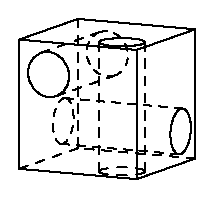
\includegraphics{asy/cube}
\end{wrapfigure}

More precisely, assume $(x,y,z)$ is the coordinate system on the cylindrical tunnel $\DD\z\times [0,1]$. 
Then the new metric is defined by
\[g=\phi\cdot [(dx)^2+ (dy)^2]+\tfrac1{\phi^2}\cdot (dz)^2,\]
where $\phi=\phi(x,y)$ is a positive smooth function on $\DD$ taking huge values around the center and equal to 1 near the boundary of $\DD$.


Gluing the opposite faces of the cube, we obtain a 3-dimensional torus with a smooth Riemannian metric.

Since the surface $S$ does not bound in $\TT^3=\mathbb{S}^1\times\mathbb{S}^1\times\mathbb{S}^1$,
one of the three coordinate projections $\TT^3\to\TT^2=\mathbb{S}^1\times\mathbb{S}^1$
induces a map of non-zero degree $S\to\TT^2$.
It follows that 
\[\area S\ge  \area(\DD,\phi\cdot [(dx)^2+ (dy)^2]).\]
For the right choice of the function $\phi$, the right hand side can be made larger than the given number $L$.
Hence the statement follows.
\qeds

I learned this problem from Dmirti Burago.
The following problem of Larry Guth \cite{guth} is closely related:

\begin{pr}
Given $\eps>0$, construct a bi-Lipschitz area-nonincreasing degree-one map 
\[[0,1]\times[0,1]\times [0,\eps]\to [0,\tfrac\eps7]\times [0,\tfrac\eps7]\times [0,\tfrac1{7\cdot\eps}].\]

\end{pr}


 
%%%%%%%%%%%%%%%%%%%%%%%%%%%%%%%%%%%%%%%%%%%%%%%%%%
\parbf{Normal exponential map.}
Assume there are $p\in M$ and $\eps>0$ 
such that the image of the normal exponential map to $L$
 does not intersect the ball $B(p,\eps)_M$; that is, no geodesic normal to $L$ crosses the ball.

Choose a positive real number $R$ such that $B(p,R)_M\cap L\ne \emptyset$.
The sectional curvature of $M$ in the ball $B(p,R)$
is bounded below by some constant, say $K$.

Given $q\in L$, denote by $v_q \in \T_qM$ the direction of a minimizing geodesic $[qp]$.
Note that $v_q\notin \mathrm{N}_qL$.
Moreover there is $\delta=\delta(\eps,K,R)\z>0$ 
such that for any point $q\in B(p,R)_M\cap L$,
and any normal vector $n\in \mathrm{N}_qL$,
we have 
\[\measuredangle (v_q,n)>\delta.\]
Otherwise the geodesic in the direction of $n$ would cross $B(p,\eps)_M$.

It follows that starting at any point $q\in B(p,R)_M\cap L$ 
one can construct a unit-speed curve $\gamma$ in $L$ such that 
\[|p-\gamma(t)|\le |p-q|-t\cdot\sin \delta.\]
Following $\gamma$ for some time brings us to $p$;
that is, $p\in L$, a contradiction.
\qeds

{

\begin{wrapfigure}{o}{28 mm}
\vskip-0 mm
\centering
\includegraphics{mppics/pic-404}
\end{wrapfigure}

The problem was suggested by Alexander Lytchak.

On the diagram you see an example of an immersion 
such that one point does not lie in the image of the corresponding normal exponential map.
It might be interesting to understand what type of subsets can be avoided by such images.

}
%%%%%%%%%%%%%%%%%%%%%%%%%%%%%%%%%%%%%%%%%%%%%%%%%%
\parbf{Symplectic squeezing in the torus.}
The embedding will be given as a composition of a linear symplectomorphism $\lambda$ 
with the quotient map $\phi\:\RR^4\to \TT^2\times\RR^2$ by the integral $(x_1,y_1)$-lattice.

\medskip

The composition $\phi\circ\lambda$ will preserve the symplectic structure;
it remains to find $\lambda$ such that the restriction $\phi\circ\lambda|_\Omega$
is injective.

Without loss of generality,
we can assume that $\Omega$ is a ball centered at the origin.
Choose an oriented 2-dimensional subspace $V$ of $\RR^4$ 
such that the integral of $\omega$ over 
$\Omega\cap V$ is a  positive number smaller than $\tfrac\pi4$. 

Note that there is a linear symplectomorphism $\lambda$ that maps planes parallel to $V$ to planes parallel to the $(x_1,y_1)$-plane, and that maps the disk $V\cap\Omega$ to a round disk.
It follows that the intersection of $\lambda(\Omega)$ 
with any plane parallel to the $(x_1,y_1)$-plane is a disk of radius at most $\tfrac 12$.
In particular $\phi\circ\lambda|_\Omega$
is injective.\qeds

This construction was given 
by Larry Guth \cite{guth-symplectic}
and attributed to Leonid Polterovich.

Note that according to Gromov's non-squeezing theorem \cite{gromov-pseudoholomorphic}, 
an analogous statement with $\CC\times \DD$ as the target space does not hold;
here $\DD\subset \CC$ is the open unit disk with the induced symplectic structure.
In particular, it shows that
the projection of $\lambda(\Omega)$ as above 
to the $(x_1,y_1)$-plane
cannot be made arbitrarily small.

%%%%%%%%%%%%%%%%%%%%%%%%%%%%%%%%%%%%%%%%%%%%%%%%%%
\parbf{Diffeomorphism test.}
Note that the map $f$ is an open immersion.

Let $h$ be the pullback metric on $M$ for $f\:M\to N$.
Clearly $h\ge g$.
In particular $(M,h)$ is complete and the map $f\:(M,h)\to N$ is a local isometry. 

Note that any local isometry between complete connected Riemannian manifolds of the same dimension is a covering map.
Since $N$ is simply connected, the result follows.
\qeds 

%???

%%%%%%%%%%%%%%%%%%%%%%%%%%%%%%%%%%%%%%%%%%%%%%%%%%
\parbf{Volume of tubular neighborhoods.}
This problem is a direct corollary of the so-called \emph{tube formula} given by Hermann Weyl \cite{weyl}.
It expresses the volume of the $r$-neighborhood of $M$ as a polynomial $p(r)$;
the coefficients of $p$, up to a multiplicative constant, are integrals over~$M$ of some quantities called the \emph{Lipschitz--Killing curvatures} --- these are certain scalars which can be expressed in terms of the curvature tensor at the given point.
The proof is done by straightforward calculations.

 

%%%%%%%%%%%%%%%%%%%%%%%%%%%%%%%%%%%%%%%%%%%%%%%%%%
%\begin{wrapfigure}[9]{r}{33 mm}
%\begin{lpic}[t(-0 mm),b(-0 mm),r(0 mm),l(0 mm)]{pics/tree(1)}
%\end{lpic}
%\end{wrapfigure}

\parbf{Disk.}
The following claim is the key step in the proof.
\begin{cl}{$({*})$}
Given a positive integer $n$, there is a binary tree $T_n$ embedded into the disk $\DD$ such that any null-homotopy of $\partial \DD$ passes a curve that intersects $n$ different edges.
\end{cl}


The proof of the claim can be done by induction on $n$; the base is trivial.
Assuming we constructed $T_{n-1}$, the tree $T_n$ can be obtained by identifying three endpoints of three copies of $T_{n-1}$.

\begin{figure}[h!]
\vskip0mm
\centering
\includegraphics{mppics/pic-406}
\end{figure}

Take $\eps=\tfrac1{10}$ and fix a large integer $n$.
Let us construct a metric on the disk $\DD$ with the embedded tree $T_n$ as in $({*})$ such that
its diameter and the length of its boundary are less than $1$
and  
the distance between any two edges of $T_n$ without a common vertex 
is at least $\eps$.

Choose a Riemannian metric $g$ on the cylinder $\mathbb S^1\times [0,1]$ such that
\begin{itemize}
\item The $\eps$-neighborhoods of the boundary components 
have product metrics.
\item Any vertical segment $x\times[0,1]$ has length $\tfrac 12$.
\item One of the boundary components has length $\eps$.
\item The other boundary component has length $2\cdot m\cdot \eps$, 
where $m$ is the number of edges in the tree $T_n$.
\end{itemize}
Equip $T_n$ with a length-metric so that each edge has length $\eps$.
Glue the cylinder $(\mathbb S^1\times [0,1],g)$ along its long boundary component to the tree $T_n$ by a piecewise isometry 
in such a way that the resulting space is homeomorphic to a disk and the obtained embedding of $T_n$ in $\DD$ is the same as in the claim $({*})$.

By $({*})$, any null-homotopy of the boundary passes a curve that intersects $n$ different edges of $T_n$.
By construction this curve is longer than $\tfrac{\eps}{10}\cdot n=\tfrac{1}{100}\cdot n$.

The obtained metric is not Riemannian, but is easy to smooth it while keeping this property.
Since $n$ is large the result follows.
\qeds
 
This example was constructed by Sidney Frankel and Mikhail Katz \cite{frankel-katz}.
 

%%%%%%%%%%%%%%%%%%%%%%%%%%%%%%%%%%%%%%%%%%%%%%%%%%
\parbf{Shortening homotopy.}
Set 
\[p=\gamma_0(0)\ \ \text{and}\ \  \ell_0=\length\gamma_0.\]

By a compactness argument,
there exists $\delta>0$ 
such that no geodesic loop based at $p$ has length in the interval $(L-D, L+D+\delta]$. 

Assume that $\ell_0\ge L+\delta$.
Choose $t_0\in [0,1]$ such that
\[\length\left(\gamma_0|_{[0,t_0]}\right)=L+\delta.\]
Let $\sigma$ be a minimizing geodesic from $\gamma(t_0)$
to $p$.
Note that $\gamma_0$ is homotopic to the concatenation 
\[\gamma_0'=\gamma_0|_{[0,t_0]}*\sigma*\bar\sigma*\gamma|_{[t_0,1]},\]
where $\bar\sigma$ denotes the backward parametrization of $\sigma$.

Applying a curve shortening process to the loop $\lambda_0=\gamma|_{[0,t_0]}*\sigma$, 
we get a  homotopy $\lambda_t$
relative to its endpoints 
from the loop $\lambda_0$ to a geodesic loop $\lambda_1$ at $p$.
From the above, 
\[\length\lambda_1\le L-D.\]

\begin{wrapfigure}{o}{29 mm}
\vskip-6mm
\centering
\includegraphics{mppics/pic-408}
\end{wrapfigure}

The concatenation $\gamma_t=\lambda_t*\bar\sigma*\gamma|_{[t_0,1]}$
is a homotopy
from $\gamma_0'$ to another curve $\gamma_1$.
From the construction it is clear that 
\begin{align*}
 \length \gamma_t&\le \length \gamma_0+2\cdot \length\sigma\le
 \\
 &\le \length \gamma_0+2\cdot D
\end{align*}
for any $t\in[0,1]$
and 
\begin{align*}
 \length \gamma_1&=\length\lambda_1+\length\sigma+\length\gamma|_{[t_0,1]}\le
\\ &\le L-D+D+\length\gamma-(L+\delta)=
\\ &=\ell_0 -\delta.
\end{align*}

Repeating the procedure sufficient number of times, we get curves $\gamma_2,\dots,\gamma_n$
connected by the needed homotopies so that 
$\ell_{i+1}\le\ell_i-\delta$ and $\ell_n\z< L+\delta$,
where $\ell_i=\length\gamma_i$.

If $\ell_n\le L$, we are done.
Otherwise repeat the argument again for $\delta'=\ell_n-L$.
\qeds

The problem is due to 
Alexander Nabutovsky 
and Regina Rotman \cite{nabutovsky-rotman}.


%%%%%%%%%%%%%%%%%%%%%%%%%%%%%%%%%%%%%%%%%%%%%%%%%%
\parbf{Convex hypersurface.}
First let us define the {}\emph{cone construction} of maps into $M$.

Let $\Delta'$ be a simplex 
with a vertex $v$.
Denote by $\Delta$ the facet in $\Delta'$ opposite to $v$.
Let $f\:\Delta\to M$ be a map such that $f(\Delta)\subset B(x,1)_M$ for some $x \in M$.
Given $w\in \Delta$, let $\gamma_w\:[0,1]\to M$ be the minimizing geodesic path from $x$ to  $f(w)$.
Since the injectivity radius of $M$ is at least $1$, the path $\gamma_w$ is uniquely defined.
The map $f'\:\Delta'\to M$ defined as 
\[f'\:(1-t)\cdot v+t\cdot w\mapsto \gamma_w(t)\] 
is called the {}\emph{cone over $f$} with vertex $x$. 

One may start with a map $f_0\:\Delta_0\to M$ and iterate the cone construction for the vertices $x_1,\dots x_k$,
to get a sequence of maps $f_i\:\Delta_i\to M$
as long as $f_{i-1}(\Delta_{i-1})\subset B(x_i,1)$.
Straightforward application of the triangle inequality 
shows that the latter conditions hold if 
$f_0(\Delta_0)\subset B(x_i,s)$ for each $i$ and $s<\tfrac2{2+k}$.

\medskip

Now we go back to the solution of the problem.

Choose a fine triangulation of $W$ so that $M$ becomes a sub-complex of $W$.
We can assume that the diameter of each simplex in $\tau$ is less than any given
$\eps>0$.
Furthermore, we can assume that all the vertices of $\tau$ can be colored with $m+2$ colors $(0,\dots, m+1)$
in such a way that the vertices of each simplex 
have different colors;
the latter can be achieved by passing to the barycentric subdivision of $\tau$.
Denote by $\tau_i$ the maximal $i$-dimensional sub-complex of $\tau$ 
with all the vertices colored by $0,\dots, i$.

Let $h$ be the maximal distance from points in $W$ to $M$.
For each vertex $v$ in $\tau$ 
choose a point $v'\in M$ at distance $\le h$.
Note that 
if $v$ and $w$ are vertices of one simplex,
then
\[|v'-w'|_M<2\cdot h+\eps.\]

Assume that $\tfrac{2}{m+3}>h$.
Choose positive $\eps<\tfrac{2}{m+3}-h$ and use it in the construction of the triangulation $\tau$ above.
Applying the iterated cone construction for each simplex of $\tau$
we get an extension of the map $v\mapsto v'$ defined on $\tau_0$ to $\tau_1,\dots\tau_{m+1}$.
According to the above estimates, the cone constructions are defined at each of the needed $m+1$ iterations.

This way we get 
to a retraction $W\to M$.
It follows that the fundamental class of $M$ vanishes in the homology ring of $M$, 
a contradiction. 
\qeds


This problem is a stripped version of the bound on filling radius given by Mikhael Gromov \cite{gromov-filling}.  

%%%%%%%%%%%%%%%%%%%%%%%%%%%%%%%%%%%%%%%%%%%%%%%%%%
\parbf{Almost constant function.}
Given a positive integer $m$,
denote by $\delta_m$ 
the expected value of $|x_1|$ for the random unit vector 
$\bm{x}\z=(x_1,\dots,x_m)\z\in\RR^m$ 
with respect to the uniform distribution.

Observe that $\delta_m\to 0$ as $m\to\infty$.
Indeed, from symmetry and Bunyakovsky inequality we get
\[
\tfrac1m=\tfrac1m\cdot\mathrm{E}(|\bm{x}|^2)
=\mathrm{E}(x_1^2)\ge \mathrm{E}(|x_1|)^2=\delta_m^2.
\]

Since $f$ is $1$-Lipschitz,
\[\mathrm{E}(|df(w)|)\le\delta_m\]
for a random vector $w$ in $\UU M$.


Note that 
\begin{align*}
|f\circ \gamma(1)-f\circ\gamma(0)|
&=
\left|\int\limits_0^1df(\gamma'(t))\cdot dt\right|\le \\
&\le \int\limits_0^1\left|df(\gamma'(t))\right|\cdot dt.
\end{align*}

Assume that $\gamma'(0)$
takes random value in $\UU M$.
By Liouville's theorem about phase volume, the same holds for $\gamma'(t)$
for any fixed $t$.
Therefore
\begin{align*}
\mathrm{E}(|f\circ \gamma(1)-f\circ\gamma(0)|)\le \mathrm{E}\left(\int\limits_0^1|df(\gamma'(t))|\cdot dt\right)\le\delta_m.
\end{align*}

By Markov's inequality,
the probability of the event 
\[|f\circ \gamma(1)-f\circ\gamma(0)|>\eps\]
is at most $\tfrac{\delta_m}{\eps}$.
Hence the result follows.
\qeds

I learned this problem from Mikhael Gromov.
It gives an example in the Riemannian world
of the so-called 
\index{concentration of measure}\emph{concentration of measure phenomenon}
\cite{milman-schechtman,ledoux}.

\csname @openrightfalse\endcsname
\chapter{Metric geometry}

In this chapter, we consider metric spaces.
All the necessary material could be found in the first three chapters of the textbook \cite{bbi}. 

Let us fix a few standard notations.
\begin{itemize}
\item The distance between two points $x$ and $y$ in a metric space $X$
will be denoted by 
\[\dist_x(y),
\quad
|x-y|
\quad\text{or}\quad
|x-y|_X,
\]
the latter notation is used to emphasize that $x$ and $y$ belong to the space $X$.
\item A metric space $X$ is called {}\emph{length-metric space} if for any two points $x,y\in X$ and any $\eps>0$, the points $x$ and $y$ can be connected by a curve $\alpha$
with
\[\length\alpha<|x-y|_X+\eps.\]
In this case we say the metric on $X$ is a \index{length-metric}\emph{length-metric}.
\end{itemize}

%%%%%%%%%%%%%%%%%%%%%%%%%%%%%%%%%%%%%%%%%
\subsection*{Embedding of a compact}
\label{compact} 

\begin{pr}
Prove that any compact metric space 
is isometric to 
a subset of a compact length-metric space.
\end{pr}

%%%%%%%%%%%%%%%%%%%%%%%%%%%%%%%%%%%%%%%%%%%%%%%%%%
\parit{Semisolution.}
Let $K$ be a compact metric space.
Denote by $\mathcal{B}(K,\RR)$ the space of real-valued bounded functions on $K$
equipped with sup-norm; 
that is, 
\[|f|=\sup\set{|f(x)|}{x\in K}.\]

Note that the map $K\to \mathcal{B}(K,\RR)$, defined by $x\mapsto \dist_x$
is a distance preserving embedding.
Indeed, by the triangle inequality we have
\[|\dist_x(z)-\dist_y(z)|\le |x-y|_K\]
for any $z\in K$
and the equality holds for $z=x$.

In other words, we can and will consider $K$ as a subspace of $\mathcal{B}(K,\RR)$.

Denote by $W$ the linear convex hull of $K$ in $\mathcal{B}(K,\RR)$;
that is, $W$ is the intersection of all closed convex subsets containing $K$. 
Clearly $W$ is a complete subspace of $\mathcal{B}(K,\RR)$.

Since $K$ is compact we can choose a finite $\eps$-net $K_\eps$ in $K$.
The set $K_\eps$ lies in a finite dimensional subspace;
therefore its convex hull $W_\eps$ is compact.
Note that $W$ lies in the $\eps$-neighborhood of $W_\eps$.
Therefore, $W$ admits a compact $\eps$-net for any $\eps>0$.
That is, $W$ is totally bounded and complete and therefore compact.

Note that line segments in $W$ are geodesics for the metric induced by the sup-norm. 
In particular $W$ is a compact length-metric space as required.
\qeds

The map $x\mapsto \dist_x$ is called the \index{Kuratowski embedding}\emph{Kuratowski embedding},
it was constructed in \cite{kuratowski}.
Essentially the same map 
was described by Maurice Fr\'echet \cite[][this is the paper where metric spaces were introduced]{frechet}.

The problem also follows directly from a theorem of John Isbell, stating that \emph{injective envelope} of compact metric space is compact;
injective envelope is an analog of convex hull in the category of metric spaces
\cite[see 2.11 in][]{isbell}.

The following related problem is open even for three-point sets.
This problem was mentioned by Mikhael Gromov [in \ncite{gromov-asymptotic},
see also \ncite{kopecka-reich} after Theorem 2.10, \ncite{convex-hull}, and Question 2.17 in \ncite{duchesne}].

\begin{pr}
Is it true that any compact subset of a complete $\CAT(0)$ length-space lies in a convex compact set?
\end{pr}


%%%%%%%%%%%%%%%%%%%%%%%%%%%%%%%%%%%%%%%%%
\subsection*{Non-contracting map\easy}
\label{Noncontracting map}

A map $f\: X\to Y$ between metric spaces is called \index{non-contracting map}\emph{distance non-contracting} if
\[|f(x)-f(x')|_Y\ge |x-x'|_X\]
for any two points $x,x'\in X$.

\begin{pr}
Let $K$  be a compact metric space and
\[f\:K\z\to K\] 
a distance non-contracting map.
Prove that $f$ is an isometry.
\end{pr}

%%%%%%%%%%%%%%%%%%%%%%%%%%%%%%%%%%%%%%%%%
\subsection*{Finite-whole extension}
\label{Finite-whole extension}

A map $f\: X\to Y$ between metric spaces is called \index{non-expanding map}\emph{non-expanding} if
\[|f(x)-f(x')|_Y\le |x-x'|_X\]
for any two points $x,x'\in X$.

\begin{pr}
Let $X$ and $Y$ be metric spaces, 
$Y$ compact,
$A\subset X$,
and $f\:A\to Y$ a non-expanding map.
Assume that for any finite set $F\subset X$ there is a non-expanding map $F \to Y$
that agrees with $f$ in $F\cap A$.
Show that there is a non-expanding map $X\to  Y$ that agrees with $f$ on $A$.
\end{pr}


%%%%%%%%%%%%%%%%%%%%%%%%%%%%%%%%%%%%%%%%%
\subsection*{Horo-compactification\easy}
\label{Horocompactification}

Let $X$ be a metric space.
Denote by $C(X,\RR)$ the space of continuous functions $X\to \RR$
equipped with the \emph{compact-open topology};
that is, for any compact set $K\subset X$ and any open set $U\subset \RR$
the set of all continuous functions $f\: X\to \RR$ such that $f(K)\subset U$
is declared to be open.

Choose a point $x_0\in X$.
Given a point $z\in X$, let $f_z\in C(X,\RR)$ be the function defined by 
\[f_z(x)=\dist_z(x)-\dist_z(x_0).\]
Let $F_X\:X\to C(X,\RR)$ be the map 
sending $z$ to $f_z$.

Denote by $\bar X$ 
the closure of $F_X(X)$ in $C(X,\RR)$;
note that $\bar X$ is compact.
That is, 
if $F_X$ is an embedding, 
then $\bar X$ is a compactification of $X$,
which is called the \index{horo-compactification}\emph{horo-compactification}.
In this case, the complement 
$\partial_\infty X\z=\bar X\backslash F_X(X)$ 
is called the {}\emph{horo-absolute} of $X$.

The construction above is due to Mikhael Gromov \cite{gromov-hyperbolic}.

\begin{pr}
Construct a proper metric space $X$
such that 
\[F_X\:X\to C(X,\RR)\] 
is not an embedding.
Show that there are no such examples among proper length-metric spaces.
\end{pr}

%%%%%%%%%%%%%%%%%%%%%%%%%%%%%%%%%%%%%%%%%
\subsection*{Approximation of the ball by a sphere}
\label{3-sphere is close to a ball}

\begin{pr}
Construct a sequence of Riemannian metrics on $\mathbb{S}^3$ converging in the sense of Gromov--Hausdorff 
to the unit ball in $\RR^3$.
\end{pr}

%%%%%%%%%%%%%%%%%%%%%%%%%%%%%%%%%%%%%%%%%
\subsection*{Macroscopic dimension\easy}
\label{macroscopic dimension} 

Let $X$ be a locally compact metric space
and $a>0$.

Following Mikhael Gromov \cite{gromov:macroscopic-dimension},
we say that the \index{macroscopic dimension}\emph{macroscopic dimension}  of $X$ at scale $a$ is the smallest integer $m$ such that there is a continuous map $f$ from $X$ to an $m$-dimensional simplicial complex $K$
with 
\[\diam[f^{-1}\{k\}]<a\]
for any point $k\in K$.

Equivalently, the macroscopic dimension of $X$ on scale $a$ can be defined as 
the smallest integer $m$ such that $X$ admits an open cover with diameter of each set less than $a$ 
and such that each point in $X$ is covered by at most $m+1$ sets in the cover.

\begin{pr}
Let $M$ be a simply connected Riemannian manifold with the following property: 
every closed curve is null-homotopic 
in its own  1-neighborhood. 
Prove that the macroscopic dimension of $M$ at scale $100$ is at most $1$.
\end{pr}

%%%%%%%%%%%%%%%%%%%%%%%%%%%%%%%%%%%%%%%%%
\subsection*{No Lipschitz embedding\hard}
\label{weird-metric} 

\begin{pr}
Construct a length-metric $d$ on $\RR^3$ such that the space $(\RR^3,d)$ does not admit a locally Lipschitz embedding into the 3-dimensional Euclidean space.
\end{pr}

%%%%%%%%%%%%%%%%%%%%%%%%%%%%%%%%%%%%%%%%%
\subsection*{Sub-Riemannian sphere\thm}
\label{sub-Riemannian} 

Let us explain what is a sub-Riemannian metric.

Let $(M,g)$ be a Riemannian manifold.
Assume that in the tangent bundle $\T M$ 
a choice of sub-bundle $H$ is given.

Let us call the sub-bundle $H$  \index{horizontal distribution}\emph{horizontal distribution}.
The tangent vectors in $H$ will be called {}\emph{horizontal}.
A piecewise smooth curve will be called {}\emph{horizontal}
if all its tangent vectors are horizontal.

The sub-Riemannian distance between any two points $x$ and $y$ is defined as the infimum of lengths of horizontal curves connecting $x$ to~$y$.

Alternatively, the distance can be defined as the limit of Riemannian distances 
for the metrics 
\[g_\lambda(X,Y)=g(X^H,Y^H)+\lambda\cdot g(X^V,Y^V)\] 
as $\lambda\to \infty$,
where $X^H$ denotes the horizontal part of $X$;
that is, the orthogonal projection of $X$ to $H$
and $X^V$ denotes the vertical part of~$X$;
so, $X^V+X^H=X$.

We also need an additional condition to ensure the following properties 
\begin{itemize}
\item The sub-Riemannian metric induces the original topology on the manifold. 
In particular, if $M$ is connected, then the distance cannot take infinite values.
\item Any curve in $M$ can be arbitrarily well approximated by a horizontal curve with the same endpoints.
\end{itemize}
The most common condition of this type is the so-called {}\emph{complete non-integrability};
it means that for any $x\in M$, 
one can choose a basis in its tangent space $\T_xM$
from the vectors of the following type
\[A(x),\quad  [A,B](x),\quad [A,[B,C]](x),\quad [A,[B,[C,D]]](x),\dots\] 
where $[{*},{*}]$ denotes the Lie bracket 
and the vector fields $A,B,C,D, \dots$ are horizontal.

\begin{pr}
Prove that any sub-Riemannian metric 
on $\mathbb{S}^m$ is isometric to the intrinsic metric of a hypersurface in $\RR^{m+1}$.
\end{pr}


It will be difficult to solve the problem without knowing a proof of the Nash--Kuiper theorem about length preserving $C^1$-embeddings.
The original papers of John Nash 
and Nicolaas Kuiper \cite{nash,kuiper} are very readable.

%%%%%%%%%%%%%%%%%%%%%%%%%%%%%%%%%%%%%%%%%
\subsection*{Length-preserving map\thm}
\label{two2one} 

A continuous map $f\:X\to Y$ between metric spaces is called \index{length-preserving}\emph{length-preserving} if it preserves the length of curves; 
that is, for any curve $\alpha$ in $X$ we have
\[\length(f\circ\alpha)=\length\alpha.\]

\begin{pr}
Show that there is no length-preserving map $\RR^2\to \RR$.
\end{pr}


The expected solution uses Rademacher's theorem \cite{rademacher} about differentiability of Lipschitz functions. 



%%%%%%%%%%%%%%%%%%%%%%%%%%%%%%%%%%%%%%%%%
\subsection*{Fixed segment}
\label{Fixed segment}

\begin{pr}
Let $\rho(x,y)=\|x-y\|$ be a metric on $\RR^m$ induced by a norm $\|{*}\|$.
Assume that $f\:(\RR^m,\rho)\to(\RR^m,\rho)$ is an isometry that fixes two distinct points $a$ and $b$.
Show that $f$ fixes the line segment between $a$ and~$b$.
\end{pr}

Evidently $f$ maps the line segment $[ab]$ to a minimizing geodesic connecting $a$ to $b$ in $(\RR^m,\rho)$.
However, in general there might be many minimizing geodesics connecting $a$ to $b$ in $(\RR^m,\rho)$.
The problem states that $[ab]$ is mapped to itself.


%%%%%%%%%%%%%%%%%%%%%%%%%%%%%%%%%%%%%%%%%
\subsection*{Pogorelov's construction\easy}
\label{Pogorelov's construction}

\begin{pr}
Let $\mu$ be a centrally symmetric Radon measure on $\mathbb{S}^2$ which is positive on every open set and vanishes on every great circle.
Given two points $x,y\in \mathbb{S}^2$,
set 
\[\rho(x,y)=\mu[B(x,\tfrac \pi2)\backslash B(y,\tfrac\pi2)].\]

Show that $\rho$ is a length-metric on $\mathbb{S}^2$
and moreover, the geodesics in $(\mathbb{S}^2,\rho)$ run along great circles of $\mathbb{S}^2$.
\end{pr}

%%%%%%%%%%%%%%%%%%%%%%%%%%%%%%%%%%%%%%%%%
\subsection*{Straight geodesics}
\label{Straight geodesics}

Recall that a map $f\:X\to Y$ between metric spaces is called bi-Lipschitz if there if a constant $\eps>0$
such that 
\[\eps\cdot|x-y|_X\le|f(x)-f(y)|_Y\le\tfrac1\eps\cdot|x-y|_X.\]
for any $x,y\in X$.

\begin{pr}
Let $\rho$ be a length-metric on $\RR^m$ that is bi-Lipschitz equivalent to the canonical metric.
Assume that every geodesic $\gamma$ in $(\RR^d,\rho)$ is \emph{affine};
that is, $\gamma(t)=v+w\cdot t$ for some $v,w\in\RR^m$.

Show that $\rho$ is induced by a norm on $\RR^m$.
\end{pr}

%%%%%%%%%%%%%%%%%%%%%%%%%%%%%%%%%%%%%%%%%
\subsection*{Hyperbolic space}
\label{Hyperbolic space}


\begin{pr}
Construct a bi-Lipschitz map
from the hyperbolic $3$-space 
to the product of two hyperbolic planes.
\end{pr}

%%%%%%%%%%%%%%%%%%%%%%%%%%%%%%%%%%%%%%%%%
\subsection*{Quasi-isometry of a Euclidean space\thm}
\label{hom-near-QI} 

A map $f\:X\to Y$ between metric spaces is called a \index{quasi-isometry}\emph{quasi-isometry} if there is a  real constant $C>1$ such that 
$$\tfrac{1}{C}\cdot|x-x'|_X-C
\le 
|f(x)-f(x')|_Y\le C\cdot|x-x'|_X+C$$
for any $x,x'\in X$ and $f(X)$ is a \index{net}\emph{$C$-net} in $Y$;
that is, for any $y\in Y$ there is $x\in X$ such that $|f(x)-y|_Y\le C$.


Note that a quasi-isometry is not assumed to be continuous;
for example any map between compact metric spaces is a quasi-isometry.

\begin{pr}
Let $f\:\RR^m\to\RR^m$ be a quasi-isometry.
Show that there is a (bi-Lipschitz) homeomorphism 
$h\:\RR^m\to\RR^m$ at a bounded distance from $f$;
that is, there is a real constant $C$ such that
$$|f(x)-h(x)|\le C$$
for any $x\in\RR^m$.
\end{pr}

The expected solution requires the so-called \emph{gluing theorem},
a corollary of the theorem proved by Laurence Siebenmann \cite{siebenmann}.
It states that 
if $V_1, V_2\subset\RR^m$ are open
and the two embedding $f_1\:V_1\to\RR^m$ and $f_2\:V_2\z\to\RR^m$ 
are sufficiently close to each other 
on the overlap $U=V_1\cap V_2$, 
then
there is an embedding $f$ defined on an open set $W'$
which is slightly smaller than $W=V_1\cup V_2$
and such that $f$ is sufficiently close to each $f_1$ and $f_2$ at the points where they are defined.

The  bi-Lipschitz version requires 
an analogous statement in the category of bi-Lipschitz embeddings;
it was proved by
Dennis Sullivan \cite{sullivan}.

%%%%%%%%%%%%%%%%%%%%%%%%%%%%%%%%%%%%%%%%%
\subsection*{Family of sets with no section\easy}
\label{hausdorff-section} 

\begin{pr}
Construct a family of closed sets $C_t\subset\mathbb{S}^1$, $t\z\in [0,1]$ that is continuous in the Hausdorff topology, 
but does not admit a {}\emph{section}.
That is, there is no path $c\:[0,1]\to \mathbb{S}^1$ such that $c(t)\in C_t$ for all $t$.
\end{pr}

\subsection*{Spaces with isometric balls}

\begin{pr}
Construct a pair of locally compact length-metric spaces $X$ and $Y$ 
that are not isometric,
but for some points $x_0\in X$,  $y_0\in Y$ and any radius $R$
the ball $B(x_0,R)_X$ is 
isometric to the ball $B(y_0,R)_Y$.
\end{pr}

\subsection*{Average distance\easy}

\begin{pr}
Show that for any compact length-metric space $X$ there is a number $\ell$ such that for any finite collection of points there is a point $z$ that lies of average distance $\ell$ from the collection;
that is, for any $x_1,\dots,x_n\z\in X$ there is $z\in X$ such that
\[\tfrac1n\cdot\sum_i|x_i-z|_{X}=\ell.\]

\end{pr}



\section*{Semisolutions}
%%%%%%%%%%%%%%%%%%%%%%%%%%%%%%%%%%%%%%%%%%%%%%%%%%



%%%%%%%%%%%%%%%%%%%%%%%%%%%%%%%%%%%%%%%%%%%%%%%%%%
\parbf{Non-contracting map.}
Given any pair of point $x_0,y_0\in K$, 
consider two sequences $x_0,x_1,\dots$ and $y_0,y_1,\dots$
such that $x_{n+1}=f(x_n)$ and $y_{n+1}=f(y_n)$ for each $n$.

Since $K$ is compact, 
we can choose an increasing sequence of integers $n_k$
such that both sequences $(x_{n_i})_{i=1}^\infty$ and $(y_{n_i})_{i=1}^\infty$
converge.
In particular, both are Cauchy sequences;
that is,
\[
|x_{n_i}-x_{n_j}|_K, |y_{n_i}-y_{n_j}|_K\to 0
\ \ 
\text{as}
\ \ \min\{i,j\}\to\infty.
\]


Since $f$ is non-contracting, we get
\[
|x_0-x_{|n_i-n_j|}|
\le 
|x_{n_i}-x_{n_j}|.
\]

It follows that  
there is a sequence $m_i\to\infty$ such that
\[
x_{m_i}\to x_0\ \ \text{and}\ \ y_{m_i}\to y_0\ \ \text{as}\ \ i\to\infty.
\leqno({*})\]

Set \[\ell_n=|x_n-y_n|_K.\]
Since $f$ is non-contracting, the sequence $(\ell_n)$ is non-decreasing.

By $({*})$,  $\ell_{m_i}\to\ell_0$ as $m_i\to\infty$.
It follows that $(\ell_n)$ is a constant sequence.

In particular 
\[|x_0-y_0|_K=\ell_0=\ell_1=|f(x_0)-f(y_0)|_K\]
for any pair of points $(x_0,y_0)$ in $K$.
That is, $f$ is distance preserving, in particular injective.

From $({*})$, we also get that $f(K)$ is everywhere dense.
Since $K$ is compact $f\:K\to K$ is surjective. Hence the result follows.\qeds


This is a basic lemma in the introduction to Gromov--Hausdorff distance \cite[see 7.3.30 in][]{bbi}.
I learned this proof from Travis Morrison, 
a student in my MASS class at Penn State, Fall 2011.

As an easy corollary one can see that any surjective non-expanding map from a compact metric space to itself is an isometry.
The following problem due to Aleksander Ca{\l}ka \cite{calka:loc-isom}
is closely related but more involved. 

\begin{pr}
Show that any local isometry from a connected compact metric space to itself is a homeomorphism. 
\end{pr}





%%%%%%%%%%%%%%%%%%%%%%%%%%%%%%%%%%%%%%%%%%%%%%%%%%
\parbf{Finite-whole extension.}
Consider the space $Y^X$ of all maps $X\to Y$ equipped with the product topology.

Given a finite set $F\in X$, denote by $\mathfrak{C}_F$ the set of maps $h\in Y^X$ such that the restriction $h|_F$ is short and the restriction $h|_{A\cap F}$ agrees with $f\:A\to Y$.
By assumption, the sets $\mathfrak{C}_F\subset Y^X$ are closed and nonempty.

Note that for any finite collection of finite sets $F_1,\dots,F_n\subset X$ we have
\[\mathfrak{C}_{F_1}\cap\dots\cap\mathfrak{C}_{F_n}\supset \mathfrak{C}_{F_1\cup\dots\cup F_n}.\]
In particular, the intersection is nonempty.

{\sloppy
According to Tikhonov's theorem \cite[see][and the references therein]{wright}, $Y^X$ is compact.
By the finite intersection propery, the intersection $\bigcap_F\mathfrak{C}_F$ with $F$ ranging along all finite subsets of $X$ is nonempty.
It remains to note that any map $h\in \bigcap_F\mathfrak{C}_F$ solves the problem.
\qeds

}

This observation was used by Stephan Stadler and me \cite{petrunin-stadler:revisited}.

%%%%%%%%%%%%%%%%%%%%%%%%%%%%%%%%%%%%%%%%%%%%%%%%%%
\parbf{Horo-compactification.}
For the first part of the problem, take $X$ to be the set of non-negative integers with the metric $\rho$ defined by
\[\rho(m,n)=m+n\] 
for $m\ne n$.

\medskip

The second part is proved by contradiction.
Assume that $X$ is a proper length space and $F_X$ is not an embedding.
That is, there is a sequence of points $z_1,z_2,\dots$ 
and a point $z_\infty$ such that $f_{z_n}\to f_{z_\infty}$ in $C(X,\RR)$
as $n\to \infty$, 
while $|z_n-z_\infty|_X>\eps$ 
for some fixed $\eps>0$ and all~$n$.

Note that any pair of points $x,y\in X$ can be connected by a minimizing geodesic $[xy]$.
Choose $\bar z_n$ on a geodesic $[z_\infty z_n]$ such that $|z_\infty-\bar z_n|=\eps$.
Note that 
\begin{align*}
f_{z_n}(z_\infty)-f_{z_n}(\bar z_n)&=\eps
\intertext{and}
f_{z_\infty}(z_\infty)-f_{z_n}(\bar z_n)&=-\eps
\end{align*}
for all $n$.

Since $X$ is proper, we can pass to a subsequence of $z_n$ so that the sequence  $\bar z_n$ converges;
denote its limit by $\bar z_\infty$.
The above identities imply that
\[f_{z_n}(\bar z_\infty)\not\to f_{z_\infty}(\bar z_\infty)
\quad
\text{or}
\quad 
f_{z_n}(z_\infty)\not\to f_{z_\infty}( z_\infty),\]
a contradiction.\qeds

I learned this problem from Linus Kramer and Alexander Lytchak;
the example was also mentioned in the lectures of Anders Karlsson
and attributed to Uri Bader \cite[see 2.3 in][]{karlsson}.





%%%%%%%%%%%%%%%%%%%%%%%%%%%%%%%%%%%%%%%%%%%%%%%%%%
\parbf{Approximation of the ball by a sphere.}
Make fine burrows in the standard 3-ball without changing its topology,
but at the same time come sufficiently close to any point in the ball.

Consider the doubling of the obtained ball along  its boundary.
The obtained space is homeomorphic to $\mathbb{S}^3$.
Note that the burrows can be made 
so that the obtained space is sufficiently close to the original ball 
in the Gromov--Hausdorff metric.

It remains to smooth the obtained space slightly 
to get a genuine Riemannian metric with the needed property.\qeds


This problem appeared as an exercise in the textbook of Dmitri Burago, Yuri Burago, and Segei Ivanov \cite[Ex. 7.5.17]{bbi}.

If $M$ is a compact manifold of dimension at least $3$
and $X$ is a reasonable compact length space,
then existence of a map $M\to X$ that induce a surjective homomorphism on their fundamental groups is a necessary and sufficient condition for existence of Gromov--Hausdorff approximation of $X$ by Riemannian metrics on $M$.
This statement was proved by Steven Ferry and Boris Okun \cite{ferry-okun}.

\begin{wrapfigure}{o}{40 mm}
\vskip-0mm
\centering
\includegraphics{mppics/pic-501}
\end{wrapfigure}

(A a doubled cone over Hawaiian earring gives an example of \emph{unreasonable} space. 
It has nontrivial fundamental group, but admits an approximation by Riemannian metrics on $\mathbb{S}^3$.)


The two-dimensional case is quite different.
There is no sequence of Riemannian metrics on
$\mathbb{S}^2$ converging to the unit disk in the sense of Gromov--Hausdorff.
In fact, 
if $X$ is a limit of $(\mathbb{S}^2,g_n)$,
then any point $x_0\in X$ either admits a neighborhood homeomorphic to $\RR^2$ or is a cut point;
that is, $X\backslash\{x_0\}$ is disconnected \cite[see 3.32 in][]{gromov-MetStr}.

%%%%%%%%%%%%%%%%%%%%%%%%%%%%%%%%%%%%%%%%%%%%%%%%%%
%%%%%%%%%%%%%%%%%%%%%%%%%%%%%%%%%%%%%%%%%%%%%%%%%%
\parbf{Macroscopic dimension.}
The following claim resembles Besicovitch inequality;
it is key to the proof.
\begin{cl}{$({*})$} Let $a$ be a positive real number.
 Assume that a closed curve $\gamma$ in a metric space $X$ can be sudivided into 4 arcs $\alpha$, $\beta$, $\alpha'$, and $\beta'$ in such a way that 
 \begin{itemize}
 \item $|x-x'|>a$ for any $x\in\alpha$ and $x'\in \alpha'$
 and
 \item $|y-y'|>a$ for any $y\in\beta$ and $y'\in \beta'$.
 \end{itemize}
 Then $\gamma$ is not contractable in its $\tfrac a2$-neighborhood.
\end{cl}


To prove $({*})$, consider two functions defined on $X$ as follows:
\begin{align*}
w_1(x)&=\min \{\,a,\dist_{\alpha}(x)\,\}
\\
w_2(x)&=\min \{\,a,\dist_{\beta}(x)\,\}
\end{align*}
and the map $\bm{w}\:X\to [0,a]\times[0,a]$, defined by
\[\bm{w}\:x\mapsto(w_1(x),w_2(x)).\]

Note that 
\begin{align*}
\bm{w}(\alpha)&=0\times [0,a],
&
\bm{w}(\beta)&=[0,a]\times 0,
\\
\bm{w}(\alpha')&=a\times [0,a],
&
\bm{w}(\beta')&=[0,a]\times a,
\end{align*} 
Therefore, the composition $\bm{w}\circ\gamma$ is a degree 1 map 
\[\mathbb{S}^1\to \partial([0,a]\times[0,a]).\] 
It follows that if $h\:\DD\to X$ shrinks $\gamma$, then there is a point $z\in\DD$ such that 
$\bm{w}\circ h(z)=(\tfrac a2,\tfrac a2)$.
Therefore $h(z)$ lies at distance at least $\tfrac a2$ from $\alpha$, $\beta$, $\alpha'$, $\beta'$
and therefore from $\gamma$.
Hence the claim $({*})$ follows.

\medskip

Choose a point $p\in M$.
Let us cover $M$ by the connected components of the inverse images 
$\dist_p^{-1}((n-1,n+1))$ for all integers $n$.
Clearly any point in $M$ is covered by at most two of these components.
It remains to show that each of these components has diameter less than $100$.

\begin{wrapfigure}{o}{31 mm}
\vskip-2mm
\centering
\includegraphics{mppics/pic-502}
\end{wrapfigure}

Assume the contrary; let $x$ and $y$ be two points in one connected component 
and $|x-y|_M\ge 100$.
Connect $x$ to $y$ with a curve $\tau$ in this component.
Consider the closed curve $\sigma$ formed by $\tau$ and two geodesics $[px]$, $[py]$.


Note that $|p-x|>40$.
Therefore there is a point $m$ on $[px]$ such that $|m-x|=20$.

By the triangle inequality, the subsdivision of $\sigma$ into the arcs $[pm]$, $[mx]$, $\tau$ and $[yp]$ satisfy the conditions of the claim $({*})$ for $a=10$.
Hence the statement follows.\qeds

The problem is due to Mikhael Gromov \cite[Appendix 1(E$_{2}$)]{gromov-filling}.

%%%%%%%%%%%%%%%%%%%%%%%%%%%%%%%%%%%%%%%%%%%%%%%%%%
\parbf{No Lipschitz embedding.}
Consider a chain of circles $c_0,\dots,c_n$ in $\RR^3$;
that is, $c_i$ and $c_{i-1}$ are linked for each $i$. 
\begin{figure}[h!]
\vskip0mm
\centering
\includegraphics{mppics/pic-504}
\end{figure}

Assume that $\RR^3$ is equipped with a length-metric $\rho$ such that the total length of the circles is $\ell$
and $U$ is an open bounded set containing all the circles $c_i$.
Note that for any $L$-Lipschitz embedding $f\:(U,\rho)\z\to\RR^3$ the distance from $f(c_0)$ to $f(c_n)$ is less than $L\cdot\ell$.

The $\rho$-distance from $c_0$ to $c_n$ might be much larger than $L\cdot\ell$.
Indeed, fix a line segment $[ab]$ in $\RR^3$.
Modify 
the length-metric on $\RR^3$ in a small neighborhood of $[ab]$
so that there is a chain $(c_i)$ of circles as above,
that goes from $a$ to $b$ 
such that
(1) the total length, say $\ell$, 
of all the circles $c_i$ is arbitrary small,
but 
(2) the obtained metric $\rho$ 
is arbitrarily close to the canonical one, say
\[\bigl|\rho(x,y)-|x-y|\bigr|<\eps\]
for any two points $x,y\in\RR^3$
and fixed in advanced small $\eps>0$.
The construction of $\rho$ 
is done by shrinking the length of each circle
and expanding the length in the normal directions  
to the circles in a small neighborhood.
The latter is made in order to make impossible to use the circles $c_i$ as a shortcut;
that is, one spends more time to go from one circle to another 
than the time one saves by going along the circle.

Set $a_n=(0,\tfrac1n,0)$ and $b_n=(1,\tfrac1n,0)$.
Note that the line segments $[a_nb_n]$ are disjoint and converging
to $[a_\infty b_\infty]$,
where $a_\infty=(0,0,0)$ and $b_\infty=(1,0,0)$.

Apply the above construction in non-overlapping convex neighborhoods of $[a_nb_n]$ 
for sequences 
$\eps_n$ and $\ell_n$ 
converging to zero very fast.

The obtained length-metric $\rho$ is still close to the canonical metric on $\RR^3$,
but it does not admit 
a locally Lipschitz homeomorphism to $\RR^3$.
Indeed, 
assume that such homeomorphism $h$ exists.
Choose a bounded open set $U$ containing $[a_\infty b_\infty]$;
note that the restriction $h|_U$ is $L$-Lipschitz for some $L$.
From the above construction,
we get 
\begin{align*}
|h(a_\infty)-h(b_\infty)|
&\le 
|h(a_n)-h(b_n)|
+
\\
&\ \ \ \ \ +
|h(a_\infty)-h(a_n)|
+
|h(b_n)-h(b_\infty)|
\le
\\
&\le
L\cdot\ell_n+\tfrac2n+100\cdot\eps_n
\end{align*}
for any positive integer $n$.
The right hand side converges to $0$ as $n\to\infty$.
Therefore 
\[h(a_\infty)=h(b_\infty),\] 
a contradiction.\qeds



The problem is due to
Dmitri Burago, 
Sergei Ivanov 
and David Shoenthal \cite{BIS}.

It is expected that any metric on $\RR^2$ admits locally Lipschitz embeddings into the Euclidean plane.
Also, it seems feasible that any metric on $\RR^3$ admits a locally Lipschitz embedding into $\RR^4$.

Note that any metric on the cube in $\RR^3$ admits a proper locally Lipschitz map to the unit cube with the canonical metric of degree 1.
Moreover one can make this map injective on any finite set of points.
It is instructive to visualize this map for the metric of the solution.

%%%%%%%%%%%%%%%%%%%%%%%%%%%%%%%%%%%%%%%%%%%%%%%%%%
\parbf{Sub-Riemannian sphere.}
If $d$ is a sub-Riemannian metric on $\mathbb{S}^m$,
then there is a non-decreasing sequence of Riemannian metric tensors
$g_0< g_1<\dots$ such that their induced metrics $d_1<d_2<\dots$ converge to $d$.
The metric $g_0$ can be assumed to be the metric of a round sphere,
so it is induced by an embedding $h_0\:\mathbb{S}^m\to \RR^{m+1}$.

Applying the construction from the Nash--Kuiper theorem,
one can produce a sequence of smooth embeddings $h_n\:\mathbb{S}^m\to \RR^{m+1}$ with the induced metrics $g_n'$
such that $|g_n'-g_n|\to 0$.
In particular, if we denote by $d'_n$ the metric corresponding to $g'_n$, then $d'_n\to d$ an $n\to\infty$.

It follows from the same construction that
if one chooses $\eps_n>0$, depending on $h_n$,
then we can assume that 
\[|h_{n+1}(x)-h_n(x)|<\eps_n\] for any $x\in \mathbb{S}^m$.

Let us introduce two conditions on the values $\eps_n$, called \emph{weak} and \emph{strong}.

The weak condition states that $\eps_{n}< \tfrac1{2}\cdot \eps_{n-1}$ for any $n$.
This ensures that the sequence of maps $h_n$ converges pointwise;
denote its limit by $h_\infty$.

Denote by $\bar d$ the length-metric induced by $h_\infty$.
Note that $\bar d\le d$.
The strong condition on $\eps_n$ will ensure that actually $\bar d=d$.

Fix $n$ and assume that $h_n$ and therefore $\eps_{n-1}$ are constructed already.
Set $\Sigma=h_n(\mathbb{S}^m)$
and let $\Sigma_r$ be the tubular $r$-neighborhood of $\Sigma$.
Equip $\Sigma$ and $\Sigma_r$ with the induced length-metrics.
Since $\Sigma$ is a smooth hypersurface, we can choose $r_n\in(0,\eps_{n-1}]$ 
so that the inclusion $\Sigma\hookrightarrow \Sigma_{r_n}$ preserves the distance up to error $\tfrac1{2^n}$.
Then the strong condition states that $\eps_n< \tfrac12\cdot r_n$, 
which is evidently stronger than the weak condition  $\eps_{n}< \tfrac1{2}\cdot \eps_{n-1}$ above.

Note that if the sequence $h_n$ is constructed with the described choice of $\eps_n$,
then $|h_\infty(x)-h_n(x)|<r_n$ for any $x\in\mathbb{S}^m$.
Therefore 
\[\bar d(x,y)+2\cdot r_n+\tfrac1{2^n}\ge d_n'(x,y)\] 
for any $n$ and $x,y\in \mathbb{S}^m$;
hence $\bar d\ge d$ as required. 
\qeds


The problem
on this list was first discovered by Enrico Le Donne \cite{le-donne}.
A similar construction is described in the lecture notes by Allan Yashinski and the author \cite{petrunin-yashinsky} 
which are aimed for undergraduate students. 
Yet the results in \cite{petrunin-paths} are closely relevant.

The construction in the Nash--Kuiper embedding theorem
can be used to prove strange statements.
Here is one example based on the observation that Weyl curvature tensor 
vanishes on hypersurfaces in the Euclidean space.

\begin{pr}
Let $M$ be a Riemannian manifold diffeomorphic to the $m$-sphere. 
Show that there is a Riemannian manifold $M'$ arbitrarily close to $M$ in the Lipschitz metric whose Weyl curvature tensor is identically 0.
\end{pr}

%%%%%%%%%%%%%%%%%%%%%%%%%%%%%%%%%%%%%%%%%%%%%%%%%%
\parbf{Length-preserving map.}
Assume the contrary;
let $f\:\RR^2\to \RR$ be a length-preserving map.

Note that $f$ is Lipschitz.
Therefore by Rademacher's theorem \cite{rademacher}, the differential $d_xf$ is defined for  almost all $x$.

Choose a unit vector $u$.
Given $x\in\RR^2$,
consider the path $\alpha_x(t)\z=x+t\cdot u$ defined for $t\in [0,1]$.
Note that  
\[\alpha'_x(t)=(d_{\alpha_x(t)}f)(u)\]
holds for almost all $x$ and $t$.
It follows that 
\[\length(f\circ\alpha_x)=\int\limits_0^1 |(d_{\alpha_x(t)}f)(u)| \cdot dt\]
for almost all $x$.

Therefore $|d_xf(v)|=|v|$ for almost all $x,v\in\RR^2$.
In particular there is $x\in\RR^2$ such that the differential $d_xf$ is defined 
and 
\[|d_xf(e_1)|=|e_1|,
\quad
|d_xf(e_2)|=|e_2|,
\quad
|d_xf(e_1+e_2)|=|e_1+e_2|\]
for a basis $(e_1,e_2)$ of $\RR^2$.
It follows that $d_xf$ has rank 2, a contradiction. \qeds 


The idea above can also be used to solve the following problem.

\begin{pr} Let $\rho$ be a metric on $\RR^2$ that is induced by a norm.
Show that $(\RR^2,\rho)$ admits 
a length-preserving map
to $\RR^3$ 
if and only if 
$(\RR^2,\rho)$ is isometric to the Euclidean plane.
\end{pr}








%%%%%%%%%%%%%%%%%%%%%%%%%%%%%%%%%%%%%%%%%%%%%%%%%%
\parbf{Fixed segment.}
Note that it is sufficient to show that 
if $f$ is an isometry such that
\[f(a)=a\ \ \text{and}\ \ f(b)=b\]
for some $a,b\in\RR^m$,
then 
\[f(\tfrac{a+b}2)=\tfrac12\cdot(f(a)+f(b)).\]


Without loss of generality, we can assume that $b+a=0$.

Set $f_0=f$.
Consider the sequence of isometries $f_0$, $f_1,\dots$ recursively defined by
\[f_{n+1}(x)= -f_n^{-1}(-f_n(x))\]
for all $n$.

Note that for all $n$ we have $f_n(a)=a$, $f_n(b)=b$ and 
$$|f_{n+1}(0)|=2\cdot|f_n(0)|.$$
Therefore  
if $f(0)\ne 0$,
then $|f_n(0)|\to\infty$ as $n\to\infty$.

On the other hand, since $f_n$ is isometry and $f(a)=a$,
we also have $|f_n(0)|\le 2\cdot |a|$, a contradiction.
\qeds

The idea of the proof is due to  Jussi V\"ais\"al\"a \cite{vaisala}.
The problem is the main step in the proof of the Mazur--Ulam theorem \cite{mazur-ulam},
which states that any isometry of $(\RR^m,\rho)$ is an affine map. 


%%%%%%%%%%%%%%%%%%%%%%%%%%%%%%%%%%%%%%%%%%%%%%%%%%

\parbf{Pogorelov's construction.}
Positivity and symmetry of $\rho$ is evident.

The triangle inequality follows since
\[[B(x,\tfrac \pi2)\backslash B(y,\tfrac\pi2)]
\cup 
[B(y,\tfrac\pi2)\backslash B(z,\tfrac\pi2)]
\supseteq
B(x,\tfrac \pi2) \backslash B(z,\tfrac\pi2).
\leqno(*)\]

\begin{wrapfigure}[8]{o}{31 mm}
\vskip-2mm
\centering
\includegraphics{mppics/pic-505}
\end{wrapfigure}

Observe that
$B(x,\tfrac \pi2)\backslash B(y,\tfrac\pi2)$
does not overlap
$B(y,\tfrac\pi2)\backslash B(z,\tfrac\pi2)$ and  we get equality in $(*)$ if and only if $y$ lies on the great circle arc from $x$ to $z$.
Therefore the second statement follows.\qeds



This construction was given by 
Aleksei Pogorelov \cite{pogorelov}.
It is closely related to the construction given 
by David Hilbert in \cite{hilbert}
which was the motivating example for his 4th problem.


%%%%%%%%%%%%%%%%%%%%%%%%%%%%%%%%%%%%%%%%%%%%%%%%%%
\parbf{Straight geodesics.}
From the uniqueness of the straight segment between two given points in $\RR^m$,
it follows that any straight line in $\RR^m$ is a geodesic in $(\RR^m,\rho)$.

Set 
\[\|\bm{v}\|_{\bm{x}}=\rho(\bm{x},(\bm{x}+\bm{v})).\]
Note that 
\[ \|\lambda\cdot\bm{v}\|_{\bm{x}}
=
|\lambda|\cdot\|\bm{v}\|_{\bm{x}}\]
for any $\bm{x},\bm{v}\in\RR^m$ and $\lambda\in\RR$.


Denote by $|x-y|$ the Euclidean distance between the points $x$ and~$y$.
Since $\rho$ and $|{*}-{*}|$ are bi-Lipschitz equivalent,
applying the triangle inequality twice to the points $\bm{x}$, $\bm{x}+\lambda\cdot\bm{v}$, $\bm{x}'$ and $\bm{x}'+\lambda\cdot\bm{v}$, we get
\[
\bigl|\|\lambda\cdot\bm{v}\|_{\bm{x}}
-
\|\lambda\cdot\bm{v}\|_{\bm{x}'}\bigr|
\le 
C\cdot |\bm{x}-\bm{x'}|\]
for any $\bm{x},\bm{x'},\bm{v}\in\RR^m$, 
$\lambda\in\RR$
and a fixed real constant $C$.

Passing to the limit as $\lambda\to\infty$, 
we obtain that
$\|\bm{v}\|_{\bm{x}}$ does not depend on $\bm{x}$;
hence the result follows.\qeds


This idea is due to Thomas Foertsch
and Viktor Schroeder \cite{foertsch-schroeder}.
A more general statement was proved by Petra Hitzelberger and Alexander Lytchak \cite{hitzelberger-lytchak}.
Namely they showed that 
if any pair of points in a geodesic metric space $X$ can be separated by an \emph{affine function},
then $X$ is isometric to a convex subset of a normed vector space.
(A function $f\:X\to\RR$ is called affine if for any geodesic $\gamma$ in $X$, the composition $f\circ\gamma$ is affine.)


%%%%%%%%%%%%%%%%%%%%%%%%%%%%%%%%%%%%%%%%%%%%%%%%%%
\parbf{Hyperbolic space.}
The hyperbolic plane $\HH^2$ is isometric to $(\RR^2,g)$, where 
\[g(x,y)=\left(\begin{matrix}
     1&0
     \\
     0&e^{x}
    \end{matrix}\right).\]
The same way, the hyperbolic space $\HH^3$
can be viewed as $(\RR^3,h)$, where 
\[h(x,y,z)=\left(\begin{matrix}
     1&0&0
     \\
     0&e^{x}&0
     \\
     0&0&e^{x}
\end{matrix}\right).\]
    
In the described coordinates, consider the projections $\phi,\psi\:\HH^3\to\HH^2$ defined by 
$\phi\:(x,y,z)\mapsto (x,y)$ and $\psi\:(x,y,z)\mapsto (x,z)$.
Note that 
\begin{align*}
\max&\{\,|\phi(p)-\phi(q)|_{\HH^2},|\psi(p)-\psi(q)|_{\HH^2}\,\}
\le
\\
&\le
|p-q|_{\HH^3}
\le
\\
&\le
|\phi(p)-\phi(q)|_{\HH^2}+ |\psi(p)-\psi(q)|_{\HH^2}
\end{align*}
for any two points $p,q\in \HH^3$.
In particular, the map $\HH^3\to\HH^2\times\HH^2$ defined by $p\mapsto (\phi(p),\psi(p))$
is $2^{\mp1}$-bi-Lipschitz.\qeds

We used that horo-spheres in the hyperbolic space are isometric to the Euclidean plane.
This observation was made by Nikolai Lobachevsky \cite[see 34 in][]{lobachevsky}.
The same observation is used in the following construction discovered by 
K\'{a}roly B\"{o}r\"{o}czky [see \ncite{boroczky} and also \ncite{radin}]. 

\begin{pr}
Construct a tessellation of the hyperbolic plane with one polygonal tile of arbitrarily small area and/or diameter.  
\end{pr}

%%%%%%%%%%%%%%%%%%%%%%%%%%%%%%%%%%%%%%%%%%%%%%%%%%
\parbf{Quasi-isometry of a Euclidean space.}
Choose two constants $M\ge 1$ and $A\ge 0$.
A map $f\:X\z\to Y$ between metric spaces $X$ and $Y$ such that for any $x,y\in X$,
 we have
\[\tfrac1M\cdot |x-y|-A\le |f(x)-f(y)|\le M\cdot |x-y|+A\]
and any point in $Y$ lies on the distance at most $A$ from a point in the image $f(X)$
will be called $(M,A)$-quasi-isometry.

{\sloppy
Note that $(M,0)$-quasi-isometry is a $[\tfrac1M,M]$-bi-Lipschitz map.
Moreover,
if $f_n\:\RR^m\to\RR^m$ is a  $(M,\frac1n)$-quasi-isometry 
for each $n$, 
then any subsequential limit of $f_n$ as $n\to\infty$
is a $[\tfrac1M,M]$-bi-Lipschitz map.

}

Therefore given $M\ge 1$ and $\eps>0$ there is $\delta>0$ such that 
for any $(M,\delta)$-quasi-isometry $f\:\RR^m\to\RR^m$ and any $p\in \RR^m$
there is an $[\tfrac1M,M]$-bi-Lipschitz map $h\:B(p,1)\to \RR^m$
such that
\[|f(x)-h(x)|<\eps\]
for any $x\in B(p,1)$.

Using rescaling, we can get the following equivalent formulation. 
Given $M\ge 1$, $A\ge 0$, and $\eps>0$,
there is sufficiently large $R>0$ such that for any $(M,A)$-quasi-isometry 
$f\:\RR^m\to\RR^m$ and any $p\in\RR^m$ there is a $[\tfrac1M,M]$-bi-Lipschitz map $h\:B(p,R)\to \RR^m$
such that 
\[|f(x)-h(x)|<\eps\cdot R\]
for any $x\in B(p,R)$.

Cover $\RR^m$ by balls $B(p_n,R)$ and construct a $[\tfrac1M,M]$-bi-Lipschitz map $h_n\:B(p_n,R)\to \RR^m$ close to the restrictions $f|_{B(p_n,R)}$ for each $n$.

The maps $h_n$ are $2\cdot \eps\cdot R$ close to each other on the overlaps of their domains of definition.
This makes possible to deform slightly each $h_n$ so that they agree on the overlaps.
This can be done by Siebenmann's theorem \cite{siebenmann}.
If instead you apply Sullivan's theorem \cite{sullivan}, you get a bi-Lipschitz homeomorphism $h\:\RR^m\z\to\RR^m$.\qeds


The problem was suggested by Dmitri Burago.





%%%%%%%%%%%%%%%%%%%%%%%%%%%%%%%%%%%%%%%%%%%%%%%%%%
\parbf{Family of sets with no section.} 
Given $t\in (0,1]$, consider the real interval $\tilde C_t=[\tfrac 1t+t, \tfrac 1t+1]$.
Denote by $C_t$ the image of $\tilde C_t$ under the covering map $\pi\:\RR\to \mathbb{S}^1=\RR/\ZZ$.

Set $C_0=\mathbb{S}^1$.
Note that the Hausdorff distance from $C_0$ to $C_t$ is $\tfrac t2$.
Therefore $\{C_t\}_{t\in[0,1]}$ is a family of compact subsets in $\mathbb{S}^1$ that is continuous in the sense of Hausdorff.

\medskip

Assume there is a continuous section $c(t)\in C_t$, for $t\in [0,1]$.
Since $\pi$ is a covering map,
we can lift the path $c$ to a path $\tilde c\:[0,1]\to \RR$ such that $\tilde c(t)\in \tilde C_t$ for all $t$.
In particular $\tilde c(t)\to\infty$ as $t\to0$,
a contradiction.\qeds


The problem was suggested by Stephan Stadler.
Here is a simpler, closely related problem.

\begin{pr}
Show that any Hausdorff continuous family of compact sets in $\RR$ admits a continuous section.
\end{pr}

The existence of sections for a family of sets parameterized by a topological space was considered by Ernest Michael \cite{michael-1,michael-2,michael-3}.

%%%%%%%%%%%%%%%%%%%%%%%%%%%%%%%%%%%%%%%%%%%%%%%%%%%%%%%%%5

\parbf{Spaces with isometric balls.} 
The needed examples can be constructed by cutting the upper half-plane along a ``dyadic comb'' shown on the diagram;
the obtained space should be equipped with the intrinsic metric induced from the $\ell_\infty$-norm on the plane. 

\medskip

First let us describe the comb precisely.
Choose an infinite sequence $a_0,a_1,\dots$ of zeros and ones.
Given an integer $k$, cut the upper half-plane along the line segment between $(k,0)$ and $(k,2^{m+1})$ 
if $m$ is the maximal number such that 
\[k\equiv a_0+2\cdot a_1+\dots+2^{m-1}\cdot a_{m-1}\pmod{2^{m}};\]
If the equality holds for all $m$, cut the half-plane along the vertical half-line starting at $(k,0)$.

\begin{wrapfigure}{o}{31 mm}
\vskip-0mm
\centering
\includegraphics{mppics/pic-506}
\end{wrapfigure}

Note that all the obtained spaces, independently from the sequence $(a_n)$, meet the conditions of the problem for the point $x_0=(\tfrac12,0)$.

Note yet that the resulting spaces for two sequences $(a_n)$ and $(a'_n)$ are isometric only in the following two cases 
\begin{itemize}
\item if $a_n=a_n'$ for all large $n$, or
\item if $a_n=1-a_n'$  for all large $n$.
\end{itemize}

It remains to produce two sequences that do not have these identities for all large $n$; 
two random sequences of zeros and ones will do the job with probability one.\qeds

%%%%%%%%%%%%%%%%%%%%%%%%%%%%%%%%%%%%%%%%%%%%%%%%%%
\parbf{Average distance.}
If such number does not exist then the ranges of average distance functions have empty intersection.
Since $X$ is a compact length-metric space, the range of any continuous function on $X$ is a closed interval.
By 1-dimesional Helly's theorem, there is a pair of such range intervals that do not intersect.
That is, for two point-arrays $(x_1,\dots,x_n)$ and $(y_1,\dots,y_m)$
and their average distance functions 
\[f(z)=\tfrac1n\cdot\sum_i|x_i-z|_X\quad\text{and}\quad h(z)=\tfrac1m\cdot\sum_j|y_j-z|_X,\] we have 
$$\min\set{f(z)}{z\in X}>\max\set{h(z)}{z\in X}.\leqno({*})$$

Note that 
$$\tfrac1m\cdot\sum_j f(y_j)=\tfrac1{m\cdot n}\cdot\sum_{i,j}|x_i-y_j|_X=\tfrac1n\cdot\sum_i h(x_i);$$
that is, the average value of $f(y_j)$ coincides with the average value of $h(x_i)$, 
which contradicts $({*})$.
\qeds

This is a result of Oliver Gross \cite{gross}. 
The value $\ell$ is called the \emph{rendezvous value} of $X$;
in fact it is uniquely defined.

\csname @openrightfalse\endcsname
\chapter{Actions and coverings}

%%%%%%%%%%%%%%%%%%%%%%%%%%%%%%%%%%%%%%%%%
\subsection*{Bounded orbit}
\label{Bounded orbit}

Recall that a metric space is called \index{proper metric space}\emph{proper} if all its bounded closed sets are compact.

\begin{pr} Let $X$ be a 
proper metric space 
and $\iota\:X\to X$ is an isometry.
Assume that for some $x\in X$, the sequence $x_n\z=\iota^n(x)$, $n\in\ZZ$ has a converging subsequence.
Prove that $x_n$ is bounded.
\end{pr}

%%%%%%%%%%%%%%%%%%%%%%%%%%%%%%%%%%%%%%%%%%%%%%%%%%
\parit{Semisolution.}
Note that we can assume that the orbit $\{x_n\}$ is dense in $X$;
otherwise pass to the closure of the orbit.
In particular, we can choose a finite number of positive integer values $n_1$, $n_2,\dots,n_k$
such that the set of points $\{x_{n_1},x_{n_2},\dots,x_{n_k}\}$ is a $\tfrac1{10}$-net for the ball $B(x_0,10)$;
that is, for any $x\in B(x_0,10)$ there is $x_{n_i}$ such that
\[|x-x_{n_i}|<\tfrac1{10}.\]

Assume $x_m\in B(x_0,1)$ for some $m$.
Then \[B(x_m,10)=f^m( B(x_0,10))\supset B(x_0,1).\] 
In particular, $\{x_{m+n_1},x_{m+n_2},\dots,x_{m+n_k}\}$ is a $\tfrac1{10}$-net for the ball $B(x_0,1)$
Therefore $x_{m+n_i}\in B(x_0,1)$ for some $i\z\in\{1,\dots,k\}$.

Set $N=\max_i\{n_i\}$.
Applying the above observation inductively, we get that from any string $x_{i+1},\dots x_{i+N}$
at least one point lies in $B(x_0,1)$.
In particular, the $N$ balls
\[B(x_1,10),\dots,B(x_N,10)\]
cover whole $X$.
Hence the result follows.\qeds

The problem is due to Aleksander Ca{\l}ka's \cite[see][]{calka}.

%%%%%%%%%%%%%%%%%%%%%%%%%%%%%%%%%%%%%%%%%
\subsection*{Finite action}\label{Finite action}

\begin{pr}
Show that for any nontrivial continuous action of a finite group on the unit sphere
there is an orbit which does not lie in the interior of a hemisphere.
\end{pr}

%%%%%%%%%%%%%%%%%%%%%%%%%%%%%%%%%%%%%%%%%


\subsection*{Covers of figure eight}\label{figure-eight-1}

Given a covering 
\[f\:\tilde X \to X\]
of the length-metric space $X$,
one can consider the induced length-metric on $\tilde X$
defining length of curve $\alpha$ in $X$ as the length of the composition $f\circ\alpha$; the obtained metric space $\tilde X$ is called \index{metric covering}\emph{metric covering} of $X$.

{

\begin{wrapfigure}[3]{r}{28 mm}
\begin{lpic}[t(-7 mm),b(-5 mm),r(0 mm),l(0 mm)]{pics/figure-eight(1)}
\end{lpic}
\end{wrapfigure}

Let us define \index{figure eight}\emph{figure eight} as the
length-metric space which
is obtained by gluing together all four ends of two unit segments.

}

\begin{pr}
Prove that any compact length-metric space $K$ 
is a Gromov--Hausdorff limit of a sequence of
metric covers  
\[(\widetilde \Phi_n, \tilde d/n)\to(\Phi,d/n),\]
where $(\Phi,d)$ denotes the figure eight.
\end{pr}


%%%%%%%%%%%%%%%%%%%%%%%%%%%%%%%%%%%%%%%%%
\subsection*{Diameter of \textit{m}-fold cover\hard}\label{m-fold-cover}

The metric covering is defined in the previous problem.

\begin{pr}
Let $X$ be a length-metric space
and $\tilde X$ be its $m$-fold metric covering of $X$.
Show that
$$\diam\tilde X\le m\cdot \diam X.$$
\end{pr}

From the diagram below you could guess an example of 5-fold cover with diameter of the total space exactly 5 times diameter of the target.

\begin{center}
\begin{lpic}[t(0mm),b(0 mm),r(0 mm),l(0 mm)]{pics/5-fold(1)}
\lbl[t]{49,4.5;$\to$}
\end{lpic}
\end{center}

%%%%%%%%%%%%%%%%%%%%%%%%%%%%%%%%%%%%%%%%%
\subsection*{Symmetric square\easy}\label{Symmetric square}

Let $X$ be a topological space.
Note that $X{\times} X$ admits a natural $\ZZ_2$-action generated by the involution $(x,y)\mapsto (y,x)$.
The quotient  space $X{\times} X/\ZZ_2$ is called \index{symmetric square}\emph{symmetric square} of $X$.

\begin{pr} 
Show that symmetric square 
of any path connected topological space 
has commutative the fundamental group.
\end{pr}

{

\begin{wrapfigure}[4]{r}{23 mm}
\begin{lpic}[t(2 mm),b(-0 mm),r(0 mm),l(0 mm)]{pics/serpinski-triangle(1)}
\end{lpic}
\end{wrapfigure}

%%%%%%%%%%%%%%%%%%%%%%%%%%%%%%%%%%%%%%%%%
\subsection*{Sierpi\'nski gasket\easy}\label{Sierpinski triangle}

To construct Sierpi\'nski gasket, start with a solid  equilateral triangle, subdivide it into four smaller congruent equilateral triangles and remove the interior of the central one.
Repeat this procedure recursively for each of the remaining solid triangles.

}

\begin{pr} 
Find the homeomorphism group of the Sierpi\'nski gasket.
\end{pr}



%%%%%%%%%%%%%%%%%%%%%%%%%%%%%%%%%%%%%%%%%
\subsection*{Lattices in a Lie group}\label{Boys and girls in a Lie group}

\begin{pr}
Let $L$ and $M$ be two discrete subgroups
of a connected Lie group $G$ and $h$ be a left
invariant metric on $G$.
Equip the groups $L$ and $M$ 
with the metrics induced from $G$.
Assume $L\backslash G$ and $M\backslash G$ are compact and
$$\vol(L\backslash (G,h))
=
\vol(M\backslash (G,h)).$$
Prove that there is a bi-Lipschitz one-to-one mapping $f\:L
\to
M$, not necessarily a homomorphism.
\end{pr}


%%%%%%%%%%%%%%%%%%%%%%%%%%%%%%%%%%%%%%%%%
\subsection*{Piecewise Euclidean quotient}\label{Piecewise Euclidean quotient}

Note that the quotient of Euclidean space by a finite subgroup of $\SO(m)$ is a {}\emph{polyhedral space} as it defined on page \pageref{piecewise linear map};
on the same page you find the definition of piecewise linear homeomorphism.


\begin{pr}
Let $\Gamma$ be a finite subgroup of $\SO(m)$.
Denote by $P$ the quotient $\RR^m/\Gamma$ equipped with induced
polyhedral metric.
Assume $P$ admits a piecewise linear homeomorphism to $\RR^m$.
Show that $\Gamma$ is generated by rotations  around subspaces of codimension $2$.
\end{pr}

%%%%%%%%%%%%%%%%%%%%%%%%%%%%%%%%%%%%%%%%%
\subsection*{Subgroups of a free group}\label{Subgroups of free group} 

\begin{pr}
Show that every finitely generated subgroup of the free group 
is an intersection of subgroups of finite index.
\end{pr}

%%%%%%%%%%%%%%%%%%%%%%%%%%%%%%%%%%%%%%%%%
\subsection*{Short generators\easy}\label{Lengths of generators of the fundamental group}

\begin{pr}
Let $M$ be a compact Riemannian manifold and $p\in M$.
Show that the fundamental group $\pi_1(M,p)$
is generated by the homotopy classes of loops with length at most $2\cdot\diam M$.
\end{pr}

%%%%%%%%%%%%%%%%%%%%%%%%%%%%%%%%%%%%%%%%%
\subsection*{Number of generators}\label{Number of generators}

\begin{pr}
Let $M$ be a complete connected Riemannian manifold with non-negative sectional curvature.
Show that the minimal number of generators of the fundamental group $\pi_1 M$
can be bounded above in terms of the dimension of $M$.
\end{pr}

%%%%%%%%%%%%%%%%%%%%%%%%%%%%%%%%%%%%%%%%%
\subsection*{Equation in a Lie group\easy}\label{Equations in the group}

\begin{pr}
Assume $G$ is a compact connected Lie group and $n$ is a positive integer.
Show that given a collection of elements $g_1,g_2\dots,g_n\in G$
the equation 
\[x\cdot g_1\cdot x\cdot g_2\cdots x\cdot g_n=1\]
has a solution $x\in G$.
\end{pr}

\section*{Semisolutions}
%%%%%%%%%%%%%%%%%%%%%%%%%%%%%%%%%%%%%%%%%%%%%%%%%%
\parbf{Finite action.}
Without loss of generality, we may assume that the action is generated by a nontrivial homeomorphism 
\[a\:\mathbb{S}^m\to\mathbb{S}^m\] 
with prime order $p$.

Assume contrary, that is, any $a$-orbit lies in an open hemisphere.
Then 
\[h(x)=\sum_{n=1}^p a^n\cdot x\ne0\]
for any $x\in\mathbb{S}^m$; here we consider $\mathbb{S}^m$ as the unit sphere in $\mathbb{R}^{m+1}$.

Consider the map $f\:\mathbb{S}^m\to\mathbb{S}^m$ 
defined as  $f(x)=\tfrac{h(x)}{|h(x)|}$.
Note that 
\begin{itemize}
\item if $a(x)=x$, then $f(x)=x$;
\item\label{f(x)=f(a(x))} $f(x)=f\circ a(x)$ for any $x\in\mathbb{S}^m$.
\end{itemize}

Note further that $f$ is homotopic to the identity; 
in particular 
\[\deg f=1.
\leqno({*})\]
The homotopy can be constructed as $(x,t)\mapsto \gamma_x(t)$,
where $\gamma_x$ is the minimizing geodesic path in $\mathbb{S}^m$ from $x$ to $f(x)$.
By construction, $|x-f(x)|_{\mathbb{S}^m}<\tfrac\pi2$; 
therefore $\gamma_x$ is uniquely defined.



Fix $x\in \mathbb{S}^m$ such that $a(x)\ne x$.
Note that the group acts without fixed points 
on the inverse image $W=f^{-1}(V)$ 
of a small open neighborhood $V\ni x$.
Therefore the quotient map $\theta\:W\to W'=W/\ZZ_p$ is a $p$-fold covering.
From  (\ref{f(x)=f(a(x))}),
the restriction $f|_W$ factors thru $\theta$;
that is,
there is $f'\:W'\to V$ such that
$f|_W=f'\circ\theta$.

Assume $p\ne 2$.
Note that $f'$ and $\theta$ have well defined degrees and 
\[\deg f\equiv\deg \theta\cdot\deg f'\pmod p\]
Since $\theta$ is a $p$-fold covering, we have $\deg \theta\equiv0\pmod p$.
Therefore
\[\deg f\equiv 0\pmod p.\leqno({*}{*})\]

Finally observe that $({*})$ contradicts $({*}{*})$.

In the case $p=2$ the same proof works, 
but the degrees have to be considered modulo $2$.\qeds

Along the same lines one can get a lower bound for the maximal diameter of orbit for any nontrivial actions of finite groups on a Riemannian manifold.

Applying the problem to the conjugate actions, 
one gets that if a fixed point set of a finite group acting on a sphere
has nonempty interior, 
then the action is trivial.
The same holds for any connected manifold.
All this was proved by Max Newman \cite[see][]{newman}.

The following problem from \cite{montgomery} can be solved using Newman's theorem. 
\begin{pr}
Assume $h$ is a homeomorphism of a connected manifold $M$ 
such that each $h$-orbit is finite.
Show that $h$ has finite order.
\end{pr}


%%%%%%%%%%%%%%%%%%%%%%%%%%%%%%%%%%%%%%%%%%%%%%%%%%
\parbf{Covers of figure eight.}
First note that any compact length-metric space $K$ can be approximated by finite metric graph.

Indeed, fix a finite $\eps$-net $F$ in $K$.
For each pair $x,y\in F$ choose a chain of points $x=x_0,x_1\dots x_n=y$ such that
$|x_i-x_{i-1}|_K<\eps$ for each $i$ and 
\[|x-y|_K=|x_0-x_1|_K+\dots+|x_{n-1}-x_n|_K.\]
Denote by $F'$ the union of all these chains with $F$;
Consider the metric graph with $F'$ as the set of vertexes
where every pair of vertexes $v$ and $w$ such that $|v-w|_K<\eps$ is connected by an edge of length $|v-w|_K$.
Note that the obtained metric graph is $\eps$ close to $K$ in the sense of Gromov--Hausdorff.

\begin{wrapfigure}{o}{27 mm}
\begin{lpic}[t(-0 mm),b(-3 mm),r(0 mm),l(0 mm)]{pics/fig8(1)}
\end{lpic}
\end{wrapfigure}

Further, any finite metric graph is a limit of metric graphs $\Gamma_n$ such that the length of each edge is a multiple of $\tfrac 1n$ and degree of each vertex is 3.

It remains to approximate $\Gamma_n$ by finite coverings of $(\Phi,d/n)$.
Guess this part from the picture; 
it shows the needed covering of figure eight for the doted graph.\qeds


The same idea works if instead of figure eight, we have any compact length-metric space $X$ which admits a map $X\to\Phi$
which is surjective on fundamental groups.
Such spaces $X$ can be found among compact hyperbolic manifolds of any dimension $\ge 2$.
All this due to Vedrin Sahovic \cite[see][]{sahovic}.

A similar idea was used later to show that any group can appear as a fundamental group of underlying space of 3-dimensional hyperbolic orbifold \cite[see][]{panov-petrunin-telescopic}.





%%%%%%%%%%%%%%%%%%%%%%%%%%%%%%%%%%%%%%%%%%%%%%%%%%
\parbf{Diameter of \textit{m}-fold cover.}
Fix points $\tilde p,\tilde q\in\tilde M$.
Let  
$\tilde\gamma\:[0,1]\to \tilde M$ be a minimizing geodesic path from $\tilde p$ to $\tilde q$. 

We need to show that 
\[\length \tilde\gamma\le m\cdot \diam M.\]
Suppose the contrary.

Denote by $p,q$ and $\gamma$ the projections to $M$ of $\tilde p,\tilde q$ and $\tilde \gamma$. 
Represent $\gamma$
as the concatenation of $m$ paths of equal length,
\[\gamma=\gamma_1{*}\dots{*}\gamma_m,\] 
so
\[\length\gamma_i=\tfrac{1}m\cdot\length\gamma>\diam M.\] 

Let $\sigma_i$ be a minimizing geodesic in $M$ connecting the endpoints of $\gamma_i$. 
Note that 
\[\length\sigma_i\le \diam M< \length\gamma_i.\] 

Consider $m+1$ paths $\alpha_0,\dots,\alpha_m$ defined as the concatenations 
\[\alpha_i=\sigma_1{*}\dots{*}\sigma_i{*}\gamma_{i+1}{*}\dots{*}\gamma_m.\]

Let $\tilde\alpha_0,\dots,\tilde\alpha_m$ be their liftings
with $\tilde q$ as the endpoint.

The staring points of $\tilde\alpha_i$ lies in one of $m$ inverse images of $p$. 
Therefore two curves, $\alpha_i$ and $\alpha_j$ for $i<j$, 
have the same starting point in $\tilde M$.

Note that the concatenation
\[\beta=\gamma_1{*}\dots{*}\gamma_i{*}\sigma_{i+1}{*}\dots{*}\sigma_j{*}\gamma_{j+1}{*}\dots{*}\gamma_m.\]
admits a lift $\tilde\beta$ 
which connects $\tilde p$ to $\tilde q$ in $\tilde M$.
Clearly $\length \tilde\beta<\length \gamma$, a contradiction.
\qeds

The question was asked by Alexander  Nabutovsky
and answered by Sergei Ivanov \cite[see][]{ivanov}.



%%%%%%%%%%%%%%%%%%%%%%%%%%%%%%%%%%%%%%%%%%%%%%%%%%
\parbf{Symmetric square.}
Let $\Gamma=\pi_1 X$ and $\Delta=\pi_1((X\times X)/\ZZ_2)$.
Consider the homomorphism $\phi\:\Gamma\times \Gamma\to \Delta$
induced by the projection $X\times X\to (X\times X)/\ZZ_2$.

Note that $\phi(\alpha,1)=\phi(1,\alpha)$ for any $\alpha\in \Gamma$ and the restrictions $\phi|_{\Gamma\times \{1\}}$ and $\phi|_{\{1\}\times\Gamma}$
are onto.

It remains to note that 
$$\phi(\alpha,1)\phi(1,\beta)=\phi(1,\beta)\phi(\alpha,1)$$
for any $\alpha$ and $\beta$ in $\Gamma$.
\qeds

 
The problem was suggested by Rostislav Matveyev.



%%%%%%%%%%%%%%%%%%%%%%%%%%%%%%%%%%%%%%%%%%%%%%%%%%
\parbf{Sierpi\'nski gasket.}
Denote the Sierpi\'nski gasket by $\triangle$.

Let us show that any homeomorphism of $\triangle$ is also its isometry.
Therefore the group homeomorphisms is the symmetric group $S_3$. 

Let $\{x,y,z\}$ be a 3-point set in $\triangle$ such that $\triangle \backslash\{x,y,z\}$ has 3 connected components.
Note that there is unique choice for the set $\{x,y,z\}$ and 
it is formed by the midpoints of its big sides.

It follows that any homeomorphism of $\triangle$ permutes the set $\{x,y,z\}$.

A similar argument shows that this permutation  uniquely describes the homeomorphism.
\qeds

The problem was suggested by Bruce Kleiner.
The homeomorphism group of Sierpi\'nski carpet is much more interesting .



%%%%%%%%%%%%%%%%%%%%%%%%%%%%%%%%%%%%%%%%%%%%%%%%%%
\parbf{Latices in a Lie group.}
Denote by $V_\ell$ and $W_m$
the Voronoi domain of for each $\ell\in L$ and $m\in M$ correspondingly;
that is,
\[V_\ell=\set{g\in G}{|g-\ell|_G\le|g-\ell'|_G\ \text{for any}\ \ell'\in L}\]
\[W_m=\set{g\in G}{|g-m|_G\le|g-m'|_G\ \text{for any}\ m'\in M}\]

Note that for any $\ell\in L$ and $m \in M$ we have
\[\begin{aligned}
\vol V_\ell&=\vol(L\backslash (G,h))=
\\
&=\vol(M\backslash (G,h))=
\\
&=\vol W_m.
\end{aligned}
\leqno({*})
\]

Consider the bipartite graph $\Gamma$ with the parts $L$ and $M$
such that $\ell\in L$ is adjacent  to $m \in M$ if and only if $V_\ell\cap W_m\ne\emptyset$.

By $({*})$ the graph $\Gamma$ satisfies the condition in the marriage theorem  ---
any subset in $L$ has at least that many neighbors in $M$ and the other way around \cite[see][]{hall}.
Therefore there is a bijection $f\: L\to M$ such that 
\[V_\ell\cap W_{f(\ell)}\ne\emptyset\] for any $\ell\in L$. 

It remains to observe that $f$ is bi-Lipschitz.
\qeds

The problem is due to 
Dmitri Burago 
and Bruce Kleiner \cite[see][]{burago-kleiner}. 
For a finitely generated group $G$  
it is not known if $G$ and $G\times \ZZ_2$ can fail to be bi-Lipschitz.
(The groups are assumed to be equipped with word metric.)
 



%%%%%%%%%%%%%%%%%%%%%%%%%%%%%%%%%%%%%%%%%%%%%%%%%%

\begin{wrapfigure}{r}{41 mm}
\begin{lpic}[t(-4 mm),b(-0 mm),r(0 mm),l(0 mm)]{pics/loop(1)}
\lbl[t]{10,-1;$x_0$}
\lbl[lb]{35,35;$\ell$}
\lbl{18,33;disc}
\end{lpic}
\end{wrapfigure}

\parbf{Piecewise Euclidean quotient.}
Note that the group $\Gamma$ serves as holonomy group of the quotient space $P=\RR^m/\Gamma$ with the induced polyhedral metric.
More precisely, one can identify $\RR^m$ with the tangent space of a regular point $x_0$ of $P$ in such a way that
for any $\gamma\in\Gamma$ there is a loop $\ell$ in $P$ which pass only thru regular points and has the holonomy $\gamma$.

Fix $\gamma$ and $\ell$ as above.
Since $P$ is simply connected, we can shrink $\ell$ by a disc.
By general position argument we can assume that the disc 
only pass thru simplices of codimension $0$, $1$ and $2$
and intersect the simplices of codimension $2$ transversely.

In other words, $\ell$ can be presented as a product of 
loops such that each loop goes around a single simplex of codimension $2$ and comes back.
The holonomy for each of these loops is a rotation around a hyperplane.
Hence the result follows.
\qeds

The converse to the problem also holds;
it was proved by Christian Lange \cite[see][]{lange};
his proof based earlier results of 
Marina Mikhailova \cite[see][]{mikhailova}.

Note that the cone over spherical suspension over Poincar\'e sphere is homeomorphic to $\RR^5$ and it is the quotient of $\RR^5$ by the binary icosahedral group, which is a subgroup of $\SO(5)$ of order 120. 
Therefore, 
if one exchanges ``piecewise linear homeomorphism'' to ``homeomorphism'' in the formulation, 
then the answer is different; 
a complete classification of such actions is given in \cite{lange}.

%%%%%%%%%%%%%%%%%%%%%%%%%%%%%%%%%%%%%%%%%%%%%%%%%%
\parbf{Subgroups of a free group.}
The proof exploits that free group is a fundamental group of graph.

\begin{wrapfigure}{r}{18 mm}
\begin{lpic}[t(-4 mm),b(-0 mm),r(0 mm),l(0 mm)]{pics/ball-in-group(1)}
\lbl[t]{8.5,7;$\tilde p$}
\lbl[t]{8.5,-2;{\small $\bar B(\tilde p,2+\tfrac12)$}}
\end{lpic}
\end{wrapfigure}

\medskip

Let $F$ be a free group and $G$ be a finitely generated subgroup in $F$.
We need to show that $G$ is an intersection of subgroups of finite index in $F$.
Without loss of generality we can assume that $F$ has finite number generators, denote it by $m$.

Let $W$ be the wedge sum of $m$ circles, 
so  $\pi_1(W,p)=F$.
Equip $W$ with the length-metric 
such that each circle has unit length.

Pass to the metric cover $\tilde W$ of $W$ 
such that  $\pi_1(\tilde W,\tilde p)=G$ 
for a lift $\tilde p$ of $p$.

Fix sufficiently large integer $n$ and consider doubling of the closed ball $\bar B(\tilde p,n+\frac12)$ along  its boundary.
Let us denote the obtained doubling by $Z_n$ and set $G_n=\pi(Z_n,\tilde p)$.

Note that $Z_n$ is a metric covering of $W$;
it makes possible to consider $G_n$ as a subgroup of $F$.
By construction, $Z_n$ is compact;
therefore $G_n$ has finite index in $F$.


It remains to show that 
\[G=\bigcap_{n>k} G_n,\]
where $k$ is the maximal length of word in the generating set of $G$.
\qeds

Originally the problem was solved by Marshall Hall \cite[see][]{hall}.
The proof presented here is close to the solution of John Stalings [see \ncite{stallings} and also \ncite{wilton}].

The same idea can be used to solve many other problems; here are some examples.
\begin{itemize}
\item {\it Show that subgroups of free groups are free.}
\item {\it Show that two elements of the free groups $u$ and $v$ commute 
if and only if they are both powers of
the some element $w$.}
\end{itemize}



%%%%%%%%%%%%%%%%%%%%%%%%%%%%%%%%%%%%%%%%%%%%%%%%%%
\parbf{Short generators.}
Choose a length minimizing loop $\gamma$ 
which represents a given element $a\in\pi_1M$.

Fix $\eps>0$.
Represent $\gamma$ 
as a concatenation
\[\gamma=\gamma_1{*}\dots{*}\gamma_n\]
of paths with $\length\gamma_i<\eps$ for each $i$.
 
Denote by $p=p_0,p_1,\dots, p_n=p$ the endpoints of these arcs.
Connect $p$ to $p_i$ by a minimizing geodesic $\sigma_i$.
Note that $\gamma$ is homotopic to a product of loops
\[\alpha_i=\sigma_{i-1}{*}\gamma_i{*}\sigma_{i-1}\]
and $\length \alpha_i<2\cdot\diam M+\eps$ for each $i$.

Given $\ell>0$, there are only finitely many elements of fundamental group which which can be realized by loops shorter than $\ell$ of at $p$.
It follows that for right choice of $\eps>0$, 
any loop $\sigma_i$ is homotopic to a loop of length at most $2\cdot\diam M$.
Hence the result follows.
\qeds

The statement is due to 
Mikhael Gromov \cite[see Proposition 3.22 in][]{gromov-MetStr}.

%%%%%%%%%%%%%%%%%%%%%%%%%%%%%%%%%%%%%%%%%%%%%%%%%%
\parbf{Number of generators.}
Consider the universal Riemannian cover $\tilde M$ of $M$.
Note that $\tilde M$ is non-negatively curved and
$\pi_1M$ acts by isometries on $\tilde M$.

Fix $p\in \tilde M$.
Given  $a\in \pi_1M$,
set 
\[|a|=|p- a\cdot p|_{\tilde M}.\]

Consider the so called \index{short basis}\emph{short basis} in $\pi_1M$;
that is, a sequence of elements $a_1,a_2,\dots\in \pi_1M$ defined the following way:
\begin{enumerate}[(i)]
\item Choose $a_1\in\pi_1M$ so that $|a_1|$ takes the minimal value.
\item Choose $a_2\in\pi_1M\backslash\langle a_1 \rangle$ so that $|a_2|$ takes the minimal value.
\item Choose $a_3\in\pi_1M\backslash\langle a_1,a_2 \rangle$ so that $|a_2|$ takes the minimal value.
\item and so on.
\end{enumerate}

Note that the sequence terminates at $n$-th step 
if 
$a_1,\dots,a_n$  generate $\pi_1M$.
By construction, we have
\begin{align*}
|a_j\cdot a_i^{-1}|&\ge |a_j|\ge |a_i|
\intertext{for any $j>i$. 
Set $p_i=a_i\cdot p$.
Note that}
|p_j-p_i|_{\tilde M}
&=|a_j\cdot a_i^{-1}|\ge
\\
&\ge |a_j|=
\\
&=|p_j-p|_{\tilde M}\ge
\\
&\ge|a_i|=
\\
&=|p_i-p|_{\tilde M}.
\intertext{By Toponogov comparison theorem we get}
\measuredangle \hinge p{p_i}{p_j}&\ge \tfrac\pi3.
\end{align*}
That is, the directions from $p$ to all $p_i$ lie on the angle at least $\tfrac\pi3$ from each other.

Therefore the number of points $p_i$ can be bounded in terms of the dimension of $M$.
Hence the result follows.
\qeds

The \emph{short basis construction} as well as the result above are due to Mikhael Gromov \cite[see][]{gromov-almost-flat}.

%%%%%%%%%%%%%%%%%%%%%%%%%%%%%%%%%%%%%%%%%%%%%%%%%%
\parbf{Equation in a Lie group.} 
We will assume that $G$ is equipped with bi-invariant metric.
In particular geodesics starting from $1\in G$ are given by homomorphisms $\RR\to G$.

Consider the map $f\:G\to G$ defined as
\[f(x)=x\cdot g_1\cdot x\cdot g_2\cdots x\cdot g_n.\]
We need to show that $f$ is onto.
Note that it is sufficient to show that $f$ has non zero degree.

The map $f$ is homotopic to the map $h\:x\mapsto x^n$.
Therefore it is sufficient to show that
\[\deg h\ne 0\leqno({*})\]

Note that the claim $({*})$ follows from $({*}{*})$.
\begin{cl}{$({*}{*})$} For any $x\in G$ the differential 
 \[d_xh\:\T_xG\to \T_{x^n}G\] 
does not revert orientation.
\end{cl}


Indeed, connect $1$ to a given point $y\in G$ by a geodesic path $\gamma$, so $\gamma(0)=1$ and $\gamma(1)=y$.
Since $\gamma\:\RR\to G$ is a homomorphism,
$h(x)=y$ for $x=\gamma(\tfrac1n)$.
In particular the inverse image $h^{-1}\{y\}$ is nonempty for any $y\in G$.

By $({*}{*})$, for a regular value $y$, each point in the  inverse image $h^{-1}\{y\}$ conributes 1 to the degree of $h$. Hence $({*})$ follows.

It remains to prove $({*}{*})$.
Given an element $g\in G$, denote by $L_g,R_g\:G\to G$ its left and right shifts;
that is, $L_g(x)=g\cdot x$ and $R_g(x)=x\cdot g$.
Identify the tangent spaces $\T_xG$ and $\T_{x^n}G$ with the Lie algebra $\mathfrak{g}=\T_eG$
using $d{R_x}\:\mathfrak{g}\to \T_xG$ and $d{R_x^n}\:\mathfrak{g}\to \T_{x^n}G$ correspondingly.
Then for any $V\in \mathfrak{g}$, we have
\[d_xh(V)=V+\Ad_x(V)+\dots+\Ad_x^{n-1}(V),\]
where $\Ad_x=d(L_x\circ R_{x^{-1}})\:\mathfrak{g}\to \mathfrak{g}$. 
Since the metric on $G$ is bi-invariant, we have $\Ad_x\in\SO(\mathfrak{g})$.
It remains to note that the linear transformation
\[V\mapsto V+T(V)+\dots+T^{n-1}(V)\]
can not revert orientation for any $T\in \SO_m$.
The last statement is an exercise in linear algebra.
\qeds

The idea of this solution is due to Murray Gerstenhaber and Oscar Rothaus 
\cite[see][]{gerstenhaber-rothaus}.
In fact the degree of $g$ is $n^k$, where $k$ is the rank of~$G$ \cite[see][]{hopf}.
\csname @openrightfalse\endcsname
\chapter{Topology}

In this chapter we consider geometrical problems with strong topological flavor.
A typical introductory course in topology, say \cite{kosniowski},
contains all the necessary material.


%%%%%%%%%%%%%%%%%%%%%%%%%%%%%%%%%%%%%%%%%
\subsection*{Isotropy}

Recall that an isotopy is a continuous one parameter family of embeddings.

\begin{pr}{}{Isotropy}\label{Isotropy}
Let $K_1$ and $K_2$ be homeomorphic compact subsets of the coordinate subspace $\RR^m$ in $\RR^{2\cdot m}$.
Show that there is a homeomorphism 
\[h\:\RR^{2\cdot m}\z\to \RR^{2\cdot m}\] 
such that $K_2=h(K_1)$.
Moreover, $h$ can be chosen to be isotopic to the identity map.
\end{pr}

%%%%%%%%%%%%%%%%%%%%%%%%%%%%%%%%%%%%%%%%%%%%%%%%%%
\parit{Semisolution.}
Fix a homeomorphism $\phi\:K_1\to K_2$.

By Tietze extension theorem,
the homeomorphisms $\phi\:K_1\to K_2$ and $\phi^{-1}\:K_2\to K_1$ can be extended to a continuous maps,
say $f\:\RR^m\to \RR^m$ and $g\:\RR^m\to \RR^m$ correspondingly.

Consider the homeomorphisms
$h_1, h_2, h_3\:\RR^m\times\RR^m\to\RR^m\times\RR^m$ defined the following way
\begin{align*}
h_1(x,y)&=(x,y+f(x)),
\\
h_2(x,y)&=(x-g(y),y),
\\ 
h_3(x,y)&=(y,-x).
\end{align*}

It remains to prove that each homeomorphism $h_i$ is isotopic to the identity map and we have $K_2=h(K_1)$ for
\[h=h_3\circ h_2\circ h_1.\]
\qedsf 

The problem is due to Victor Klee \cite[see][]{klee}.
The problem ``Monotonic homotopy'' on page \pageref{mono-homotopy} is closely related.

%%%%%%%%%%%%%%%%%%%%%%%%%%%%%%%%%%%%%%%%%
\subsection*{Immersed disks}

Two immersions $f_1,f_2\:D\looparrowright \RR^2$ are called \index{essentially different immersions}\emph{essentially different} 
if there is no diffeomorphism $h\:D\z\to D$ such that
$f_1=f_2\circ h$.

\begin{pr}{}{Immersed disks}\label{Immersed disks} 
Construct two essentially different smooth immersions of the disk 
into the plane which coincide near the boundary. 
\end{pr}

%%%%%%%%%%%%%%%%%%%%%%%%%%%%%%%%%%%%%%%%%
\subsection*{Positive Dehn twist}


Let $\Sigma$ be a surface and $\gamma\:\RR/\ZZ\to\Sigma$ be non-contractible closed simple curve.
Let $U_\gamma$ be a neighborhood of $\gamma$ which admits a homeomorphism $h\:U_\gamma\to \RR/\ZZ\times (0,1)$.
\index{Dehn twist}\emph{Dehn twist} along $\gamma$ is a homeomorphism $f\:\Sigma\z\to\Sigma$
which is identity outside of $U_\gamma$ and 
such that
$$h\circ f\circ h^{-1}\:(x,y)\mapsto(x+y,y).$$

If $\Sigma$ is oriented 
and $h$ is orientation preserving,
then the Dehn twist described above is called \index{positive Dehn twist}\emph{positive}.

\begin{pr}{\easy}{Positive Dehn twist}\label{Positive Dehn twist} Let $\Sigma$ be an oriented surface with non empty boundary.
Prove that any composition of positive Dehn twists of $\Sigma$ is not homotopic to identity rel. boundary.
\end{pr}

%%%%%%%%%%%%%%%%%%%%%%%%%%%%%%%%%%%%%%%%%
\subsection*{Function with no critical points}

\begin{pr}{}{Function with no critical points}\label{Function with no critical points}
Given an integer $m\ge 2$, 
construct a smooth function $f\:\RR^m\to \RR$ 
with no critical points in the unit ball $B^m$ 
such that the restriction $f|_{B^m}$ does not factor through a linear function;
that is, 
$f|_{B^m}$ cannot be presented as a composition
$\ell\circ\phi$,
where $\ell\:\RR^m\to\RR$ is a linear function 
and $\phi\:B^m\to\RR^m$ is a smooth embedding.
\end{pr}

%%%%%%%%%%%%%%%%%%%%%%%%%%%%%%%%%%%%%%%%%
\subsection*{Conic neighborhood}
\label{Conic neighborhood}

Let $p$ be a point in a topological space $X$.
We say that an open neighborhood $U\ni p$ is \index{conic neighborhood}\emph{conic}
if there is a homeomorphism from a cone
to $U$ which sends its vertex to $p$.

\begin{pr}{}{Conic neighborhood}  
Show that any two conic neighborhoods of one point are homeomorphic to each other.
\end{pr}

%%%%%%%%%%%%%%%%%%%%%%%%%%%%%%%%%%%%%%%%%
\subsection*{Unknots}

\begin{pr}{}{Unknots}\label{No knots}
Prove that the set of smooth embeddings $f\:\mathbb{S}^1\z\to\RR^3$ equipped with the $C^0$-topology 
forms a connected space.
\end{pr}

%%%%%%%%%%%%%%%%%%%%%%%%%%%%%%%%%%%%%%%%%
\subsection*{Stabilization}

\begin{pr}{}{Stabilization}\label{Simple stabilization}
Construct two compact subsets $K_1, K_2\subset\RR^2$ such that
$K_1$ is not homeomorphic to $K_2$, but $K_1\times[0,1]$ is homeomorphic to $K_2\z\times[0,1]$.
\end{pr}

%%%%%%%%%%%%%%%%%%%%%%%%%%%%%%%%%%%%%%%%%
\subsection*{Homeomorphism of cube}

\begin{pr}{}{Homeomorphism of cube}\label{Homeomorphism of cube}
Let $\square^m$ be a cube in $\RR^m$
and $h\:\square^m\z\to\square^m$ be
a homeomorphism which sends each face of $\square^m$ to itself.
Extend $h$ to a homeomorphism $f\:\RR^m\to\RR^m$ which coincides with the identity map outside of a bounded set.    
\end{pr}

%%%%%%%%%%%%%%%%%%%%%%%%%%%%%%%%%%%%%%%%%
\subsection*{Finite topological space\easy}


\begin{pr}{\easy}{Finite topological space}\label{Finite topological space}
Given a finite topological space $F$ 
construct a finite simplicial complex $K$
which admits a weak homotopy equivalence  $K\to F$. 
\end{pr}

%%%%%%%%%%%%%%%%%%%%%%%%%%%%%%%%%%%%%%%%%
\subsection*{Dense homeomorphism\easy}

\begin{pr}{\easy}{Dense homeomorphism}\label{Dense homeomorphism}
Let $\mathcal{H}$ be the set of all homeomorphisms $\mathbb {S}^2\to\mathbb {S}^2$ 
equipped with the $C^0$-metric.
Show that there is a homeomorphism $h\in \mathcal{H}$ such that its conjugations $a\circ h\circ a^{-1}$ for all $a\in\mathcal{H}$ form a dense set in $\mathcal{H}$.
 
\end{pr}

%%%%%%%%%%%%%%%%%%%%%%%%%%%%%%%%%%%%%%%%%
\subsection*{Simple path\easy}


\begin{pr}{\easy}{Simple path}\label{Simple path}
Let $p$ and $q$ be distinct points in Hausdorff topological space $X$.
Assume $p$ and $q$ are jointed by a path.
Show that they can be jointed by a simple path;
that is there is an injective continuous map $\beta\:[0,1]\to X$
such that $\beta(0)=p$ and $\beta(1)=q$.
\end{pr}









\section*{Semisolutions}
%%%%%%%%%%%%%%%%%%%%%%%%%%%%%%%%%%%%%%%%%%%%%%%%%%






%%%%%%%%%%%%%%%%%%%%%%%%%%%%%%%%%%%%%%%%%%%%%%%%%%
\parbf{Immersed disks.}
Both circles on the picture bound essentially different discs.

{

\begin{wrapfigure}[6]{r}{46 mm}
\begin{lpic}[t(-0 mm),b(0 mm),r(0 mm),l(0 mm)]{pics/milnors-discs()}
\end{lpic}
\end{wrapfigure}

It is a good exercise to count the discs in these examples. 
(The answers are 2 and  5 correspondingly.) 
\qeds

The first example is generally attributed to John Milnor.
The second example was given by Daniel Bennequin in \cite{bennequin}.

}

\begin{wrapfigure}[6]{r}{19 mm}
\begin{lpic}[t(-6 mm),b(0 mm),r(0 mm),l(0 mm)]{pics/annuli()}
\end{lpic}
\end{wrapfigure}

An easier problem would be to construct two essentially different immersions of annuli with the same boundary curves; a solution is shown on the picture.


%%%%%%%%%%%%%%%%%%%%%%%%%%%%%%%%%%%%%%%%%%%%%%%%%%
\parbf{Positive Dehn twist.}
Consider the universal covering 
$\tilde\Sigma\to\Sigma$.
The surface $\tilde \Sigma$ comes with the orientation induced from $\Sigma$.

Note that we may assume that $\tilde\Sigma$ has infinite number of boundary components.

Fix a point $x_0$ on the boundary of $\tilde \Sigma$.
Given other points $y$ and $z$ we will write
$y\prec z$ if $z$ lies on the left side from one (and therefore any) simple curve from $x_0$ to $y$ in $\tilde\Sigma$.
Note that  $\prec$ defines a linear order on $\partial\tilde\Sigma\backslash\{x_0\}$.
We will write $y\preceq z$ 
if $y\prec z$ or $y=z$.

\begin{center}
\begin{lpic}[t(1 mm),b(1 mm),r(0 mm),l(0 mm)]{pics/dehn()}
\lbl[t]{13,6;$x_0$}
\lbl[bl]{23,24;$y$}
\lbl[br]{4,20;$z$}
\lbl[]{33,12;$\tilde \Sigma$}
\end{lpic} 
\end{center}

Note that any homeomorphism $h\:\Sigma\to\Sigma$ which is identity on the boundary
lifts to unique homeomorphism $\tilde h\:\tilde \Sigma\to\tilde\Sigma$ 
is such a way that $\tilde h(x_0)=x_0$.

Assume $h$ is positive Dehn twist.
Show that 
$y\preceq \tilde h(y)$ for any  $y\in\partial\tilde\Sigma\backslash\{x_0\}$
and there is a point $y_0\in\partial\tilde\Sigma\backslash\{x_0\}$
such that $y_0\prec \tilde h(y_0)$.

Note that the latter property is a homotopy invariant 
and it survives under compositions of maps.
Hence the statement follows.

\parit{Comments.} The problem was suggested by Rostislav Matveyev.

%%%%%%%%%%%%%%%%%%%%%%%%%%%%%%%%%%%%%%%%%%%%%%%%%%
\begin{wrapfigure}{r}{24 mm}
\begin{lpic}[t(-0 mm),b(0 mm),r(0 mm),l(0 mm)]{pics/no-critical-points()}
\end{lpic}
\end{wrapfigure}


\parbf{Function with no critical points.}
Construct an immersion 
$\psi\:B^m\z\looparrowright\RR^m$ such that 
\[\ell\circ\phi\ne\ell\circ\psi\]
for any embedding  $\phi\:B^m\to\RR^m$. 
(The two-dimensional case can be quessed from the picture.)

It remains to note that the composition $f=\ell\circ\psi$ has no critical points.\qeds

The problem was suggested by Petr Pushkar.

%%%%%%%%%%%%%%%%%%%%%%%%%%%%%%%%%%%%%%%%%%%%%%%%%%
\parbf{Conic neighborhood.}
Let $V$ and $W$ be two conic neighborhoods of $p$.
Without loss of generality, we may assume that the closure of $V$ lies in $W$.

We will need to construct a sequence of embeddings $f_n\:V\to W$
such that 
\begin{enumerate}[(i)]
\item 
For any compact set $K\subset V$ 
there is a positive integer $n=n_K$ such that 
$f_n(k)=f_m(k)$ for any $k\in K$ and $m\ge n$.
\item For any point $w\in W$ there is a point $v\in V$ such that $f_n(v)=w$ for all large $n$.
\end{enumerate}

Note that once such sequence is constructed, $f\:V\to W$ defined as $f(v)=f_n(v)$ for all large values of $n$ gives the needed homeomorphism.

The sequence $f_n$ can be constructed recursively, setting
\[f_{n+1}=\Psi_n\circ f_n\circ \Phi_n,\]
where $\Phi_n\:V\to V$ 
and $\Psi_n\:W\to W$ 
are homeomorphisms
of the form 
\[\Phi_n(x)=\phi_n(x)\cdot x\quad \Phi_n(x)=\psi_n(x)\cdot x,\]
where $\phi_n\:V\to \RR_+$, $\psi_n\:W\to \RR_+$ are suitable continuous functions 
and 
``$\cdot$'' denotes the ``multiplication'' in the cone structures of $V$ and $W$ correspondingly.\qeds


The problem is due to Kyung Whan Kwun \cite[see][]{kwun}.

Note that for two cones $\mathop{\rm Cone}(\Sigma_1)$ and $\mathop{\rm Cone}(\Sigma_2)$ might be homeomorphic while $\Sigma_1$ and $\Sigma_2$ are not.



%%%%%%%%%%%%%%%%%%%%%%%%%%%%%%%%%%%%%%%%%%%%%%%%%%
\parbf{Unknots.}
Observe that it is possible to draw tight arbitrary knot 
while keeping it smoothly embedded all the time including the last moment.\qeds


\begin{center}
\begin{lpic}[t(-0 mm),b(0 mm),r(0 mm),l(0 mm)]{pics/knot(1)}
\end{lpic}
\end{center}


This problem was suggested by Greg Kuperberg \cite[see][]{One-step}.


%%%%%%%%%%%%%%%%%%%%%%%%%%%%%%%%%%%%%%%%%%%%%%%%%%
{
\begin{wrapfigure}{o}{37 mm}
\begin{lpic}[t(0 mm),b(0 mm),r(0 mm),l(0 mm)]{pics/Simple-stabilization(1)}
\lbl[]{8.7,8.3;{\color{white} $K_1$}}
\lbl[]{28.7,8.3;{\color{white} $K_2$}}
\end{lpic}
\end{wrapfigure}

\parbf{Simple stabilization.}
The example can be guessed from the diagram.\qeds


I learned this problem 
in my analysis class taught by 
Maria Goluzina.

}




%%%%%%%%%%%%%%%%%%%%%%%%%%%%%%%%%%%%%%%%%%%%%%%%%%
\parbf{Homeomorphism of cube.}
Let us extend the homeomorphism $h$ to whole $\RR^m$ by reflecting the cube in its facets.
We get a homeomorphism say $\tilde h\:\RR^m\to\RR^m$ such that $\tilde h(x)=h(x)$ for any $x\in\square^m$ and 
\[\tilde h\circ\gamma=\gamma\circ \tilde h\]
for any motion $\gamma\:\RR^m\to\RR^m$ in the group generated by the reflections in the facets of the cube.

Without loss of generality, we may assume that the cube $\square^m$ is inscribed in the unit sphere centered at the origin of $\RR^m$.
In this case $\tilde h$ has \index{displacement}\emph{displacement} at most $2$;
that is, 
\[|\tilde h(x)-x|\le 2\]
for any $x\in\RR^m$.

\begin{wrapfigure}[10]{o}{47 mm}
\begin{lpic}[t(-4 mm),b(0 mm),r(0 mm),l(0 mm)]{pics/Phi(1)}
\end{lpic}
\end{wrapfigure}

Fix a smooth increasing concave function $\phi\:\RR\to\RR$ such that
$\phi(r)\z=r$ for any $r\le 1$ and $\sup_r\phi(r)=2$.

Consider $\RR^m$ with polar coordinates $(u,r)$, where $u\in\mathbb{S}^{m-1}$ and $r\ge 0$.
Let $\Phi\:\RR^m\to\RR^m$
is defined by $\Phi(u,r)=(u,\phi(r))$.

Set 
\[
f(x)=\left[
\begin{aligned}
&x&&\text{if}\ |x|\ge 2
\\
&\Phi\circ \tilde h \circ \Phi^{-1}(x)&&\text{if}\ |x|< 2
\end{aligned}
\right.
\]
Prove that $f\:\RR^m\to\RR^m$ is a solution.
\qeds

The problem is a stripped from the proof of Robion Kirby in \cite{kirby}.
The condition that face is mapped to face can be removed and 
instead of homeomorphism one can take an embedding which is close enough to the identity.

An interesting twist to this idea was given by Dennis Sullivan in \cite{sullivan}.
Instead of the discrete group of motions of Euclidean space,
he use a discrete group of motions of hyperbolic space in the Poincare model.
Say, assume we repeat the same argument if instead of cube we have a Coxeter polytope in the hyperbolic space.
Then the constructed map 
coincides with the identity on the absolute and therefore the last ``shrinking'' step in the proof above is not needed.
Moreover, 
if the original homeomorphism is bi-Lipschitz,
then the construction also produce a bi-Lipschitz homeomorphism;
this is the advantage.
  

%%%%%%%%%%%%%%%%%%%%%%%%%%%%%%%%%%%%%%%%%%%%%%%%%%
\parbf{Finite topological space.}
Given a point $p\in F$,
denote by $O_p$ the minimal open set in $F$ containing $p$. 
Note that we can assume that $F$ connected and is $T_0$;
that is $O_p=O_q$ if and only if $p=q$.

Let us write $p\preccurlyeq q$ 
if $O_p\subset O_q$.
The relation $\preccurlyeq$ is a partial order on $F$.

Let us construct a simplicial complex $K$ 
by taking $F$ as the set of its vertices
and saying that a collection of vertices form a simplex 
if they can form a an increasing sequence with respect to $\preccurlyeq$.

Given $k\in K$,
consider the minimal simplex $(f_0,\dots,f_m)\ni k$;
we can assume that $f_0\preccurlyeq \dots\preccurlyeq f_m$.
Set $h\:k\mapsto f_0$;
it defines a map $K\to F$.

It remains to check that $h$ is continuous 
and induces an isomorphism of all the homotopy groups.
\qeds

In a similar fashion, one can construct a finite topological space $F$ for given simplicial complex $K$ 
such that 
there is a weak homotopy equivalence $K\to F$.
Both constructions are due to Pavel Alexandrov, 
\cite[see][]{alexandrov-finite,mccord}.

\parbf{Dense homeomorphism.}
Note that there is countable set of homeomorphisms $h_1,h_2,\dots$ which is dense in $\mathcal{H}$
such that
each $h_n$ fix all the points outside an open round disc, say $D_n$.

Choose a countable disjoint collection of round discs $D_n'$
and consider the homeomorphism $h\:\mathbb S^2\to \mathbb S^2$
which fix all the points outside of $\bigcup_nD'_n$ and
for each $n$,
the restriction $h|_{D_n'}$ is conjugate to $h_n|_{D_n}$. 

Show that $h$ solves the problem.
\qeds

The problem was mentioned by Frederic Le Rox \cite[see][]{rox}.

%%%%%%%%%%%%%%%%%%%%%%%%%%%%%%%%%%%%%%%%%%%%%%%%%%
\parbf{Simple path.}
Let $\alpha$ be a path joining $p$ to $q$.

Passing to a subinterval if necessary,
we can assume that $\alpha(t)\ne p,q$ for $t\ne0,1$.

An open set in $[0,1]$ will be called {}\emph{suitable}
if for any connected component $(a,b)$ of $\Omega$ we have $\alpha(a)=\alpha(b)$.
Show that there is a maximal suitable open set $\Omega$;
that $\Omega$ is suitable and it is not a subset of any other suitable set.

Define $\beta(t)=\alpha(a)$ for any $t$ in a connected component $(a,b)\subset\Omega$.

It remains to reparametrize $\beta$ to make it injective.
\qeds

The problem inspired by a Lemma 7.13 
proved by 
Alexander Lytchak
and Stefan Wenger in \cite{lytchak-wenger}

A more involved solution goes the following way:
Note that one can assume that $X$ coincides with the image of $\alpha$.
In particular it is connected, locally connected and compact.

Any such space admits a length metric.
This statement was conjectured by Karl Menger in \cite{menger}
and proved independently 
by R. H. Bing  \cite[see][]{bing-length-0, bing-length-1} 
and Edwin Moise \cite[see][]{moise}.

It remains to consider a geodesic path from $p$ to $q$.
\csname @openrightfalse\endcsname
\chapter{Piecewise linear geometry}


A \index{polyhedral space}\emph{polyhedral space} is a complete length-metric space that admits a locally finite triangulation 
such that each simplex is isometric to a simplex in a Euclidean space.
By a {}\emph{triangulation} of a polyhedral space we always understand it as a triangulation as above. 

A point in a polyhedral space is called \index{regular point}\emph{regular} if it has a neighborhood isometric to an open set in a Euclidean space;
otherwise it is called {}\emph{singular}.

If we replace the Euclidean spaces by the unit spheres or the hyperbolic spaces,
we arrive to the definition of {}\emph{spherical} and {}\emph{hyperbolic polyhedral spaces} correspondingly.

The term \index{piecewise}\emph{piecewise} typically mean that there is a triangulation with some property on each triangle.
For example,  if $P$ and $Q$ are polyhedral spaces, then
\begin{itemize}
\item a map $f\:P\to Q$ is called {}\emph{piecewise distance preserving} if there is a triangulation $\mathcal{T}$ of $P$ such that for any simplex $\Delta\in \mathcal{T}$ the restriction $f|_\Delta$ is distance preserving,
\item a map $h\:P\z\to Q$  is called {}\emph{piecewise linear} if both spaces $P$ and $Q$ admit triangulations such that each simplex of $P$ is mapped to a simplex of $Q$ by an affine map.
In particular, a {}\emph{piecewise linear homeomorphism} is a piecewise linear map which is a homeomorphism.\label{piecewise linear map}
\end{itemize}





%%%%%%%%%%%%%%%%%%%%%%%%%%%%%%%%%%%%%%%%%
\subsection*{Spherical arm lemma}\label{Spherical arm lemma}

Recall that a polygon without self intersections is called \index{simple polygon}\emph{simple}.

\begin{pr}
Let $A=[a_1\dots a_n]$ and $B=[b_1\dots b_n]$ be two simple spherical polygons 
with equal corresponding sides.
Assume $A$ lies in a hemisphere and $\measuredangle a_i\ge\measuredangle b_i$ for each $i$.
Show that $A$ is congruent to $B$.
\end{pr}

%%%%%%%%%%%%%%%%%%%%%%%%%%%%%%%%%%%%%%%%%%%%%%%%%%
\parit{Semisolution.}
Let us cut the polygon $A$ from the sphere and glue instead the polygon $B$.
Denote by $\Sigma$ the obtained spherical polyhedral space.
Note that 
\begin{itemize}
\item $\Sigma$ is homeomorphic $\mathbb S^2$.
\item $\Sigma$ has curvature $\ge 1$ in the sense of Alexandrov; that is, the total angle around each singular point is less than $2\cdot \pi$.
\item All the singular points of $\Sigma$ 
lie outside of an isometric copy of a hemisphere $\mathbb{S}^2_+\subset \Sigma$
\end{itemize}

Denote by $n$ the number of singular points in $\Sigma$.
It is sufficient to show that $n=0$.

Assume the contrary; that is, $n\ge 1$.
We can assume that $n$ takes the minimal possible value.

Clearly $n>1$;
that is, $\Sigma$ can not have a single singular point.
Therefore we can choose two singular points $p,q\in \Sigma$.
Cut $\Sigma$ along a geodesic $[pq]$.
The hole can be patched so that we obtain a new polyhedral space $\Sigma'$ of the same type but with $n-1$ singular points.
Since $n$ is minimal, we arrive to a contradiction

Namely, if the total angles around $p$ and $q$ are $2\cdot \pi-\alpha$ and $2\cdot \pi-\beta$ correspondingly,
consider the spherical triangle $\triangle$ with base $|p-q|_\Sigma$ and adjusted angles $\tfrac\alpha2$, $\tfrac\beta2$. 
The needed patch is obtained by doubling $\triangle$ along its lateral sides.
\qeds

\parit{Alternative end of proof.}
By the Alexandrov embedding theorem, $\Sigma$ is isometric to the surface of a convex polyhedron $P$ in the unit 3-dimensional sphere $\mathbb S^3$. 
The center of the hemisphere has to lie in a facet, say $F$ of $P$.
It remains to note that $F$ contains the equator and therefore $P$ has to be a hemisphere in $\mathbb S^3$ or an intersection of two hemispheres.
In both cases its surface is isometric to $\mathbb S^2$.
\qeds

The problem is due to Victor Zalgaller \cite[see][]{zalgaller-shperical-polygon};
the result of Victor Toponogov in \cite{toponogov} gives a smooth analog of this statement.
The patch construction above was introduced by 
Aleksandr Alexandrov
in his proof of convex embeddability of polyhedra
\cite[see][VI, \S7]{alexandrov1948}.
The alternative end of proof is taken from \cite{panov-petrunin}.



%%%%%%%%%%%%%%%%%%%%%%%%%%%%%%%%%%%%%%%%%
\subsection*{Triangulation of 3-sphere}\label{4-poly}

\begin{pr}
Construct a triangulation of $\mathbb{S}^3$ 
with $100$ vertices
such that any two vertices are connected by an edge.
\end{pr}

%%%%%%%%%%%%%%%%%%%%%%%%%%%%%%%%%%%%%%%%%
\subsection*{Folding problem}\label{Folding problem}

\begin{pr}
Let $P$ be a compact $2$-dimensional 
polyhedral space. 
Construct a 
piecewise distance preserving map
$f\:P\to \RR^2$.
\end{pr}

%%%%%%%%%%%%%%%%%%%%%%%%%%%%%%%%%%%%%%%%%
\subsection*{Piecewise distance preserving extension}\label{iso-kirzhbraun}

\begin{pr}
Prove that any 1-Lipschitz map from a finite subset $F\subset \RR^2$
to 
$\RR^2$ can be extended to a 
piecewise distance preserving map
$\RR^2\to\RR^2$.
\end{pr}

%%%%%%%%%%%%%%%%%%%%%%%%%%%%%%%%%%%%%%%%%
\subsection*{Closed polyhedral surface}\label{Closed polyhedral surface}

\begin{pr}
Construct a closed polyhedral surface $\Sigma$ in $\RR^3$ with nonpositive curvature;
that is, the total angle around each vertex of $\Sigma$ is at least $2\cdot\pi$.
\end{pr}

%%%%%%%%%%%%%%%%%%%%%%%%%%%%%%%%%%%%%%%%%
\subsection*{Minimal polyhedral disk}\label{Minimal polyhedral disk}

By a polyhedral disk in $\RR^3$
we understand a triangulation of a plane polygon $P$ with a map $P\to\RR^3$ that is affine on each triangle.
The area of the polyhedral disk is defined as the sum of areas of the images of the triangles in the triangulation.

\begin{pr}
Consider the  class of polyhedral disks glued from $n$ triangles in $\RR^3$ 
with fixed broken line as the boundary.
Let $\Sigma_n$ be a disk of minimal area in this class.
Show that $\Sigma_n$ is  \index{saddle surface}\emph{saddle};
that is, a plane can not cut all the edges coming from one of the interior vertices of $\Sigma_n$.
\end{pr}

%%%%%%%%%%%%%%%%%%%%%%%%%%%%%%%%%%%%%%%%%
\subsection*{Coherent triangulation\easy}\label{Coherent triangulation} 

A triangulation of a convex polygon is called coherent if there is a convex function that is linear on each triangle and changes its gradient on every edge of the triangulation.

\begin{pr}
Find a non-coherent triangulation of a triangle.
\end{pr}



%%%%%%%%%%%%%%%%%%%%%%%%%%%%%%%%%%%%%%%%%
\subsection*{Sphere with one edge\hard}\label{panov-S^3} 

Given  a polyhedral space $P$,
denote by $P_s$ the set of its 
singular points.

\begin{pr}
Construct spherical polyhedral space $P$ that is homeomorphic to $\mathbb{S}^3$ and such that $P_s$ is formed by a knotted circle.
\end{pr}

In addition the total length of $P_s$ can be made arbitrary large and the angle around $P_s$ can be made strictly less than $2\cdot\pi$.

%%%%%%%%%%%%%%%%%%%%%%%%%%%%%%%%%%%%%%%%%
\subsection*{Triangulation of a torus}\label{Triangulation of a torus}

\begin{pr}
Show that the torus does not admit a triangulation 
such that one vertex has 5 edges,
one has 7 edges and 
all other vertices have 
6 edges. 
\end{pr}


%%%%%%%%%%%%%%%%%%%%%%%%%%%%%%%%%%%%%%%%%
\subsection*{No simple geodesics\easy}\label{No simple geodesics}

\begin{pr}
Construct a convex polyhedron $P$ whose surface 
does not have a closed simple geodesic.
\end{pr}

\section*{Semisolutions}
%%%%%%%%%%%%%%%%%%%%%%%%%%%%%%%%%%%%%%%%%%%%%%%%%%


%%%%%%%%%%%%%%%%%%%%%%%%%%%%%%%%%%%%%%%%%%%%%%%%%%
\parbf{Triangulation of 3-sphere.}
Choose 100 distinct points $p_1\z\dots,p_{100}$
on the {}\emph{moment curve} 
\[\gamma\:t\mapsto (t,t^2,t^3,t^4)\] 
in $\RR^4$.
Denote by $P$ the convex hull of $\{p_1,\z\dots,p_{100}\}$.

The surface of $P$ is homeomorphic to $\mathbb{S}^2$.
Therefore it is sufficient to show that any two vertices of $P$ are connected by an edge.
The latter follows from the following claim.

\begin{cl}{$({*})$}
For any two points $p$ and $q$ on $\gamma$ there is a hyperplane $H$ in $\RR^4$ which intersects $\gamma$ only at $p$ and $q$ and leaves $\gamma$ on one side.
\end{cl}

To prove the claim, assume that $p=\gamma(t_1)$ and $q=\gamma(t_2)$. 
Consider the polynomial
\[f(t)=a+b\cdot t+c\cdot t^2+d\cdot t^3+t^4=(t-t_1)^2\cdot(t-t_2)^2.\]
Clearly $f(t)\ge 0$ and the equality holds only at $t_1$ and $t_2$.
It follows that the affine function $\ell\:\RR^4\to\RR$ defined as 
\[\ell\:(w,x,y,z)\mapsto a+b\cdot w+c\cdot x+d\cdot y+z\]
is nonnegative at the points of $\gamma$ and vanish only at $p$ and $q$.
Therefore the zero set of $\ell$ is the required hyperplane $H$ in $({*})$. 
\qeds

The polyhedron $P$ above is an example of the so called \index{cyclic polytope}\emph{cyclic polytopes}.

%%%%%%%%%%%%%%%%%%%%%%%%%%%%%%%%%%%%%%%%%%%%%%%%%%
\parbf{Folding problem.}
Given a triangulation of $P$,
consider the Voronoi domain $V_v$ for each vertex $v$;
that is, $V_v$ is the set of all points in $P$ closer to $v$ than to any other vertex.
Note that the triangulation can be subdivided if necessary
so that the Voronoi domain of each vertex is isometric to a convex subset in the cone with the vertex corresponding to the tip.

The boundaries of all the Voronoi domains form a graph with straight edges.
Let us triangulate $P$ so that each triangle has one of those edges as the base 
and the opposite vertex is the center of an adjusted Voronoi domain; 
such a vertex will be called the {}\emph{main} vertex of the triangle.


\begin{wrapfigure}[8]{o}{43 mm}
\begin{lpic}[t(-0 mm),b(0 mm),r(0 mm),l(0 mm)]{pics/zalgaller(1)}
\lbl[tl]{12.5,13.5;$v$}
\lbl[tr]{36.5,24;$w$}
\lbl[l]{33.5,2;$a$}
\lbl[b]{21,34;$b$}
\lbl[tl]{22,17;$x$}
\lbl{26,11;$\triangle$}
\lbl[w]{11,8;$V_v$}
\lbl[w]{36,30;$V_w$}
\lbl[tl]{17,17;$\rho$}
\lbl[bl]{17,19;{\small $\theta$}}
\end{lpic}
\end{wrapfigure}

Fix a solid triangle $\triangle=[vab]$ in the constructed triangulation; 
let $v$ be its main vertex.
Given a point 
$x\in  \triangle$, set 
\begin{align*}
\rho(x)&=|x-v|
\intertext{and}
\theta(x)&=\min \{\measuredangle \hinge vax,\measuredangle\hinge vbx\}.
\end{align*}
Let us map $x$ to the point with polar coordinates $(\rho(x),\theta(x))$ in the plane.

Note that for each triangle $\triangle$, 
the constructed map $\triangle\to\RR^2$ is piecewise distance preserving.
It remains to check that these maps agree on the common sides of the triangles.
\qeds


This construction was given by Victor Zalgaller \cite[see][]{zalgaller-polyhedra}.
Svetlana Krat generalized the statement to higher dimensions \cite[see][]{krat}.



%%%%%%%%%%%%%%%%%%%%%%%%%%%%%%%%%%%%%%%%%%%%%%%%%%
\parbf{Piecewise distance preserving extension.}
Let $a_1,\dots,a_n$
and $b_1,\z\dots,b_n$
be two collections of points in $\RR^2$
such that 
\[|a_i-a_j|\ge |b_i-b_j|\] 
for all pairs $i$, $j$.
We need to construct a piecewise distance preserving map $f\:\RR^2\to\RR^2$
such that $f(a_i)=b_i$ for each $i$.

Assume that the problem is already solved for $n<m$;
let us do the case $n=m$.
By assumption, 
there is a piecewise liner length-preserving map $f\:\RR^2\to\RR^2$
such that $f(a_i)=b_i$ for each $i>1$.

Consider the set 
\[\Omega=\set{x\in\RR^2}{|f(x)-b_1|>|x-a_1|}.\]
Since $|a_i-a_1|\ge|b_i-b_1|$, we get $a_i\notin \Omega$ for $i>1$.

Note that we can assume that the map $f$ and therefore the set $\Omega$ are bounded.
Indeed, let $\square$ be a square containing all the points $b_i$.
There is a piecewise isometric map $h\:\RR^2\to\square$ obtained by folding plane along the lines of the grid defined by $\square$.
Then the composition $h\circ f$ is bounded and it satisfies all the properties of $f$ described above.

If $\Omega=\emptyset$,
then $f(a_1)=b_1$; 
that is, $f$ is a solution.
It remains to consider the case $\Omega\ne\emptyset$. 

Note that $\Omega$ is star-shaped with respect to $a_1$.
Indeed, if $x\in \Omega$, then $|a_1-x|<|b_1-f(x)|$.
If $y\in [a_1x]$ then 
$|a_1-y|+|y-x|=|a_1-x|$ and since $f$ is length-preserving we get $|f(x)-f(y)|\le |x-y|$.
By the triangle inequality, 
$|a_1-y|<|b_1-f(y)|$; that is, $y\in\Omega$. 



\begin{wrapfigure}{r}{40 mm}
\begin{lpic}[t(-0 mm),b(0 mm),r(0 mm),l(0 mm)]{pics/star(1)}
\lbl{11,11;$\Omega$}
\lbl[t]{21,9.5;$a_1$}
\lbl[bl]{17,26.3,-36;$E_i$}
\lbl{20,19;$T_i$}
\end{lpic}
\end{wrapfigure}

The boundary $\partial\Omega$ can be subdivided into a finite collection of line segments $\{E_i\}$
so that $f$ maps rigidly each $E_i$.
Note that $|f(x)\z-b_1|=|x-a_1|$ for any $x\in E_i$.
Denote by $T_i$ the triangle with base $E_i$ and vertex $a_1$.
From above there is a rigid motion $m_i$ of $T_i$ such that $m_i(x)=f(x)$ for any $x\in E_i$ and $m_i(a_1)=b_1$.
Let us redefine the map $f$ in $\Omega$ by sending $x$ to $m_i(x)$ for $x\in T_i$.

The maps $m_i$ agree on the common sides of triangles $T_i$.
Therefore we have produced a new piecewise isometric map $f'\:\RR^2\to \RR^2$ satisfying all the requirements.
\qeds

The same proof works in all dimensions.

The statement was proved by Ulrich Brehm 
and rediscovered by Arseniy Akopyan and Alexey Tarasov [see \ncite{brehm}, \ncite{akopyan-tarasov} and also the section 2 in \ncite{petrunin-yashinsky}].

%%%%%%%%%%%%%%%%%%%%%%%%%%%%%%%%%%%%%%%%%%%%%%%%%%

\begin{wrapfigure}{o}{37 mm}
\begin{lpic}[t(-0 mm),b(-3 mm),r(0 mm),l(0 mm)]{pics/octahedron-with-holes(1)}
\end{lpic}
\end{wrapfigure}

\parbf{Closed polyhedral surface.}
An example can be constructed by drilling a polyhedral cave from your favorite convex polyhedron.
On the diagram you see the result of this construction for the octahedron.

\medskip

Choose a convex polyhedron $K$.
We can assume that the interior of $K$ contains the origin $0\in\RR^3$.
Remove from $K$ the interior of $K'=\tfrac56\cdot K$.

Note that one can drill from each vertex of $K$ a polyhedral tunnel to the corresponding vertex of $K'$
so that the surface $\Sigma$ of the obtained non-convex polytope is a solution.
\qeds

The problem suggested by Jaros{\l}aw K\k{e}dra.

The construction above produces a surface of genus at least 3.
One can also construct a polyhedral surface in $\RR^3$
which is isometric to a flat torus.
The existence of such torus follows from very general result of Burago and Zalgaller \cite[see][]{burago-zalgaller:pl}.
They show in particular that any 1-Lipschitz smooth embedding of the flat torus in $\RR^3$ can be approximated by a piecewise distance preserving embedding.

\begin{wrapfigure}[4]{r}{20 mm}
\begin{lpic}[t(-4 mm),b(0 mm),r(0 mm),l(0 mm)]{pics/cylinder(1)}
\end{lpic}
\end{wrapfigure}

The following construction is more direct;
it is a bent version of the so called \index{Schwarz boot}\emph{Schwarz boots} \cite[see][]{schwarz1890definition}.
Construct an isometric piecewise linear embedding of a cylinder $\SSS^1\times [0,a]$ from six triangles like in the diagram in such a way
that the planes thru the boundary triangles meet at an angle of $\tfrac\pi n$ for a positive integer $n$.
It remains to reflect the obtained surface several times with respect to the planes thru the boundary triangles.

The following related problem was proposed by Brian Bowditch;
a solution can be built with the construction of Joel Hass \cite[see][]{hass}.

\begin{pr}
Construct a polyhedral metric on the 3-sphere such that the total angle around any edge of its triangulation is at least $2\cdot\pi$.
\end{pr}


%%%%%%%%%%%%%%%%%%%%%%%%%%%%%%%%%%%%%%%%%%%%%%%%%%
\parbf{Minimal polyhedral disk.}
Arguing by contradiction, 
assume a polyhedral disk $\Sigma$ minimizing the area is not saddle;
that is, there is an interior vertex $v$ of $\Sigma$ such that all the edges from $v$ can be cut with a plane.

Note that we can move $v$ in such a way that the lengths of all its edges decrease.

Since the area is minimal,  this deformation does not decrease the area. 
Taking the derivative of the total area along this deformation implies that $\Sigma$
contains two adjusted non-coplanar triangles $[pvw]$ and $[qvw]$ such that
\[\measuredangle \hinge pvw+\measuredangle \hinge qvw> \pi.\]

\begin{center}
\begin{lpic}[t(-0mm),b(-0mm),r(0mm),l(0mm)]{pics/flip(1)}
\lbl[t]{15,8.2;$v$}
\lbl[r]{20.2,26.8;$w$}
\lbl[rb]{13,21;$p$}
\lbl[tl]{29,11;$q$}
\lbl[t]{52.5,8.2;$v$}
\lbl[r]{57.7,26.8;$w$}
\lbl[rb]{50.5,21;$p$}
\lbl[tl]{66.5,11;$q$}
\end{lpic}
\end{center}

{

\begin{wrapfigure}[8]{r}{21 mm}
\begin{lpic}[t(-0 mm),b(0 mm),r(0 mm),l(0 mm)]{pics/tent(1)}
\end{lpic}
\end{wrapfigure}

In this case replacing the triangles $[pvw]$ and $[qvw]$
by the triangles $[vpq]$ and $[wpq]$
leads to a polyhedral surface with smaller area.
That is, $\Sigma$ is not area minimizing, a contradiction.
\qeds

For a general polyhedral surface, a deformation decreasing the lengths of all edges may not decrease the area.
Moreover, the surface that minimizes the area among all surfaces with a fixed  triangulation might not be saddle;
the symmetric tent shown on the diagram provides an example [see \ncite{petrunin-monthly} for more details].

}


%%%%%%%%%%%%%%%%%%%%%%%%%%%%%%%%%%%%%%%%%%%%%%%%%%

\parbf{Coherent triangulation.} 
An example is shown on the diagram.
The triangulation of the triangle $[x'y'z']$ has a homothetic triangle $[xyz]$ and the edges
$[xx']$, $[yy']$, $[zz']$, 
$[yx']$, $[zy']$, $[xz']$.

\medskip

\begin{wrapfigure}{r}{32 mm}
\begin{lpic}[t(-0 mm),b(-2 mm),r(0 mm),l(0 mm)]{pics/Convex-triangulation(1)}
\lbl[br]{10,8;$x$}
\lbl[t]{21,6.5;$y$}
\lbl[l]{16.5,17.5;$z$}
\lbl[br]{2,4;$x'$}
\lbl[bl]{30,4;$y'$}
\lbl[l]{17,27;$z'$}
\end{lpic}
\end{wrapfigure}

Assume this triangulation is coherent;
let $f$ be the corresponding piecewise linear convex function.
Without loss of generality we can assume that $f$ vanishes on the boundary of the big triangle.

From the convexity of $f$ at the edges $[x'y]$,  $[y'z]$ and $[z'x]$, we get 
\[f(x)>f(y)>f(z)>f(x),\]
a contradiction.
\qeds

The problem is discussed in the book of 
Israel Gelfand, 
Mikhail Kapranov 
and Andrei Zelevinsky  \cite[see 7C in][]{GKZ}.
The given example is closely related to the so called \index{Sch\"onhardt polyhedron}\emph{Sch\"onhardt polyhedron}, an example of a non-convex polyhedron which does not admit a triangulation \cite[see][]{schoenhardt}.



%%%%%%%%%%%%%%%%%%%%%%%%%%%%%%%%%%%%%%%%%%%%%%%%%%
\parbf{Sphere with one edge.} 
An example $P$ can be found among polyhedral spaces with an isometric $\SSS^1$-action with geodesic orbits.
(Equivalently the cone over $P$ admits a complex structure; 
that is, one can cut simplexes from $\CC^2$ and glue the cone from them so that the complex structures agree on the gluing.)

\medskip

Let us identify $\SSS^3$ with the unit sphere in the hyperplane $\Pi$ described by $x+y+z=0$ of $\CC^3$.
The symmetric group $S_3$ acts on $\SSS^3$ by permuting the coordinates.
Take $P=\SSS^3/S_3$. 

Note that $P$ is a spherical polyhedral space.
Moreover, $P$ is the  underlying space of an orbifold whose isotopy groups are either trivial or $\ZZ_2$.
In particular $P$ is a 3-manifold.
Clearly $P$ is compact and simply connected, in particular it is homeomorphic to the 3-sphere.
(The later can be also seen by parametrizing $P$ using the symmetric polynomials $u=xy+yz+zx$ and $v=xyz$.)


Multiplications by unit complex numbers give an $\SSS^1$-action on $\SSS^3$ which commutes with the $S_3$-action.
The singular set $P_s$ of $P$ is the image of the orbit $\SSS^1\cdot p$ where $p$ is a point fixed by an odd permutation of $S_3$.
In particular $P_s$ is a circle.

Note that the subgroup of even permutations $\ZZ_3\vartriangleleft S_3$ acts freely on $\SSS^3$.
The quotient space $\SSS^3/\ZZ_3$ is the double cover of $P$ branching in $P_s$.
That is, a double cover of the sphere $P$ branching in the knot $P_s$ is not simply connected.
Therefore $P_s$ is a nontrivial knot.

(In fact $P_s$ is a trefoil and in the $(u,v)$ coordinates it can be written as $u^3=v^2$.)
\qeds


This construction is given by Dmitri Panov \cite[see][]{panov-Kaeler}.

Note that the quotient space $P'=P/\SSS^1$ is isometric to the doubling of a triangle in $\CP^1=\SSS^3/\SSS^1$ with the angles $\tfrac\pi2$, $\tfrac\pi2$ and $\tfrac\pi3$.
Starting with other triangles one may produce $P$ with isometric $\SSS^1$ and arbitrary torus knot as the singular set.
It can also produce arbitrary long singular sets.
In these examples, the cone over $P$ can be holomorphically parametrized by $\CC^2$ in such a way that its singular set becomes an algebraic curve $u^p=v^q$ in some $(u,v)$-coordinates of $\CC^2$.
Here is a related problem.

\begin{pr}
Construct a complex orbifold with the underlying space homeomorphic to $\CP^2$. 
\end{pr}

The solution of the problem gives the polyhedral metric on $\CP^2$ with nonnegative curvature in the sense of Alexandrov.
It is not known whether the canonical metric on $\CP^2$ can be approximated by such polyhedral metrics or not.


\begin{wrapfigure}{r}{20 mm}
\begin{lpic}[t(-4 mm),b(-0 mm),r(0 mm),l(0 mm)]{pics/thurston(1)}
\end{lpic}
\end{wrapfigure}

I do not know if such knots exist in Euclidean polyhedral spaces, but there are links.
For example, the Borromean rings can appear as the singular set of a Euclidean polyhedral metric on $\mathbb S^3$.
It can be obtained by gluing each face of a cube to itself
along the reflections with respect to the middle lines shown on the picture. 
This construction is due to William Thurston \cite[see][]{thurston}

%%%%%%%%%%%%%%%%%%%%%%%%%%%%%%%%%%%%%%%%%%%%%%%%%%
\parbf{Triangulation of a torus.}
Assume contrary;
let $\tau$ be a trainagulation of the torus with the vertex $z_5$ meeting $5$ triangles,
vertex $z_7$ meeting $7$ triangles 
and every other vertex meeting $6$ triangles.

Let us equip the torus with the flat metric such that each triangle is equilateral.
The metric will have two singular cone points $z_5$ and $z_7$.
The total angle around $z_5$ is $\tfrac53\cdot\pi$
and the total angle around $z_7$ is $\tfrac73\cdot\pi$.
Note the following. 

\begin{cl}{$({*})$}
The holonomy group of the obtained polyhedral metric on the torus is generated by the rotation by $\tfrac\pi3$.
\end{cl}

Indeed, since parallel translation along any loop preserves the directions of the sides of any triangle;
it can only permute it cyclically, which corresponds to rotations by multiple of $\tfrac\pi3$. 
On the other hand, the holonomy of the loop which surrounds $z_5$ is a rotation by $\tfrac\pi3$.


Consider a closed geodesic $\gamma_1$ minimizing the length among all not null-homotopic circles.
Let $\gamma_2$ be another closed geodesic that minimize the length and is not homotopic to any power of $\gamma_1$.

Note that $\gamma_1$ and $\gamma_2$ intersect at a single point.
Otherwise one could shorten one of them keeping the defining property.

Note that $\gamma_i$ does not contain $z_5$.
In fact no geodesic can pass thru any singular point with total angle smaller than $2\cdot\pi$.


Assume $\gamma_i$ passes thru $z_7$.
Then by $({*})$, one of the two angles cut by $\gamma_i$ at $z_7$ equals $\pi$.
It follows that one can push $\gamma_i$ aside so that it does not longer pass thru $z_7$, but remains to be a closed geodesic with the same length.

\begin{wrapfigure}[5]{r}{30 mm}
\begin{lpic}[t(-7 mm),b(-0 mm),r(0 mm),l(0 mm)]{pics/57-parallelogram(1)}
\lbl[br]{9.5,6;$z_5$}
\lbl[b]{20,13.5;$z_7$}
\end{lpic}
\end{wrapfigure}

Cut $\TT^2$ along $\gamma_1$ and $\gamma_2$.
In the obtained quadrilateral, connect $z_5$ to $z_7$ by a minimizing geodesic and cut along it.
This way we obtain an annulus $\Omega$ with flat metric.


Note that a neighborhood of the first boundary component is a parallelogram --- it has equal opposite sides and its angles add up to $2\cdot \pi$.
In particular $\Omega$ admits an isometric immersion into the plane.

The second boundary component has to be mapped to a diangle with straight sides and angles $\tfrac\pi3$.
Such diangle does not exist in the plane, a contradiction.
\qeds

The problem was originally discovered and solved by {\fontencoding{T1}\selectfont Stanislav Jendro\v{l}}
and Ernest Jucovi\v{c} \cite[see][]{jendrol-jucovich},
their proof is combinatorial.
The solution described above was given by Rostislav Matveyev
in his lectures \cite[see][]{matveyev}.
A complex-analytic proof was found by 
Ivan Izmestiev, 
Robert Kusner, 
G\"unter Rote, 
Boris Springborn 
and John Sullivan \cite[see][]{izmestiev-rote-springborn-kusner}.

\begin{wrapfigure}{r}{20 mm}
\begin{lpic}[t(-4 mm),b(-4 mm),r(0 mm),l(0 mm)]{pics/57-triangulation(1)}
\end{lpic}
\end{wrapfigure}

There are flat metrics on the torus with 
only two singular points with total angles $\tfrac53\cdot\pi$ and $\tfrac73\cdot\pi$.
Such an example can be obtained by identifying the hexagon on the picture  according to the arrows.
However, the holonomy group of the obtained torus is generated by the rotation by $\tfrac\pi6$. 
In particular, the observation $({*})$ is essential in the proof.

The same argument shows that the
holonomy group of a flat torus with exactly two singular points with total angle $2\cdot(1\pm \tfrac1n)\cdot\pi$ has more than $n$ elements.
In the solution we did the case $n=6$.

If one denotes by $v_m$ the number of vertexes in a triangulation of the torus with $m$ incoming edges,
then by Euler's formula, we get
\[\sum_m(m-6)\cdot v_m=0.\leqno({*}{*})\]
Note that this equation says nothing about $v_6$.
It turns out that for almost any sequence $v_3,v_4,\dots$ satisfying $({*}{*})$ one can adjust $v_6$ so that it corresponds to a triangulation of the torus --- the sequence 
\[0,0,1,v_6,1,0,0,\dots\] 
discussed in the problem is the only exception. %???REF

The following problem is harder. 
Recall that the curvature of a point $s$ in a polyhedral surface is defined as $2\cdot\pi-\theta$, where $\theta$ denotes the total angle around~$s$.
Note that all regular points in a polyhedral surface have zero curvature.

\begin{pr}
Let $\Sigma$ be a spherical polyhedral space homeomorphic to the 2-sphere
and $\omega_1,\dots,\omega_n$ be the curvatures of its singular points.
Set
\[\delta_i=\min\set{|\tfrac{\omega_i}2-2\cdot k\cdot\pi|}{k\in\ZZ}.\]
Show that there is a closed polygonal curve in the unit sphere with sides 
$\delta_1,\dots,\delta_n$.  
\end{pr}

This problem was stated and solved by Gabirele Mondello and Dmitri Panov \cite[see][]{mondello-panov}.
The solution requires another holonomy group ---
it assigns an element of the double cover of $\SO(3)$ (which is $\SU(2)\z=\mathbb{S}^3$) to any loop in $\Sigma$ that avoids singularities.


%%%%%%%%%%%%%%%%%%%%%%%%%%%%%%%%%%%%%%%%%%%%%%%%%%
\parbf{No simple geodesics.}
The curvature of a vertex on the surface of a convex polyhedron
is defined as $2\cdot\pi-\theta$, where $\theta$ is the total angle around the vertex.

By the Gauss--Bonnet formula, a simple closed geodesic cuts the surface into two disks each with total curvature $2\cdot\pi$.
Therefore it is sufficient to construct a convex polyhedron with curvatures of the vertices $\omega_1,\dots,\omega_n$ such that
$2\cdot\pi$ cannot be obtained as sum of some of the $\omega_i$.

An example of that type can be found among the tetrahedra.
\qeds

The problem is due to Gregory Galperin \cite[see][]{galperin} 
and rediscovered by Dmitry Fuchs and Serge Tabachnikov \cite[see 20.8 in][]{fuchs-tabachnikov}.
The following problem is closely related.

\begin{pr}
Assume that the surface of convex polyhedron $P$ contains arbitrary long closed simple geodesics. 
Show that $P$ is an \emph{isosceles tetrahedron};
that is, a tetrahedron with equal opposite edges.
\end{pr}

The latter statement was proved by Vladimir Protasov [see \ncite{protasov} and also \ncite{akopyan-petrunin} and \ncite{itoh-vilcu}].


\csname @openrightfalse\endcsname
\chapter{Discrete geometry}

In this chapter we consider geometrical problems with strong combinatoric flavor.
No special prerequisite is needed.

%%%%%%%%%%%%%%%%%%%%%%%%%%%%%%%%%%%%%%%%%
\subsection*{Round circles in $\mathbb{S}^3$}

\begin{pr}{\easy}{Round circles in $\mathbb{S}^3$}\label{Round circles}
Suppose that you have a finite collection of pairwise linked round circles in the unit 3-sphere, 
not necessarily all of the same radius. 
Prove that there is an isotopy of the collection of circles 
which moves all of them into great circles.
\end{pr}


\parit{Semisolution.}
For each circle consider the plane containing it.
Note that the circles are linked 
if and only if 
the corresponding planes intersect at a single point inside the unit sphere $\mathbb{S}^3\subset \RR^4$.

Take the intersection of the planes with the sphere of radius $R\ge 1$,
rescale and pass to the limit as $R\to\infty$.  
This way we get needed isotopy.\qeds

The problem was discussed 
by Genevieve Walsh in \cite{walsh}.

%%%%%%%%%%%%%%%%%%%%%%%%%%%%%%%%%%%%%%%%%
\subsection*{Box in a box}

\begin{pr}{}{Box in a box}\label{box-in-box} 
Assume that a parallelepiped with sizes $a,b,c$ 
lies inside another parallelepiped with sizes $a',b',c'$. 
Show that 
\[a'+b'+c'\ge a+b+c.\]

\end{pr}

%%%%%%%%%%%%%%%%%%%%%%%%%%%%%%%%%%%%%%%%%
\subsection*{Harnack's circles}

\begin{pr}{}{Harnack's circles}\label{Harnack}
Prove that a smooth algebraic curve of degree $d$ in $\RP^2$ consists of at most $n=\tfrac12\cdot(d^2-3\cdot d+4)$ connected components.
\end{pr}

%%%%%%%%%%%%%%%%%%%%%%%%%%%%%%%%%%%%%%%%%
\subsection*{Two points on each line}

\begin{pr}{}{Two points on each line}\label{2pts-on-line}
Construct a set in the Euclidean plane, 
which intersects each line at exactly 2 points. 
\end{pr}

{

%%%%%%%%%%%%%%%%%%%%%%%%%%%%%%%%%%%%%%%%%
\begin{wrapfigure}[7]{r}{27 mm}
\begin{lpic}[t(-0 mm),b(-4 mm),r(0 mm),l(0 mm)]{pics/kiss(1)}
\lbl[]{12.5,11;{\color{white} $W_0$}}
\lbl[]{8.5,18;$W_1$}
\lbl[]{16.5,18;$W_2$}
\lbl[]{20.5,11;$W_3$}
\lbl[]{16.5,4;$W_4$}
\lbl[]{8.5,4;$W_5$}
\lbl[]{4.5,11;$W_6$}
\end{lpic}
\end{wrapfigure}

\subsection*{Kissing number\easy}


Let  $W_0$ be a convex body in $\RR^m$.
We say that $k$ is the \index{kissing number}\emph{kissing number} of $W_0$ (briefly $k=\mathop{\rm kiss}W_0$)
if $k$ the maximal integer such that there are $k$ bodies $W_1,W_2,\dots,W_k$ such that 
(1) each $W_i$ is congruent to $W_0$,
(2) $W_i\cap W_0\not=\emptyset$ for each $i$ 
and (3) no pair $W_i,W_j$ has common interior points.

}

As you may guess from the diagram, the kissing number of round disc in the plane is $6$.

\begin{pr}{\easy}{Kissing number}\label{pr:Kissing number}
Show that for any convex body $W_0$ in $\RR^m$
$$\mathop{\rm kiss}W_0\ge \mathop{\rm kiss}B,$$
where $B$ denotes the unit ball in $\RR^m$.
\end{pr}

%%%%%%%%%%%%%%%%%%%%%%%%%%%%%%%%%%%%%%%%%
\subsection*{Monotonic homotopy}
\label{mono-homotopy}

\begin{pr}{}{Monotonic homotopy} 
Let $F$ be a finite set and $h_0,h_1\: F\to\RR^m$ be two maps.
Consider $\RR^m$ as a subspace of $\RR^{2\cdot m}$.
Show that there is a homotopy  $h_t\:F\z\to\RR^{2\cdot m}$ from $h_0$ to $h_1$ such that  the function 
\[t\z\mapsto |h_t(x)-h_t(y)|\] 
is monotonic for any $x,y\in F$.
\end{pr}

%%%%%%%%%%%%%%%%%%%%%%%%%%%%%%%%%%%%%%%%%
\subsection*{Cube}

\begin{pr}{}{Cube}\label{Cube}
Half of the vertices 
of an $m$-dimensional cube
are colored in white and the other half in black.
Show that the cube has at least $2^{m-1}$ edges which connect the vertices of different colors. 
\end{pr}

%%%%%%%%%%%%%%%%%%%%%%%%%%%%%%%%%%%%%%%%%
\subsection*{Geodesic loop}

\begin{pr}{}{Geodesic loop}\label{Geodesic loop}
Show that the surface of cube in $\RR^3$
does not admit a geodesic loop with the base point at a vertex.
\end{pr}

%%%%%%%%%%%%%%%%%%%%%%%%%%%%%%%%%%%%%%%%%
\subsection*{Right and acute triangles}

\begin{pr}{}{Right and acute triangles}\label{Right and acute triangles}
Let $x_1,\dots,x_n\in\RR^m$
be a collection of points such that any triangle $[x_ix_jx_k]$ is right or acute.
Show that $n\le 2^m$.
\end{pr}



%%%%%%%%%%%%%%%%%%%%%%%%%%%%%%%%%%%%%%%%%
\subsection*{Right-angled polyhedron\thm}

A polyhedron is called {}\emph{right-angled} if all its dihedral angles are right.

\begin{pr}{\thm}{Right-angled polyhedron}\label{Right-angled polyhedron}
Show that in all sufficiently large dimensions, there is no compact convex hyperbolic right-angled polyhedron. 
\end{pr}

Let us give a short summary of Dehn--Sommerville equations 
which can help you to solve this problem.

Assume $P$ is a \index{simple polyhedron}\emph{simple} Euclidean $m$-dimensional polyhedron;
that is, every vertex of $P$ exactly $m$ facets are meeting.
Denote by $f_k$ the number of $k$-dimensional faces of $P$;
the array of integers $(f_0,f_1,\dots f_m)$ is called $f$-vector of $P$.

Fix an order of the vertices $v_1,v_2,\dots v_{f_0}$
of $P$ so that for some linear function $\ell$, we have $\ell(v_i)>\ell(v_j)\ \Leftrightarrow\ i<j$.
The \index{index of vertex}\emph{index} of the vertex $v_i$ 
is defined as the number of edges $[v_iv_j]$ such that $i<j$. 
The number of vertices of given index $k$ will be denoted as $h_k$.
The array of integers $(h_0,h_1,\dots h_m)$ is called $h$-vector of $P$.
Clearly $h_0=h_m=1$ and $h_k\ge 0$ for all $k$.

Each $k$-face of $P$ contains unique vertex which maximize $\ell$;
if the vertex has index $i$,
then $i\ge k$ and
then it is the maximal vertex for exactly $\tfrac{i!}{k!\cdot (i-k)!}$
faces of dimension $k$.
This observation can be packed in the following polynomial identity 
\[\sum_k h_k\cdot (t+1)^k=\sum_k f_k\cdot t^k.\]

Note that the identity above implies that $h$-vector does not depend on the choice of order of the vertices.
In particular, the $h$ vector is the same for the reversed order;
that is
\[h_k=h_{m-k}\]
for any $k$.
These identities are called Dehn--Sommerville equations.
It gives the complete list of linear equations for $h$-vectors (and therefore $f$-vectors) of simple polyhedrons.

%%%%%%%%%%%%%%%%%%%%%%%%%%%%%%%%%%%%%%%%%
\subsection*{Balls without gaps}
\label{Balls without gaps}
\begin{pr}{}{Gaps between balls}
Let $B_1,\dots,B_n$ be the balls  
of radii $r_1,\dots,r_n$ 
in a Euclidean space.
Assume that no hyperplane divides the balls into two
non-empty sets without intersecting at least one of the balls. 
Show that the balls
$B_1,\dots,B_n$ can be covered by a ball of radius
$r=r_1+\dots+r_n$.

\end{pr}



\section*{Semisolutions}
%%%%%%%%%%%%%%%%%%%%%%%%%%%%%%%%%%%%%%%%%%%%%%%%%%


\parbf{Box in a box.}
Let $\Pi$ be a parallelepiped
with dimensions $a$, $b$ and $c$.
Denote by $v(r)$ the volume of  $r$-neighborhoods of $\Pi$,
 
Note that for all positive $r$ we have
\[v(r)=w_3+w_2\cdot r+w_1\cdot r^2+w_0\cdot r^3,\leqno({*})\]
where 
\begin{itemize}
\item $w_0=\tfrac43\cdot \pi$ is the volume of unit ball,
\item $w_1=\pi\cdot (a+b+c)$,
\item $w_2=2\cdot(a\cdot b+b\cdot c+c\cdot a)$ is the surface area of $\Pi$,
\item $w_3=a\cdot b\cdot c$ is the volume of $\Pi$,
\end{itemize}

Assume $\Pi'$ be an other parallelepiped
with dimensions $a'$, $b'$ and $c'$.
For the volume $v'(r)$ the volume of  $r$-neighborhoods of $\Pi'$ we have a formula similar $({*})$.

If $\Pi\subset \Pi'$,
then $v(r)\le v'(r)$ for any $r$.
For $r\to\infty$, these inequalities imply
\[a+b+c\le a'+b'+c'.\]
\qedsf


The problem was discussed 
by Alexander Shen in \cite{shen}.

A formula analogous to $({*})$
holds for arbitrary convex body $B$ in arbitrary dimension $m$.
The coefficient $w_i(B)$ in the polynomial with different normalization constants 
appear under different names most commonly
\emph{intrinsic volume} and
\emph{quermassintegral}.
They also can be defined as the average 
of area of projections of $B$ to the $i$-dimensional planes.
In particular 
if $B'$ and $B$ are convex bodies such that $B'\subset B$,
then $w_i(B')\le w_i(B)$ for any $i$.
This generalize our problem quite a bit.
Further generalizations lead to so called \index{mixed volumes}\emph{mixed volumes} \cite[see][]{burago-zalgaller}.


%%%%%%%%%%%%%%%%%%%%%%%%%%%%%%%%%%%%%%%%%%%%%%%%%%
\parbf{Harnack's circles.}
Let $\sigma\subset \RP^2$ be a algebraic curve of degree $d$.
Consider the complexification $\Sigma\subset \CP^2$ of $\sigma$.
Without loss of generality, we may assume that $\Sigma$ is regular.

Prove that all regular complex algebraic curves of degree $d$ in $\RP^2$
are homeomorphic to each other; 
denote by $g$ their genus.
Perturbing a singular curve formed by  $d$ lines in $\CP^2$,
we get that 
\[g=\tfrac12\cdot(d-1)\cdot(d-2).\]

The real curve $\sigma$ forms the fixed point set in $\Sigma$ 
by the complex conjugation. 
Use it to show that $\Sigma\backslash\sigma$ has at most 2 connected components.

It follows that each connected component of $\sigma$ adds at least one to the genus of $\Sigma$.
Hence the result follows.
\qeds
 
The inequality was originally proved 
by Axel Harnack using a different method \cite[see][]{harnack}.
The idea to use complexification is due to Felix Klein \cite[see][]{klein}.
This problem formed the background to Hilbert's 16th problem \cite[see][]{hilbert-problems}. 






%%%%%%%%%%%%%%%%%%%%%%%%%%%%%%%%%%%%%%%%%%%%%%%%%%
\parbf{Two points on each line.}
Take any complete ordering of the set of all lines 
so that each beginning interval has cardinality less than continuum.

Assume we have a set of points $X$ such that each line intersects $X$ at most $2$ points and cardinality of $X$ is less than continuum.

Choose the least line $\ell$ in the ordering which intersect $X$ 
by $0$ or $1$ point.
Note that the set of all lines intersecting $X$ at two points has cardinality less than continuum.
Therefore we can choose a point on $\ell$ and add it to $X$ so that the remaining lines are not overloaded.

It remains to apply well ordering principle.
\qeds

This problem has endless list of variations.
The following problem look similar but far more involved;
a solution follows from the proof that a square cannot be cut into triangles of equal area given given by Paul Monsky in \cite{monsky}.

\begin{itemize}
\item {\it Subdivide the plane into three everywhere dense sets $A$, $B$ and $C$ such that each line meets exactly two of these sets.}
\end{itemize}









%%%%%%%%%%%%%%%%%%%%%%%%%%%%%%%%%%%%%%%%%%%%%%%%%%

\begin{wrapfigure}{o}{32 mm}
\begin{lpic}[t(-4 mm),b(0 mm),r(0 mm),l(0 mm)]{pics/kiss-sol(1)}
\lbl[]{16,15;{\color{white} $W_0$}}
\lbl[]{10,24;$W_1$}
\lbl[]{21,24;$W_2$}
\lbl[]{26,15;$W_3$}
\lbl[]{21,7;$W_4$}
\lbl[]{11,5;$W_5$}
\lbl[]{6,14;$W_6$}
\end{lpic}
\end{wrapfigure}

\parbf{Kissing number.}
Fix $m$ and set $n=\mathop{\rm kiss} B$.
Let $B_1,B_2,\dots, B_n$ the copies of the ball $B$  
which touch $B$ and have no common interior points.
For each $B_i$ consider the vector $v_i$ from the center of $B$ to the center of $B_i$.
Note that $\measuredangle(v_i,v_j)\ge \tfrac\pi3$ if $i\ne j$.

For each $i$,
consider supporting hyperplane $\Pi_i$
to $W$
with outer normal vector $v_i$.
Denote by $W_i$ the reflection of $W$ in $\Pi_i$.

Prove that $W_i$ and $W_j$ have no common interior points if $i\ne j$;
the latter gives the needed inequality.
\qeds

The proof is given by 
Charles Halberg, 
Eugene Levin 
and Ernst Straus 
in \cite{halberg-levin-straus}.
It is not known if the same inequality holds for the orientation-preserving version of kissing number.



%%%%%%%%%%%%%%%%%%%%%%%%%%%%%%%%%%%%%%%%%%%%%%%%%%
\parbf{Monotonic homotopy.}
Note that we can assume
that $h_0(F)$ and $h_1(F)$ both lie in the coordinate $m$-spaces of $\RR^{2\cdot m}=\RR^m\times \RR^m$;
that is,
$h_0(F)\z\subset\RR^m\times\{0\}$
and $h_1(F)\subset  \{0\}\times\RR^m$.

Show that the following homotopy is monotonic
\[h_t(x)=\bigl(h_0(x)\cdot \cos\tfrac{\pi\cdot t}2
\,,\,
 h_1(x)\cdot\sin\tfrac{\pi\cdot t}{2}\bigr).\] 
\qedsf

This homotopy was discovered by Ralph Alexander in \cite{ralexander}.
It has number of applications, 
one of the most beautiful is the given 
by K\'aroly Bezdek 
and Robert Connelly \cite{bezdek-connelly} 
in their proof of 
Kneser--Poulsen  
and Klee--Wagon conjectures in dimension $2$.

The dimension $2\cdot m$ is optimal;
that is, for any positive integer $m$,
there are two maps $h_0,h_1\:F\to \RR^m$ which cannot be connected by a monotonic homotopy $h_t\:F\to\RR^{2\cdot m-1}$.
The latter was shown by Maria Belk and Robert Connelly in \cite{belk-connelly}



%%%%%%%%%%%%%%%%%%%%%%%%%%%%%%%%%%%%%%%%%%%%%%%%%%
\parbf{Cube.}
Consider the cube $[-1,1]^m\subset \RR^m$.
Any vertex this cube has the form $\bm{q}=(q_1,q_2,\dots,q_m)$,
where  $q_i=\pm1$.

For each vertex $\bm{q}$,
consider the intersection of the corresponding octant with the unit sphere;
that is, the set
\[V_{\bm{q}}=\set{(x_1,x_2,\dots,x_m)\in\mathbb{S}^{m-1}}{q_i\cdot x_i\ge 0\ \text{for each}\ i}.\]

Consider the set $\mathcal{A}\subset\mathbb{S}^{m-1}$
formed by the union of all the sets $V_{\bm{q}}$ for black $\bm{q}$.
Note that 
\[\vol_{m-1}\mathcal{A}=\tfrac12\cdot\vol_{m-1}\mathbb{S}^{m-1}\]
and 
\[\vol_{m-2}\partial\mathcal{A}
=
\tfrac k{2^{m-1}}\cdot\vol_{m-2}\mathbb{S}^{m-2},\]
where $k$ is the number of edges of the cube with one end black and the other in white.

It remains to  show that 
\[\vol_{m-2}\partial\mathcal{A}
\ge \vol_{m-2}\mathbb{S}^{m-2}.\]
The latter follows from the isoperimetric inequality for $\mathbb{S}^m$. 
\qeds

The problem was suggested by Greg Kuperberg.

%%%%%%%%%%%%%%%%%%%%%%%%%%%%%%%%%%%%%%%%%%%%%%%%%%
\parbf{Geodesic loop.}
Assume such loop exists; denote it by $\gamma$ and let $v$ be its base vertex.

Denote by $\xi$ and $\zeta$ the directions of exit and the entrance of the loop.
Let $\alpha$ be the angle between $\xi$ and $\zeta$
measured in the tangent cone to the surface of cube at $v$.

Prove that $\alpha=\tfrac\pi2$.
To do this you can use Gauss--Bonnet theorem;
alternatively, you may look at the unfolding of $\gamma$ on the plane.

It follows that there is a rotational symmetry of cube with order 3 which fix $v$ and sends $\xi$ to $\zeta$.
The later leads to a contradiction.
\qeds

For the surface of a higher dimensional cube,
the same idea provides existence of symmetry of the cube which fix $v$ and swaps $\xi$ and $\zeta$.
From this point one can arrive to a contradiction, but it is harder.

The same statement holds for tetrahedron, octahedron and icosahedron.
In this case $\alpha$ is a multiple of $\tfrac\pi3$;
it implies existence of rotational symmetry of which fix $v$ and sends $\xi$ to $\zeta$ and leads to a contradiction the same way.

For the dodecahedron such loop exists;
its development shown on the diagram.
(The vertices of a cube inscribed in the dodecahedron are circled.)

\begin{center}
\begin{lpic}[t(-0 mm),b(0 mm),r(0 mm),l(0 mm)]{pics/geodesic-loop(1)}
\end{lpic}
\end{center}

The problem suggested by Jaros{\l}aw K\k{e}dra.

%%%%%%%%%%%%%%%%%%%%%%%%%%%%%%%%%%%%%%%%%%%%%%%%%%
\parbf{Right and acute triangles.}
Denote by $K$ the convex hull of $\{x_1,\z\dots,x_n\}$.
Without loss of generality we can assume that $K$ is non-degenerate polytope. 
Note that for any distinct $x_i$ and $x_j$
and any interior point $z$ in $K$
we have 
\[\measuredangle \hinge{x_i}{x_j}z<\tfrac\pi2.\]

Denote by $h_i$ the homothety with center at $x_i$ and coefficient $\tfrac12$.
Set $K_i=h_i(K)$.

\begin{wrapfigure}{r}{31 mm}
\begin{lpic}[t(-4 mm),b(0 mm),r(0 mm),l(0 mm)]{pics/acute-triangles(1)}
\lbl[t]{2,-1;$x_i$}
\lbl[t]{20,-1;$x_j$}
\lbl[b]{13,9;$z$}
\lbl[t]{25,17;$z_i$}
\lbl[t]{7.4,17;$z_j$}
\lbl[b]{15,17;$K$}
\end{lpic}
\end{wrapfigure}

Let us show that $K_i$ and $K_j$ have no common interior point.
Assume contrary; 
that is, \[z=h_i(z_i)=h_j(z_j);\]
for some interior points $z_i$ and $z_j$ in $K$.
Note that 
\[
\measuredangle\hinge{x_i}{x_j}{z_i}
+
\measuredangle\hinge{x_j}{x_i}{z_j}
=
\pi,
\]
which contradicts the claim.

Note that $K_i\subset K$ for any $i$;
it follows that 
\begin{align*}
\tfrac n{2^m}\cdot \vol K
&=\sum_{i=1}^n\vol K_i\le
\\
&\le\vol K.
\end{align*}
Hence the result follows.
\qeds

The problem was posted by Paul Erd{\H{o}}s in \cite{erdos}
and solved by Ludwig Danzer and Branko Gr\"unbaum in \cite{danzer-guenbaum}.
Under the name {}\emph{Angels in Space},
this problem appears in the {}\emph{connoisseur's collection}  \cite{winkler} of Peter Winkler.

Grigori Perelman noticed that the same proof works for a similar problem for Alexandrov space \cite[see][]{perelman-Erdos};
the later led to interesting connections to the crystallographic groups \cite[see][]{lebedeva}.

The upper bound for the number of points with only acute triangles grows exponentially with $m$;
the later was shown by Paul Erd\H{o}s and Zolt\'an F\"uredi in \cite{erdos-fueredi};
the proof use so called \index{probabilistic method}\emph{probabilistic method}.


%%%%%%%%%%%%%%%%%%%%%%%%%%%%%%%%%%%%%%%%%%%%%%%%%%
\parbf{Right-angled polyhedron.}
Let $P$ be a right-angled hyperbolic polyhedron of dimension $m$.
Note that $P$ is simple; that is, exactly $m$ facets meet at each vertex of $P$.

From the projective model of hyperbolic plane, 
one can see that for any simple compact hyperbolic polyhedron there is a simple Euclidean polyhedron with the same combinatorics. 
In particular Dehn--Sommerville equations hold for $P$.

Denote by $(f_0,f_1,\dots f_m)$ and $(h_0,h_1,\dots h_m)$ the $f$- and $h$-vectors of $P$.
Recall that $h_i\ge 0$ for any $i$ and $h_0=h_m=1$.
By Dehn--Sommerville equations, we get
\[f_2> \tfrac{m-2}4\cdot f_1.
\leqno({*})\]

Since $P$ is hyperbolic, each 2-dimensional face of $P$ has at least 5 sides.
It follows that
\[f_2\le \tfrac{m-1}5\cdot f_1.\]
The latter contradicts $({*})$ for $m\ge 6$.
\qeds
 
The proof above 
is the core of proof of nonexistence of compact hyperbolic Coxeter's polyhedra of large dimensions 
given by Ernest Vinberg in \cite{vinberg}, 
see also \cite{vinberg-strong}.

Playing a bit more with the same inequalities, 
one gets nonexistence of  right-angled hyperbolic polyhedra,
in all dimensions starting from $5$.
In 4-dimensional case, an example of a bonded right-angled hyperbolic polyhedron
can be found among regular \index{120-cells}\emph{120-cells} --- the 4-dimensional brothers of dodecahedra.


%%%%%%%%%%%%%%%%%%%%%%%%%%%%%%%%%%%%%%%%%%%%%%%%%%
\parbf{Balls without gaps.} 
Assume that each ball has the mass proportional to its radius.
Denote by $z$  the center of mass of the balls.

Show that all balls lie in the ball $B(z,r)$.
\qeds

The statement was conjectured by Paul Erd\H{o}s.
The solution is given by Adolph and Ruth Goodmans in
\cite{goodman-goodman}.
A variation was given later by Hugo Hardwiger in \cite{hadwiger}.




%the total number of problems is \thethm.

\backmatter
\newpage
\phantomsection
{\small
\usepackage{amssymb, amsfonts, amsmath, amsthm}
\usepackage{enumerate}
\usepackage{bm}%makes better bold fornt in math
\usepackage{color}
\usepackage{pifont,manfnt}
\usepackage[top=0.9in, bottom=0.9in,left=0.9in, right=0.9in, paperwidth=6in, paperheight=9in]{geometry}
\usepackage{graphicx}
\usepackage{epsfig,lpic,wrapfig}
\usepackage{ushort}
\usepackage[integrals]{wasysym} 
\usepackage{xfrac}

\hyphenation{Kirsz-braun}

\usepackage[russian,
german,
english]{babel}
\usepackage[T1,T2A]{fontenc}
\usepackage[utf8]{inputenc}
\usepackage[
sorting=none,
bibencoding=auto,
backend=biber,
maxnames=10,
%babel=other,
autolang=other,
doi=false,
url=false,
style=numeric-comp,
isbn=false]{biblatex}
\usepackage{csquotes}
\AtEveryBibitem{\clearlist{language}}
\AtEveryBibitem{\clearlist{note}}
\renewbibmacro{in:}{}
\renewcommand*{\bibfont}{\small}
\addbibresource{library.bib}




%LIST STILES
\renewcommand{\@listI}{%
\leftmargin=25pt
\rightmargin=0pt
\labelsep=5pt
\labelwidth=20pt
\itemindent=0pt
\listparindent=0pt
\topsep=0pt plus 1pt
\partopsep=\topsep
\parsep=\topsep
\itemsep=\topsep}
%ITEMIZE-first order sign
\renewcommand{\labelitemi}{$\mathsurround=0pt \diamond$}
\renewcommand{\labelitemii}{$\mathsurround=0pt \circ$}

%ITEMIZE-first order sign
\renewcommand{\labelitemi}{$\mathsurround=0pt \diamond$}
\renewcommand{\labelitemii}{$\mathsurround=0pt \circ$}


\def\smallskip{\vskip\smallskipamount}
\def\medskip{\vskip\medskipamount}
\def\bigskip{\vskip\bigskipamount}


\def\parit#1{\medskip\noindent{\it #1}}
\def\parbf#1{\medskip\noindent{\bf #1}}

\def\noi{\noindent}%  
\def\CC{\mathbb{C}}%  
\def\DD{\mathbb{D}}%  
\def\HH{\mathbb{H}}% 
\def\PP{\mathbb{P}}%  
\def\NN{\mathbb{N}}%  
\def\RR{\mathbb{R}}%  
\def\TT{\mathbb{T}}%
\def\T{\mathrm{T}}%
\def\UU{\mathrm{U}}%
\def\ZZ{\mathbb{Z}}% 
\def\QQ{\mathbb{Q}}% 
\def\II{\mathbb{I}}%

\def\RP{\RR\mathrm{P}}%
\def\CP{\CC\mathrm{P}}%
\def\SO{\mathrm{SO}}%
\def\Re{\mathrm{Re}}%
\def\Sc{\mathrm{Sc}}%

\def\eps{\varepsilon}%  
\def\ge{\geqslant}%
\def\le{\leqslant}%
\def\phi{\varphi}%
\def\<{\langle}%
\def\>{\rangle}%
\def\~{\tilde}%
\def\emptyset{\varnothing}%
\def\aall{\buildrel \hbox{\tiny\it a.e.} \over{=\joinrel=}}

%operators
\def\CAT{\operatorname{\rm CAT}\nolimits}
\def\Const{\operatorname{\rm Const}}
\def\area{\operatorname{\rm area}}
\def\acts{\curvearrowright}
\def\vol{\operatorname{\rm vol}}
\def\diam{\operatorname{\rm diam}}
\def\codim{\operatorname{\rm codim}}
\def\dim{\operatorname{\rm dim}}
\def\dist{\operatorname{\rm dist}}
\def\div{\operatorname{\rm div}}
\def\FillRad{\operatorname{\rm FillRad}}
\def\Hess{\operatorname{\rm Hess}\nolimits}
\def\InjRad{\operatorname{\rm InjRad}\nolimits}
\def\Int{\operatorname{\rm Int}\nolimits}
\def\id{\operatorname{\rm id}}
\def\length{\operatorname{\rm length}}
\def\pack{\operatorname{\rm pack}}
\def\Ric{\operatorname{\rm Ric}}
\def\Rm{\operatorname{\rm Rm}}
\def\Tor{\operatorname{\rm Tor}}
\newcommand*{\hinge}[3]{[#1\,{}^{#2}_{#3}]}

\def\:{\colon}
\newcommand*{\set}[2]{\left\{\,\left.{#1}\vphantom{#2}\,\right|\,{#2}\,\right\}}

%problems type
\def\easy{$\lefteqn{{}^{\circ}}$}
\def\hard{$\lefteqn{{}^{\hskip.1mm\ast}}$}
\def\thm{$\lefteqn{{}^{{}^{+}}}$}
\def\many{$\lefteqn{{}^{\sharp}}$}

%sign
\def\sign#1{\hfill\ \hbox{\small{\it #1}}}
\def\bigsign#1{\\$\mathstrut$\hfill\ \small{\it #1}}

%problem
\newcounter{thm}
\renewcommand{\thethm}{\arabic{thm}}

\def\claim#1#2
{\par\medskip\noindent\manimpossiblecube
 \it\ }
%{\par\medskip\noindent\refstepcounter{thm}\hbox{\bf{\arabic{thm}#1.}{\it Problem.}}}
\def\endclaim{\par\medskip}
\newenvironment{pr}{\claim}{\endclaim}

\def\qeds{\qed\par\medskip}
\def\qedsf{\vskip-6mm\qeds}%END OF PROOF BY FORMULA

%comment
\def\comment#1{\par\smallskip
\hbox{%
\hspace{3em}\parbox{.91\textwidth}%
{{\small\it #1}}}
}

\newcommand*{\z}[1]{#1\nobreak\discretionary{}%
            {\hbox{$\mathsurround=0pt #1$}}{}}

\let\oldcdot\cdot
\def\cdot{{\hskip0.5pt\z\oldcdot\hskip0.5pt}}

\hyphenation{qua-si-geo-de-sic 
qua-si-geo-de-sics 
Alex-an-drov 
half-space 
Lyt-chak 
dif-feo-mor-phisms 
sub-ma-ni-fold 
ho-mo-mor-phism 
Rie-mann-ian 
ho-meo-mor-phisms}
}
\sloppy
\printbibliography[heading=bibintoc]
\fussy


\end{document}